% Options for packages loaded elsewhere
\PassOptionsToPackage{unicode}{hyperref}
\PassOptionsToPackage{hyphens}{url}
%
\documentclass[
  ignorenonframetext,
]{beamer}
\usepackage{pgfpages}
\setbeamertemplate{caption}[numbered]
\setbeamertemplate{caption label separator}{: }
\setbeamercolor{caption name}{fg=normal text.fg}
\beamertemplatenavigationsymbolsempty
% Prevent slide breaks in the middle of a paragraph
\widowpenalties 1 10000
\raggedbottom
\setbeamertemplate{part page}{
  \centering
  \begin{beamercolorbox}[sep=16pt,center]{part title}
    \usebeamerfont{part title}\insertpart\par
  \end{beamercolorbox}
}
\setbeamertemplate{section page}{
  \centering
  \begin{beamercolorbox}[sep=12pt,center]{part title}
    \usebeamerfont{section title}\insertsection\par
  \end{beamercolorbox}
}
\setbeamertemplate{subsection page}{
  \centering
  \begin{beamercolorbox}[sep=8pt,center]{part title}
    \usebeamerfont{subsection title}\insertsubsection\par
  \end{beamercolorbox}
}
\AtBeginPart{
  \frame{\partpage}
}
\AtBeginSection{
  \ifbibliography
  \else
    \frame{\sectionpage}
  \fi
}
\AtBeginSubsection{
  \frame{\subsectionpage}
}
\usepackage{lmodern}
\usepackage{amsmath}
\usepackage{ifxetex,ifluatex}
\ifnum 0\ifxetex 1\fi\ifluatex 1\fi=0 % if pdftex
  \usepackage[T1]{fontenc}
  \usepackage[utf8]{inputenc}
  \usepackage{textcomp} % provide euro and other symbols
  \usepackage{amssymb}
\else % if luatex or xetex
  \usepackage{unicode-math}
  \defaultfontfeatures{Scale=MatchLowercase}
  \defaultfontfeatures[\rmfamily]{Ligatures=TeX,Scale=1}
\fi
\usetheme[]{AnnArbor}
\usecolortheme{dolphin}
\usefonttheme{structurebold}
% Use upquote if available, for straight quotes in verbatim environments
\IfFileExists{upquote.sty}{\usepackage{upquote}}{}
\IfFileExists{microtype.sty}{% use microtype if available
  \usepackage[]{microtype}
  \UseMicrotypeSet[protrusion]{basicmath} % disable protrusion for tt fonts
}{}
\makeatletter
\@ifundefined{KOMAClassName}{% if non-KOMA class
  \IfFileExists{parskip.sty}{%
    \usepackage{parskip}
  }{% else
    \setlength{\parindent}{0pt}
    \setlength{\parskip}{6pt plus 2pt minus 1pt}}
}{% if KOMA class
  \KOMAoptions{parskip=half}}
\makeatother
\usepackage{xcolor}
\IfFileExists{xurl.sty}{\usepackage{xurl}}{} % add URL line breaks if available
\IfFileExists{bookmark.sty}{\usepackage{bookmark}}{\usepackage{hyperref}}
\hypersetup{
  pdftitle={State Space Models for Longitudinal Neuropsychological Outcomes},
  pdfauthor={Zach Baucom},
  hidelinks,
  pdfcreator={LaTeX via pandoc}}
\urlstyle{same} % disable monospaced font for URLs
\newif\ifbibliography
\usepackage{graphicx}
\makeatletter
\def\maxwidth{\ifdim\Gin@nat@width>\linewidth\linewidth\else\Gin@nat@width\fi}
\def\maxheight{\ifdim\Gin@nat@height>\textheight\textheight\else\Gin@nat@height\fi}
\makeatother
% Scale images if necessary, so that they will not overflow the page
% margins by default, and it is still possible to overwrite the defaults
% using explicit options in \includegraphics[width, height, ...]{}
\setkeys{Gin}{width=\maxwidth,height=\maxheight,keepaspectratio}
% Set default figure placement to htbp
\makeatletter
\def\fps@figure{htbp}
\makeatother
\setlength{\emergencystretch}{3em} % prevent overfull lines
\providecommand{\tightlist}{%
  \setlength{\itemsep}{0pt}\setlength{\parskip}{0pt}}
\setcounter{secnumdepth}{-\maxdimen} % remove section numbering
\usepackage{booktabs}
\usepackage{longtable}
\usepackage{array}
\usepackage{multirow}
\usepackage{wrapfig}
\usepackage{float}
\usepackage{colortbl}
\usepackage{pdflscape}
\usepackage{tabu}
\usepackage{threeparttable}
\usepackage{threeparttablex}
\usepackage[normalem]{ulem}
\usepackage{makecell}
\usepackage{amsmath}
\newcommand\mysim{\mathrel{\stackrel{\makebox[0pt]{\mbox{\normalfont\tiny asym}}}{\sim}}}
\ifluatex
  \usepackage{selnolig}  % disable illegal ligatures
\fi

\title{State Space Models for Longitudinal Neuropsychological Outcomes}
\author{Zach Baucom}
\date{}

\begin{document}
\frame{\titlepage}

\begin{frame}{Introduction}
\protect\hypertarget{introduction}{}
\begin{itemize}
\tightlist
\item
  Completed an undergraduate in Mathematics at\ldots{} the school up
  North.
\item
  Currently a 5th year Biostatistics PhD student at Boston University.
\item
  Have been given the opportunity to work in many different areas:

  \begin{itemize}
  \tightlist
  \item
    Genomics
  \item
    Genetics
  \item
    Observational studies
  \item
    Clinical trials
  \end{itemize}
\item
  Course work focused on computational statistics and machine learning
\end{itemize}
\end{frame}

\begin{frame}{Introduction}
\protect\hypertarget{introduction-1}{}
\begin{itemize}
\tightlist
\item
  Currently working with Yorghos Tripodis for both an RA and thesis.

  \begin{itemize}
  \tightlist
  \item
    Data and Biostatistics Director of the Boston University Alzheimer's
    Disease Center
  \end{itemize}
\item
  Interested in modeling subject level cognitive decline over
  time/cognitive trajectories.
\end{itemize}
\end{frame}

\begin{frame}{Dementia is a Problem}
\protect\hypertarget{dementia-is-a-problem}{}
\begin{itemize}
\tightlist
\item
  According to the World Health Organization dementia effects around 50
  million people in the world today

  \begin{itemize}
  \tightlist
  \item
    60-70\% of those due to Alzheimer's disease (AD)
  \end{itemize}
\item
  We want to create a model that can be used to,

  \begin{itemize}
  \tightlist
  \item
    Illuminate how and why dementia progresses.
  \item
    Assist in early disease diagnosis.
  \item
    Determine intervention effectiveness.
  \end{itemize}
\end{itemize}
\end{frame}

\begin{frame}{Motivating Data}
\protect\hypertarget{motivating-data}{}
\begin{itemize}
\tightlist
\item
  Data collected by the National Alzheimer's Coordinating Center (NACC).

  \begin{itemize}
  \tightlist
  \item
    Established by the National Institute of Aging in 1990.
  \item
    Centralizes neuropsychological data from 34 different research
    facilities.
  \item
    Neuropsychological data include a number of cognitive tests repeated
    over time.
  \end{itemize}
\end{itemize}
\end{frame}

\begin{frame}{Model of Interest}
\protect\hypertarget{model-of-interest}{}
\begin{itemize}
\tightlist
\item
  Studying the cognitive trajectory among those who transitioned from
  cognitively normal to MCI or Dementia during follow-up.

  \begin{itemize}
  \tightlist
  \item
    Interested in the effect of the APOE e4 allele on cognition.
  \item
    1,643 subjects in the analysis with a median of 6 visits.
  \end{itemize}
\end{itemize}

\begin{equation*}
\begin{aligned}
\text{Animals} \sim & (1 + \text{I\{Transitioned to MCI or Dementia\}} + \text{APOE} + \text{Sex}\\
& + \text{APOE*Sex} + \text{Race} + \text{Age} + \text{Education}) * \text{Time}
\end{aligned}
\end{equation*}
\end{frame}

\begin{frame}{Data Characteristics}
\protect\hypertarget{data-characteristics}{}
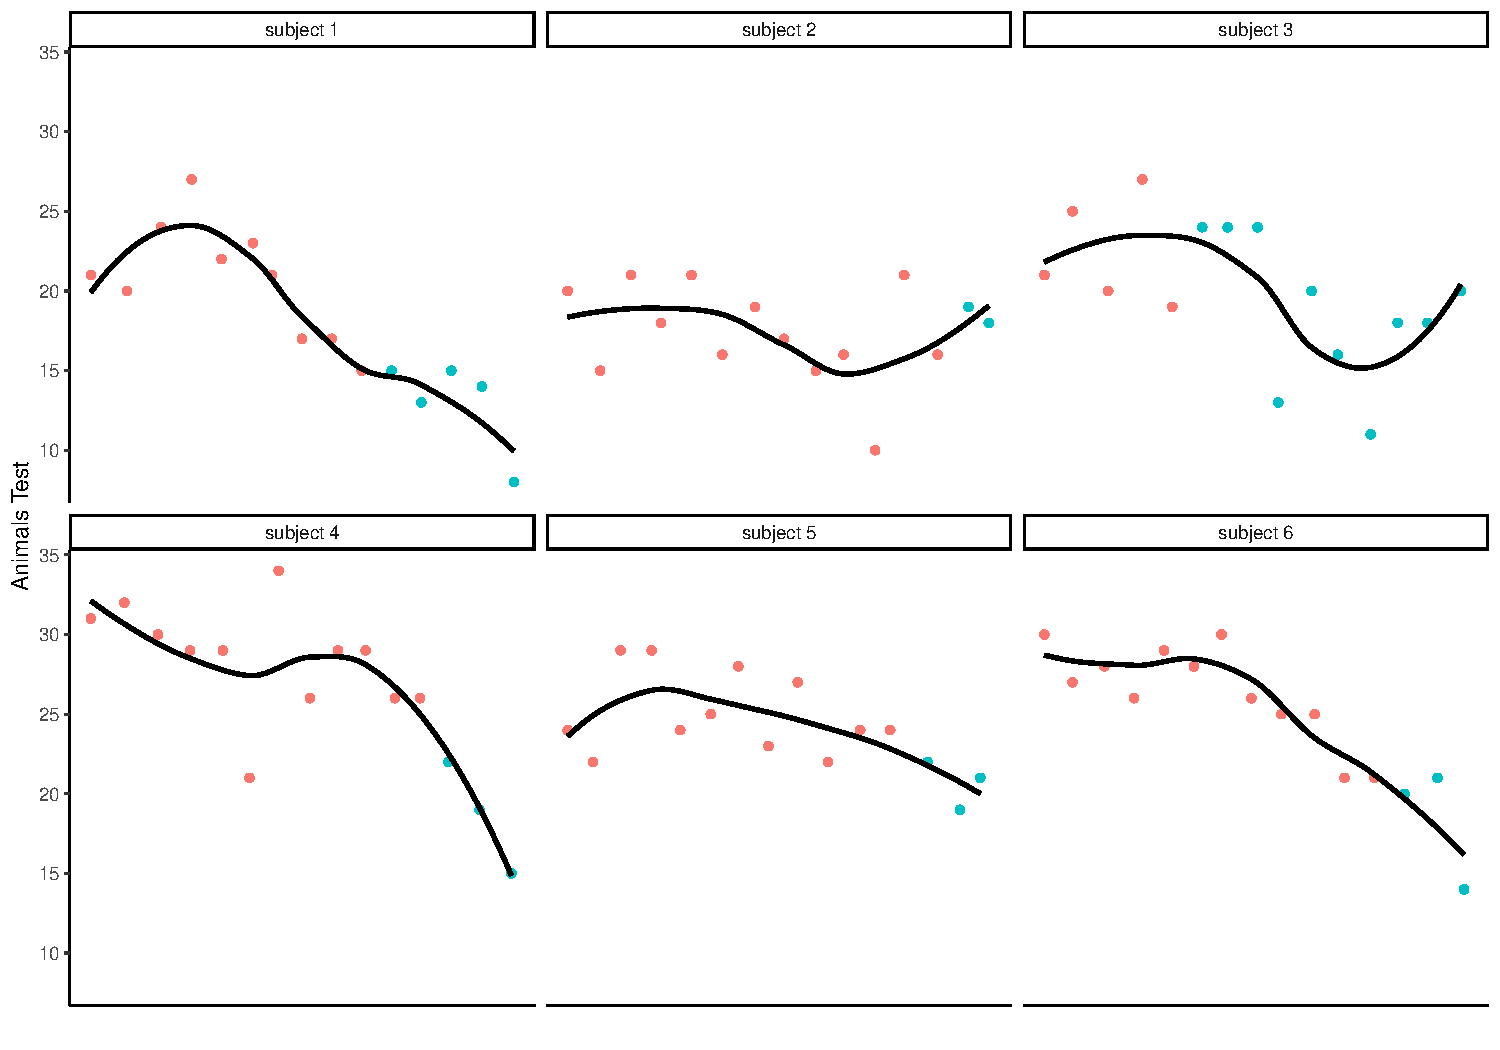
\includegraphics{Prez4_files/figure-beamer/unnamed-chunk-7-1.pdf}
\end{frame}

\begin{frame}{We Want a Model That\ldots{}}
\protect\hypertarget{we-want-a-model-that}{}
\begin{itemize}
\tightlist
\item
  Captures general trajectory.
\item
  Has the subject specific heterogeneity shown by the non-parametric
  method.
\item
  We are able to interpret and make inference on effects of interest.
\end{itemize}
\end{frame}

\begin{frame}{Welcome to the State Space Model}
\protect\hypertarget{welcome-to-the-state-space-model}{}
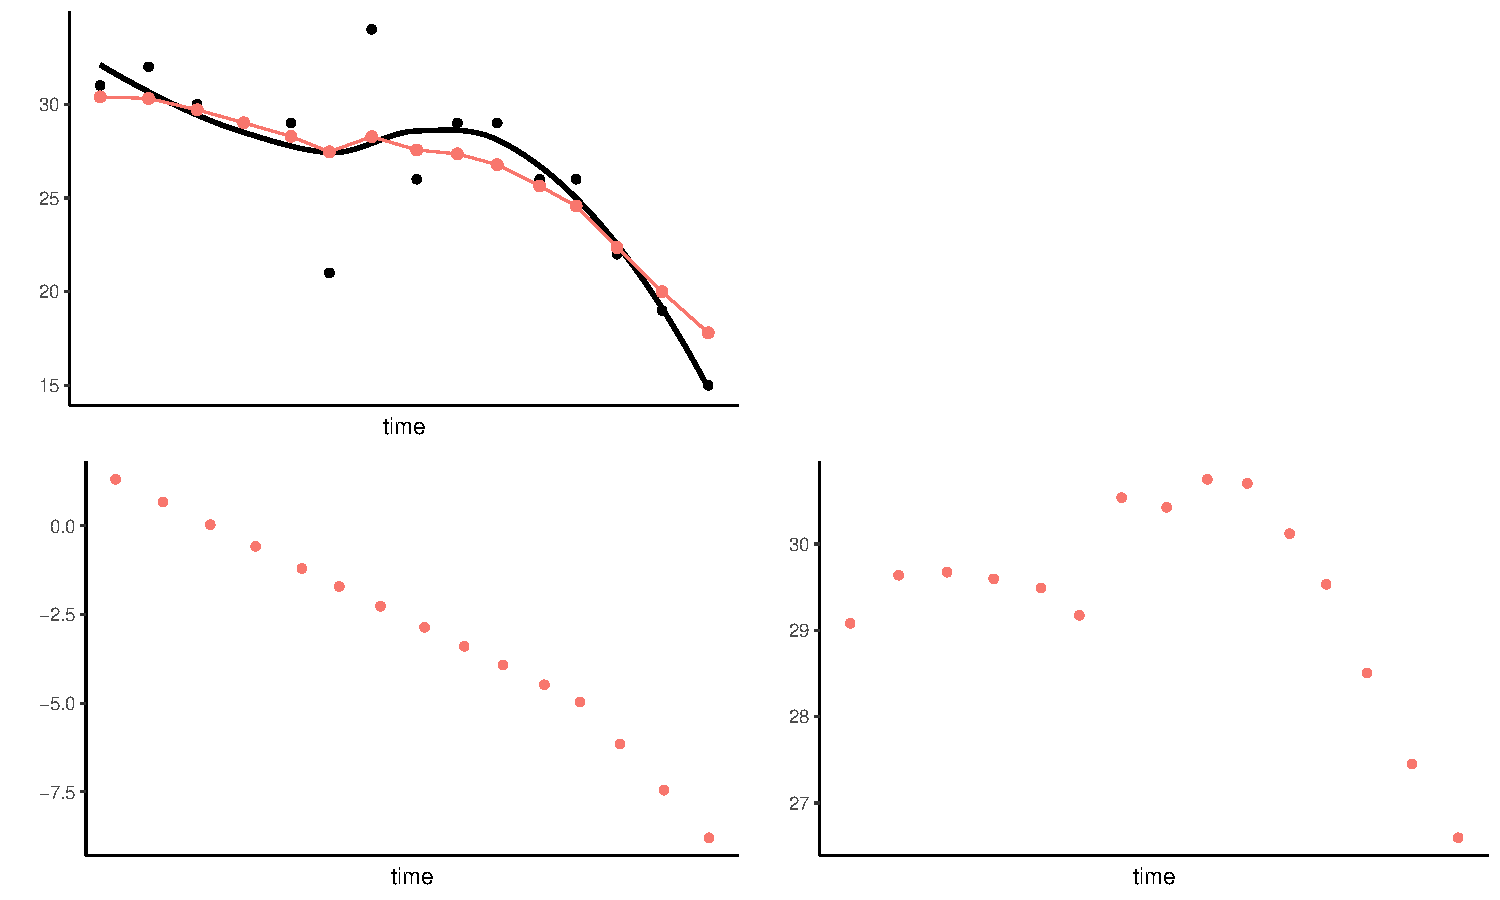
\includegraphics{Prez4_files/figure-beamer/unnamed-chunk-9-1.pdf}
\end{frame}

\begin{frame}{State Space Model Introduction}
\protect\hypertarget{state-space-model-introduction}{}
\begin{itemize}
\tightlist
\item
  State Space Models have been primarily used for time series data with
  a large number of time points and only a small number of chains
  observed.
\item
  We are working to apply these models to a small number of time points
  and a large number of subjects.

  \begin{itemize}
  \tightlist
  \item
    Small \(t\) and large \(n\) are typically what we see in
    observational data.
  \end{itemize}
\item
  We wish to show that the State Space Model can be more accommodating
  than the commonly used linear mixed effect models (LMEM)(Laird and
  Ware, 1983; Diggle, Liang and Zeger, 1994).
\end{itemize}
\end{frame}

\begin{frame}{State Space Model}
\protect\hypertarget{state-space-model}{}
A general linear state space model can be denoted as:

\begin{align*}
y_t = F_t\mu_t + v_t\\
\mu_t = G_t\mu_{t-1} + w_t
\end{align*}

where at time \(t\),

\begin{itemize}
\tightlist
\item
  \(y_t\) is the an \(n \times 1\) observation vector.
\item
  \(\mu_t\) is the \(q \times 1\) latent state vector, where \(q\) is
  the number of latent states.
\item
  \(F_t\) is the \(n \times q\) observation matrix.
\item
  \(G_t\) is the \(q \times q\) state transition matrix.
\end{itemize}

We assume \(v_t\) and \(w_t\) are independent identically distributed
with distributions \(v_t \sim N(0, V)\) and \(w_t \sim N(0,W)\)
respectively (Harvey, 1990; Durbin and Koopman, 2012) .
\end{frame}

\begin{frame}{State Space Model Illustration}
\protect\hypertarget{state-space-model-illustration}{}
General Model:

\begin{align*}
y_t = F_t\mu_t + v_t\\
\mu_t = G_t\mu_{t-1} + w_t
\end{align*}

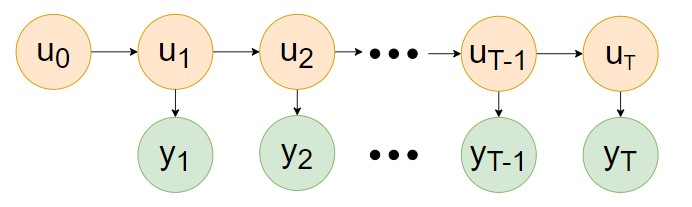
\includegraphics{images/hmm.jpg}
\end{frame}

\begin{frame}{Proposed Model}
\protect\hypertarget{proposed-model}{}
We wish to model the data according to a specific SSM, the Local Linear
Trend Model (LLT),

\begin{align*}
y_{it} &= \alpha_{it} + x_{it}^T\beta_t
+ \varepsilon_t\\
\mu_{it} =
\begin{bmatrix}
\alpha_{it}\\
\beta_{t}
\end{bmatrix} &= 
\begin{bmatrix}
\alpha_{i(t-1)}\\
\beta_{(t-1)}
\end{bmatrix} + 
\begin{bmatrix}
\eta_{it} \\
0_{p \times 1}
\end{bmatrix}
\end{align*}

Where \(\alpha_0 \sim N(a_0, P_0)\), \(\beta_0 \sim N(\beta, 0)\),
\(\varepsilon_{it} \sim N(0, \sigma^2_\varepsilon)\), and
\(\eta_{it} \sim N(0, \sigma^2_\eta)\).

\begin{itemize}
\tightlist
\item
  \(y_t\) is an \(n \times 1\) observation vector where \(n\) indicates
  the number of subjects.
\item
  \(\alpha_t\) is an \(n \times 1\) latent state vector.

  \begin{itemize}
  \tightlist
  \item
    Variation in \(\alpha_t\) over time creates a dynamic moving average
    auto-correlation between observations \(y_t\).
  \end{itemize}
\item
  \(X_t\) is an \(n \times p\) matrix of time varying covariates (can be
  \(X_t = t * X\) where \(X\) are baseline covarties).
\item
  \(\beta_t\) is the linear effect of the columns in \(X_t\).
\end{itemize}
\end{frame}

\begin{frame}{What is \(\alpha_t\)}
\protect\hypertarget{what-is-alpha_t}{}
Consider the model,

\begin{align*}
y_{it} &= \alpha_{it} + x_{it}^T\beta_t
+ \varepsilon_t\\
\mu_{it} =
\begin{bmatrix}
\alpha_{it}\\
\beta_{t}
\end{bmatrix} &= 
\begin{bmatrix}
\alpha_{i(t-1)}\\
\beta_{(t-1)}
\end{bmatrix} + 
\begin{bmatrix}
\eta_{it} \\
0_{p \times 1}
\end{bmatrix}
\end{align*}

We can think of \(\alpha_t\) as the underlying cognitive state not
accounted for by covariates \(X_t\). The \(\alpha_t\) is there to
capture unobserved effects on the outcome.

Notice \(\alpha_t|\alpha_{t-1} \sim N(\alpha_{t-1}, \sigma^2_\eta)\).
This means our next underlying cognitive state will be centered at the
previous underlying cognitive state.
\end{frame}

\begin{frame}{Revisited Plot}
\protect\hypertarget{revisited-plot}{}
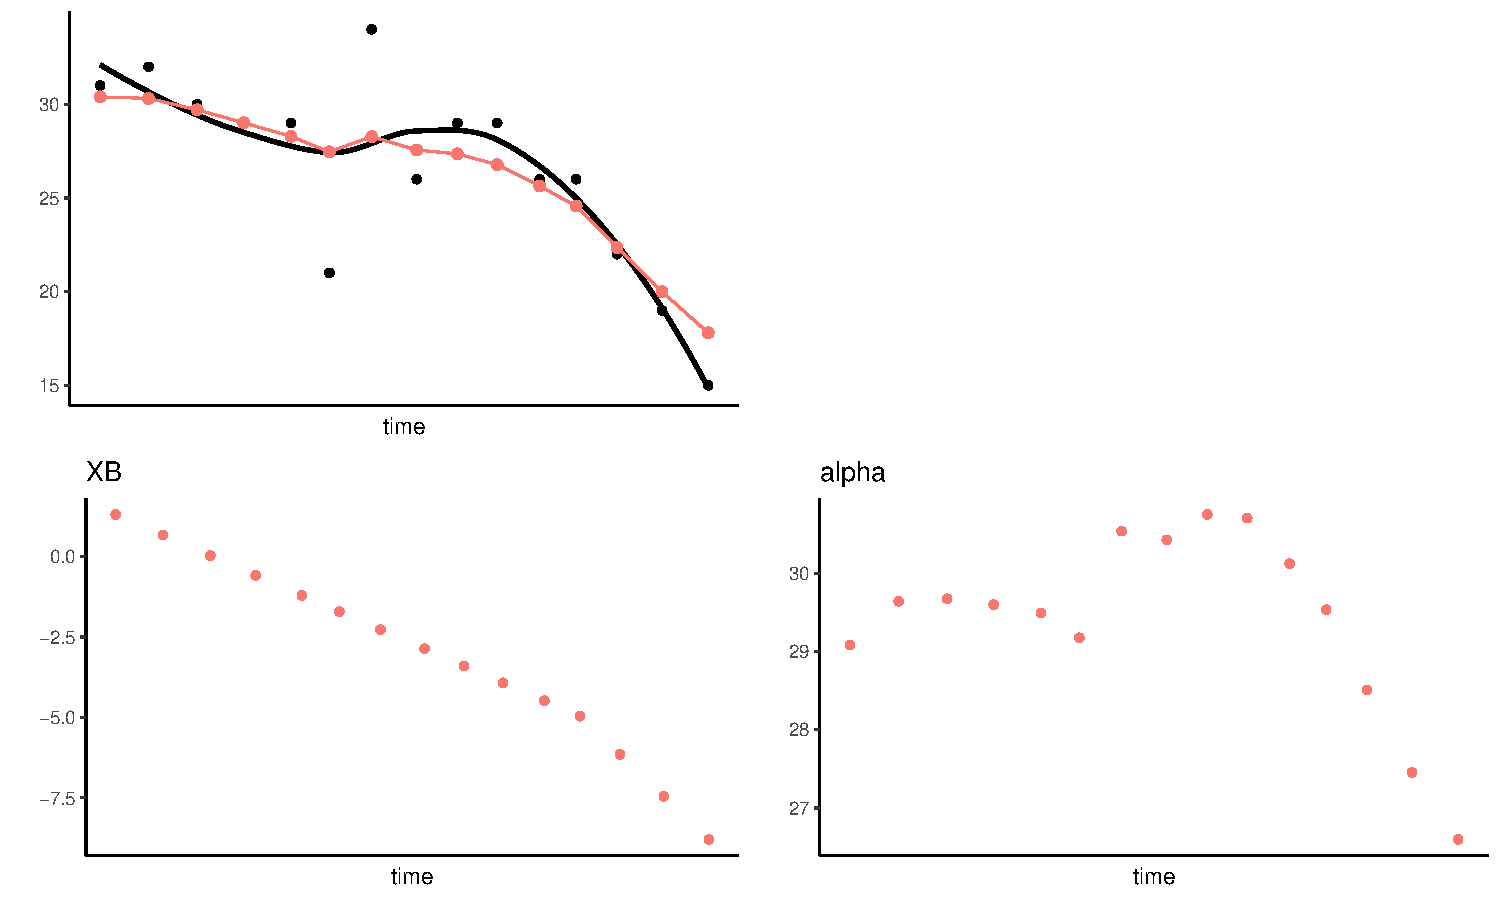
\includegraphics{Prez4_files/figure-beamer/unnamed-chunk-10-1.pdf}
\end{frame}

\begin{frame}{Single subject from an LLT}
\protect\hypertarget{single-subject-from-an-llt}{}
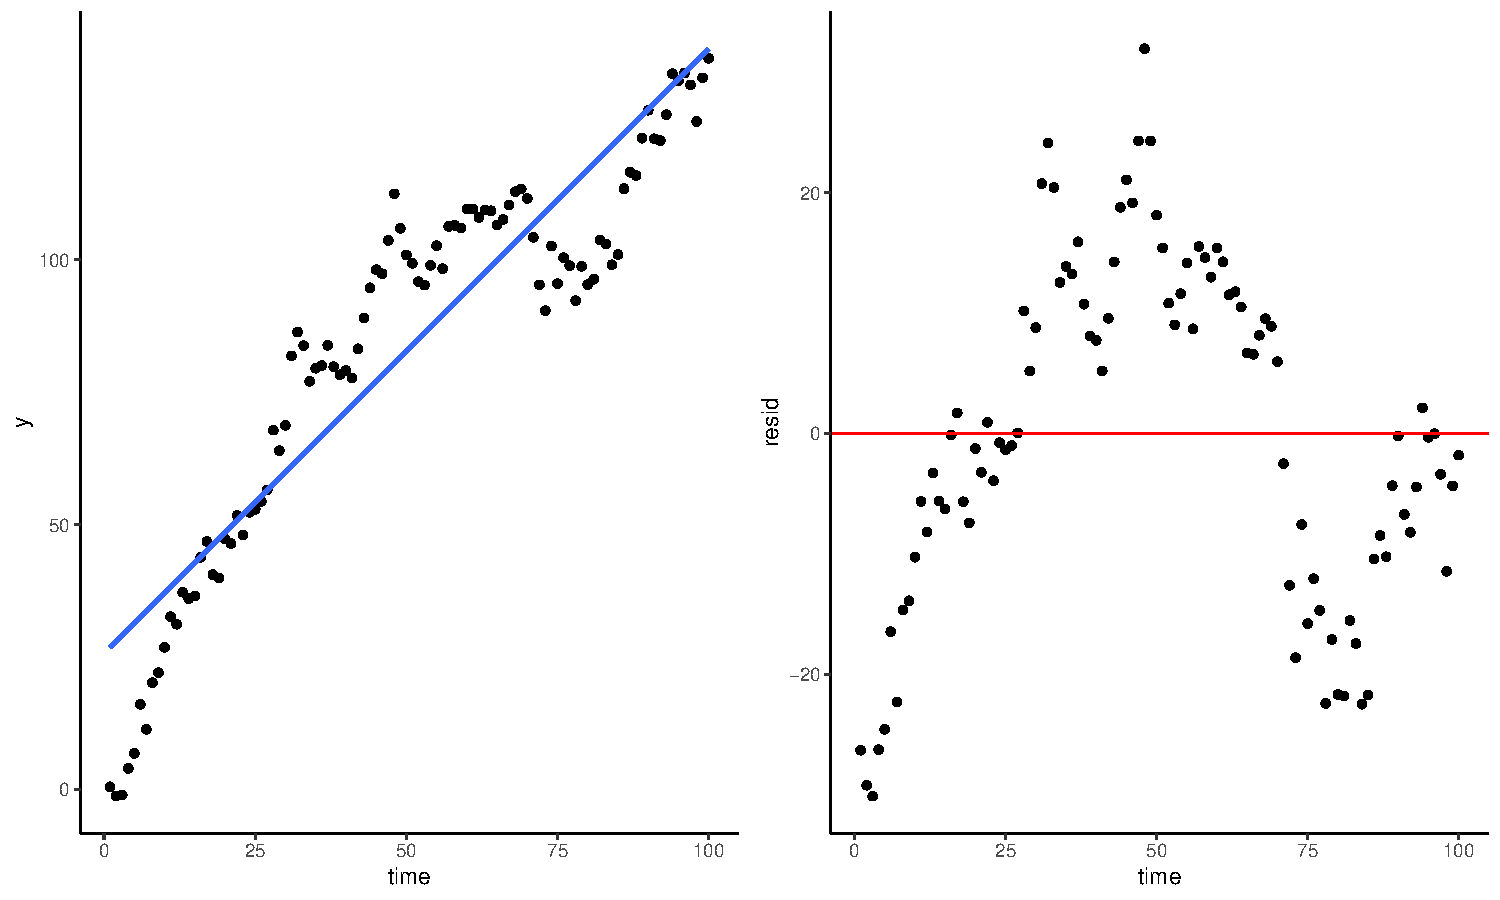
\includegraphics{Prez4_files/figure-beamer/unnamed-chunk-11-1.pdf}
\end{frame}

\begin{frame}{Auto-correlation}
\protect\hypertarget{auto-correlation}{}
The correlation between observations at any two time points is called
the auto-correlation.

Our proposed SSM model has the following auto correlation structure.

\begin{align*}
corr(y_{it}, y_{i(t+\tau)}) = \frac{t\sigma^2_\eta}{\sqrt{\sigma^2_\varepsilon + t\sigma^2_\eta}\sqrt{\sigma^2_\varepsilon + (t+\tau)\sigma^2_\eta}}
\end{align*}

This is equivalent to a dynamic moving average covariance structure. If
\(\sigma^2_\eta = 0\) then auto-correlation is 0 and our proposed model
boils down to a LMEM.

\begin{align*}
y_t &= \alpha_0 + X_t\beta
+ \varepsilon_t\\
\end{align*}
\end{frame}

\begin{frame}{Accounting for Autocorrelation in LMEM Framework}
\protect\hypertarget{accounting-for-autocorrelation-in-lmem-framework}{}
\begin{itemize}
\tightlist
\item
  Many different autocorrelation techniques have been used.
\item
  A common practice has been to model an AR(1) covariance structure on
  the errors.
\end{itemize}

\begin{equation*}
\begin{aligned}
y_t &= b_0 + X_t \beta + e_t, \ \ \ b_0\sim N(0, \sigma^2_b)\\
e_t &= \rho e_{t-1} + \eta_t, \ \ \ \eta_t \sim N(0, \sigma^2_\eta), \ \ \ -1 < \rho < 1
\end{aligned}
\end{equation*}
\end{frame}

\begin{frame}{Lots of Plots}
\protect\hypertarget{lots-of-plots}{}
\begin{itemize}
\tightlist
\item
  The next few plots show the \(E(Y_{t+\tau}|Y_t, \beta, X)\).
\item
  Illustrates the LLT allows for dynamic changes in predicted trajectory
  while the LMEM and LMEM with AR(1) are very restrictive.
\end{itemize}
\end{frame}

\begin{frame}{}
\protect\hypertarget{section}{}
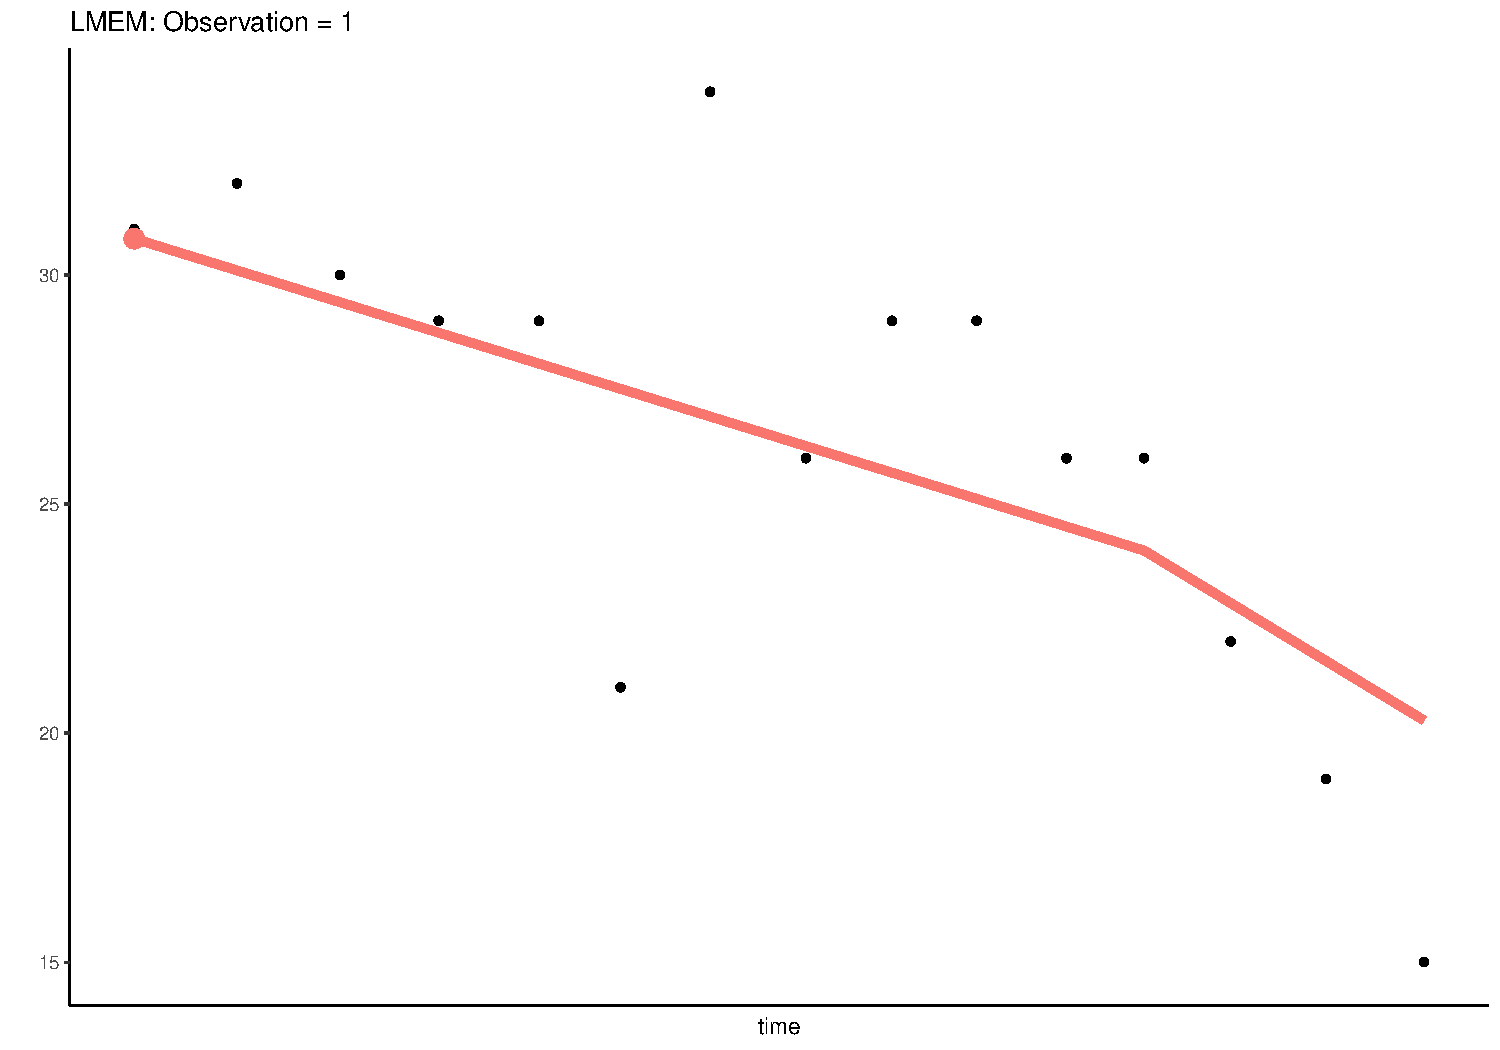
\includegraphics{Prez4_files/figure-beamer/unnamed-chunk-13-1.pdf}
\end{frame}

\begin{frame}{}
\protect\hypertarget{section-1}{}
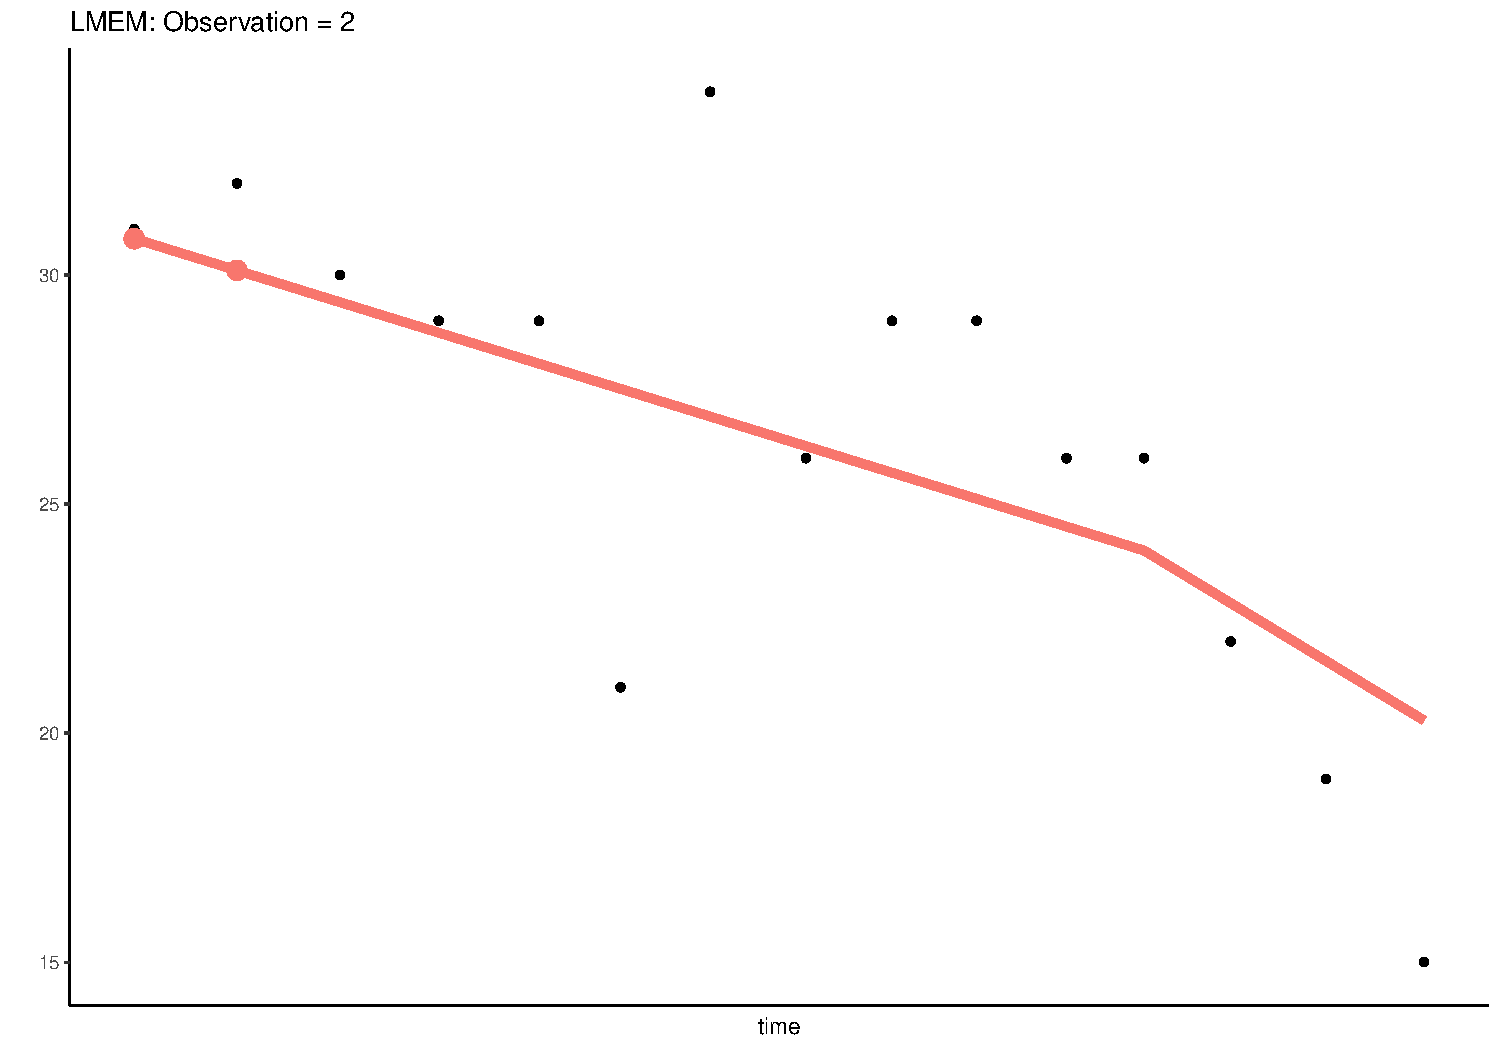
\includegraphics{Prez4_files/figure-beamer/unnamed-chunk-13-2.pdf}
\end{frame}

\begin{frame}{}
\protect\hypertarget{section-2}{}
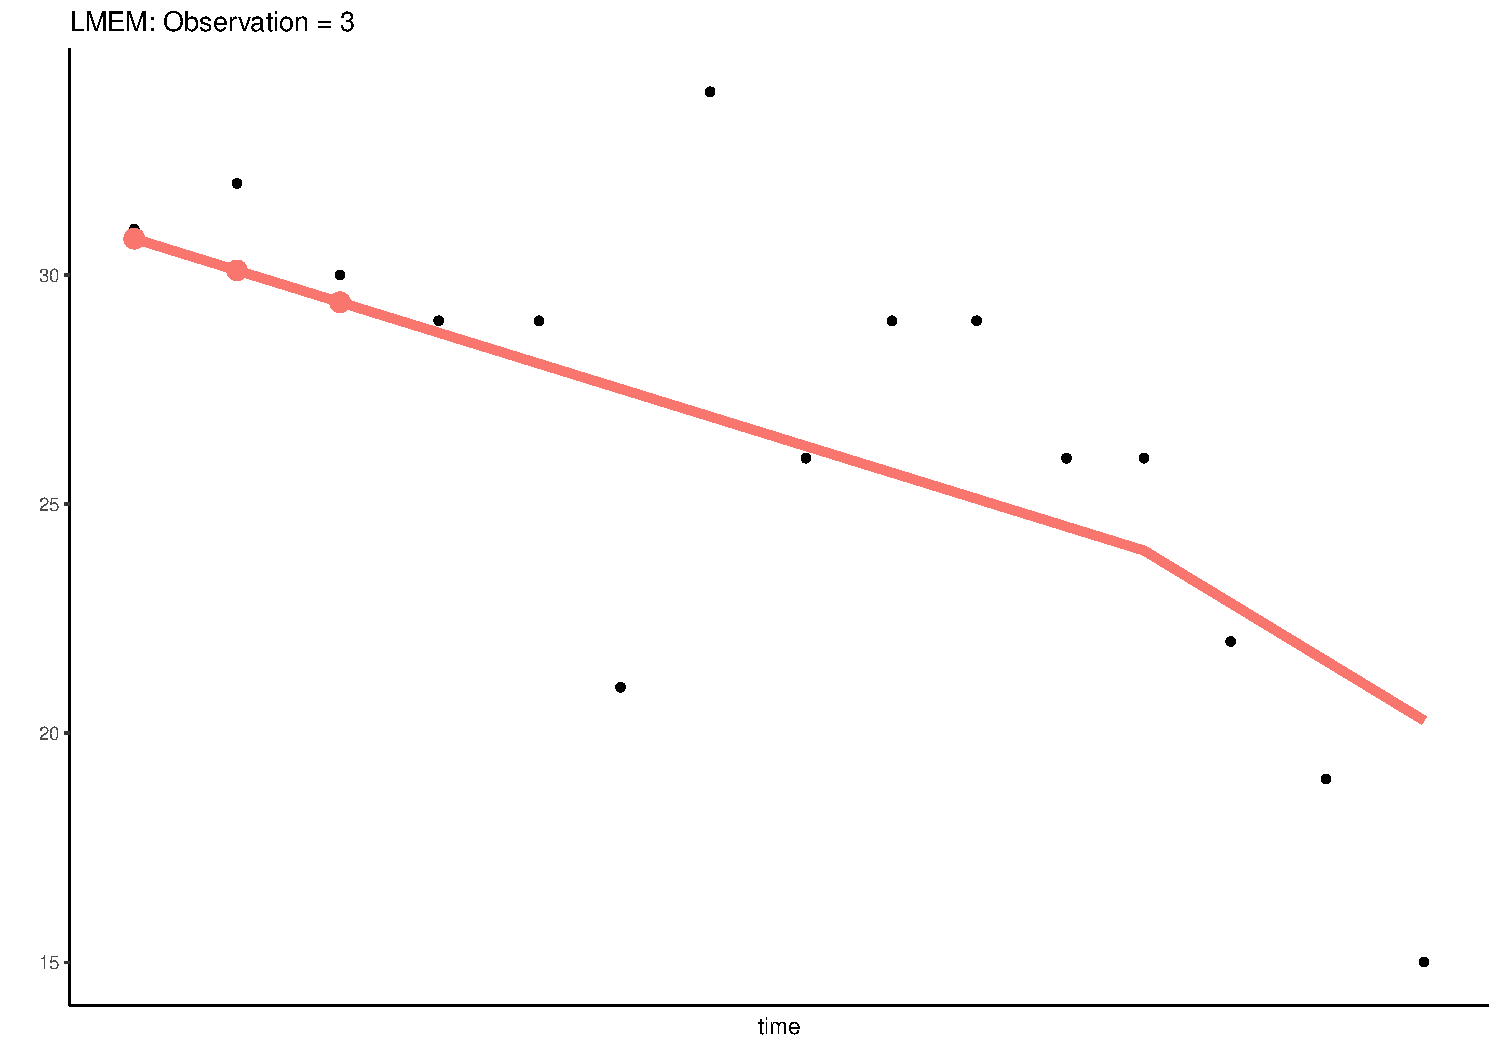
\includegraphics{Prez4_files/figure-beamer/unnamed-chunk-13-3.pdf}
\end{frame}

\begin{frame}{}
\protect\hypertarget{section-3}{}
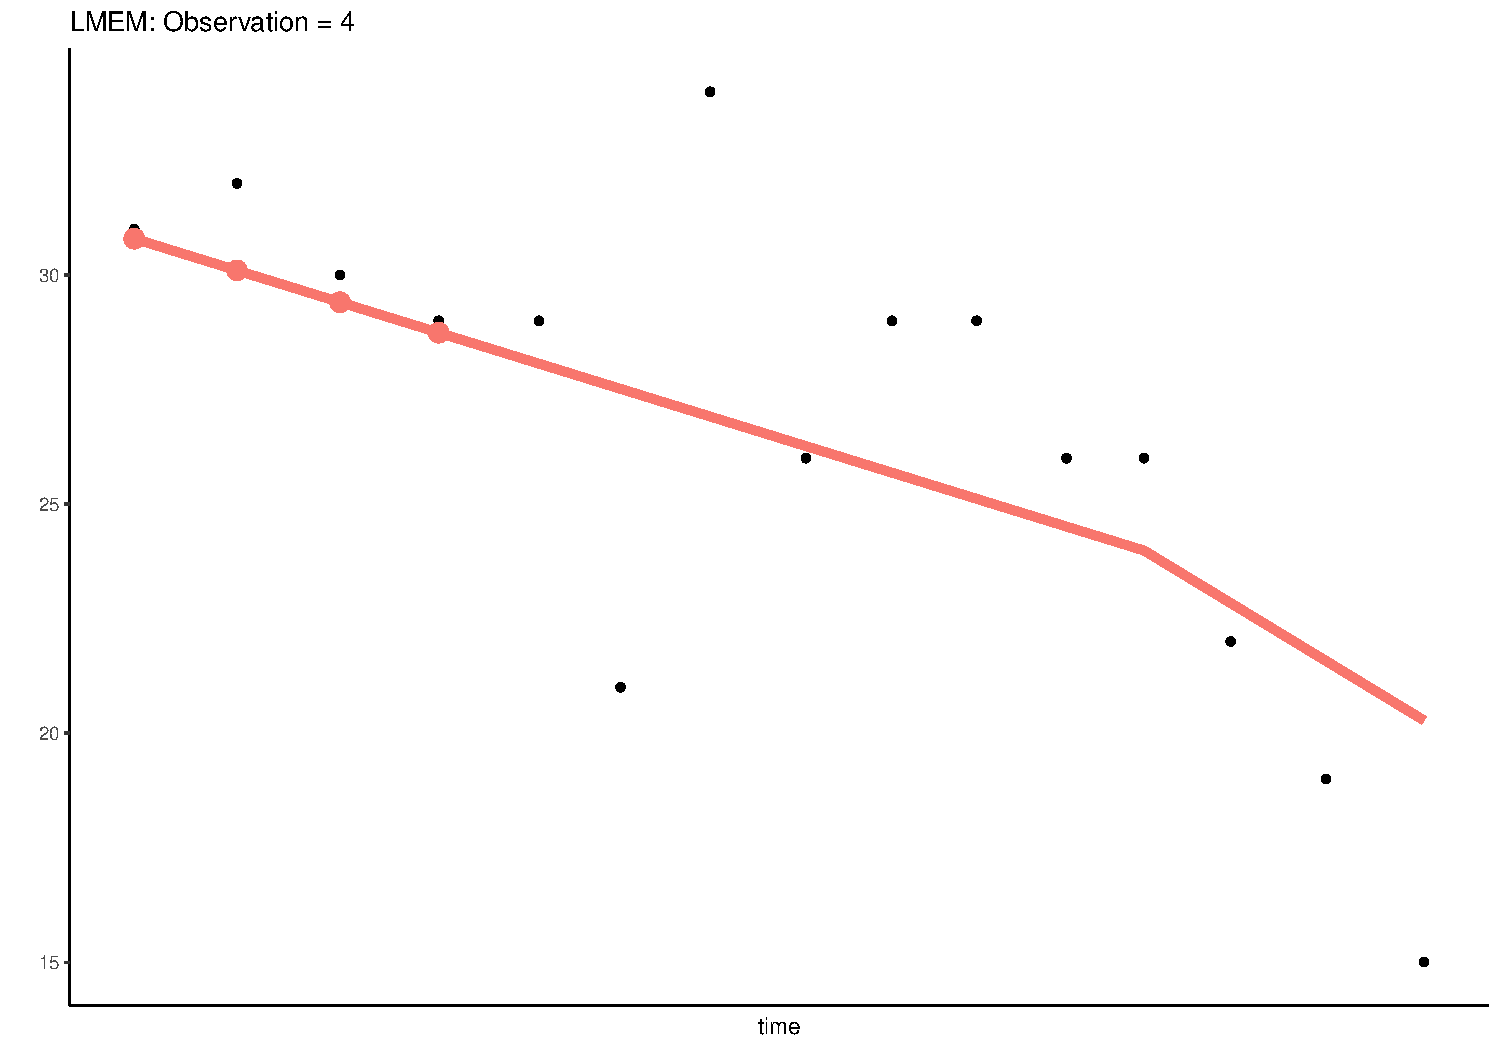
\includegraphics{Prez4_files/figure-beamer/unnamed-chunk-13-4.pdf}
\end{frame}

\begin{frame}{}
\protect\hypertarget{section-4}{}
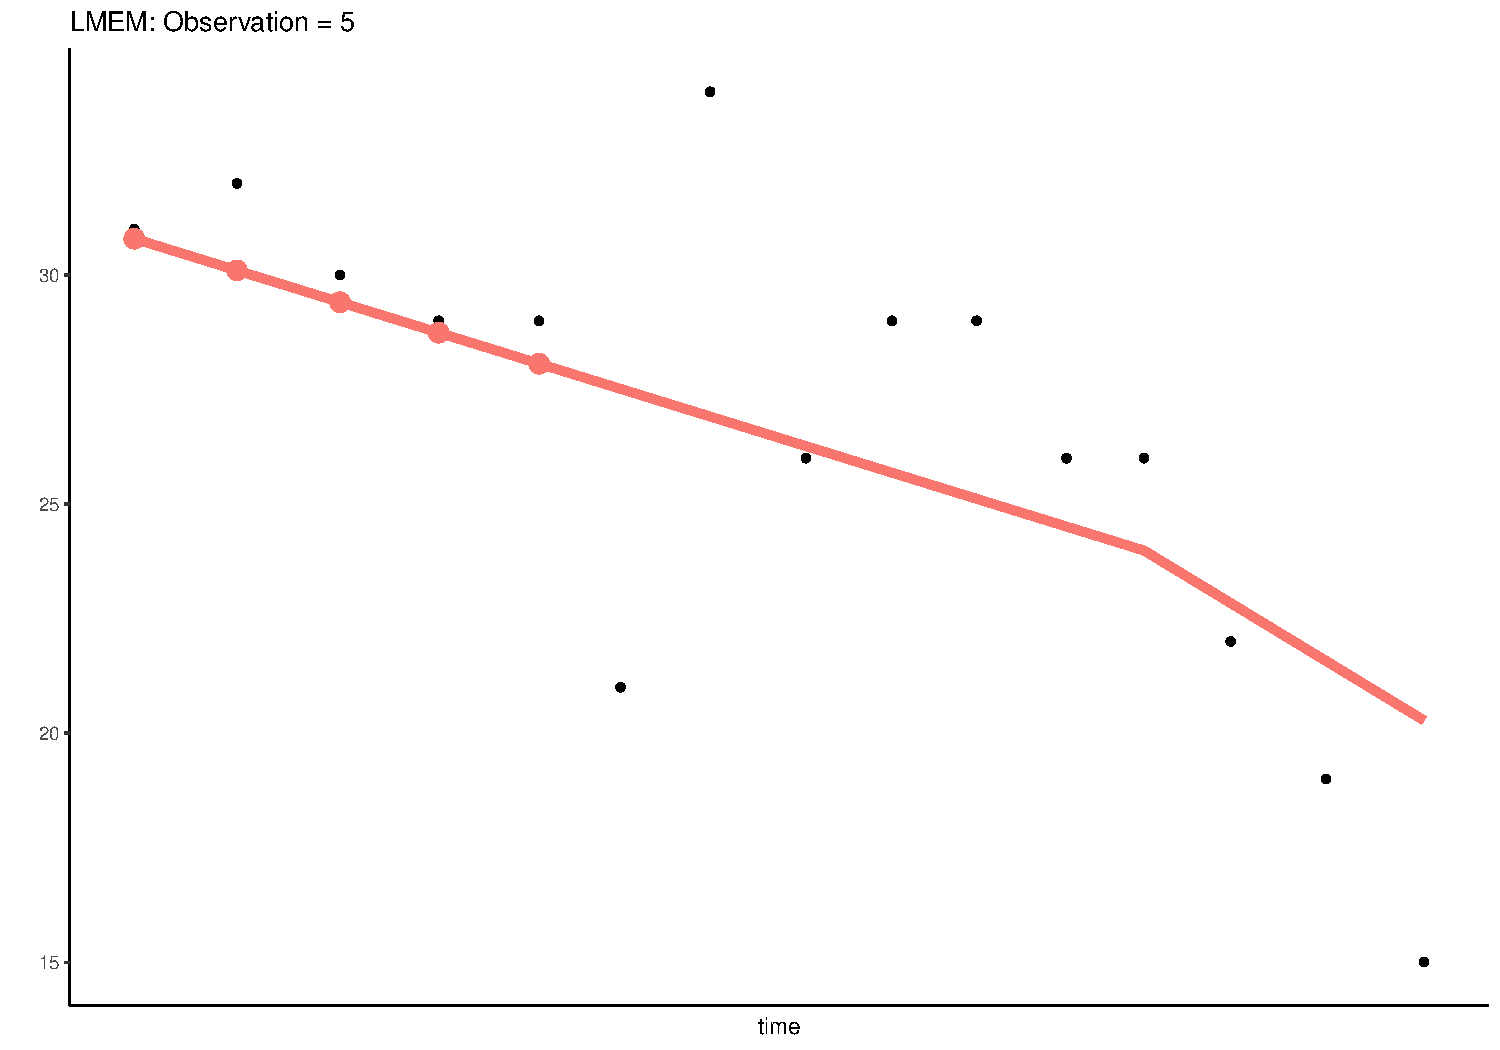
\includegraphics{Prez4_files/figure-beamer/unnamed-chunk-13-5.pdf}
\end{frame}

\begin{frame}{}
\protect\hypertarget{section-5}{}
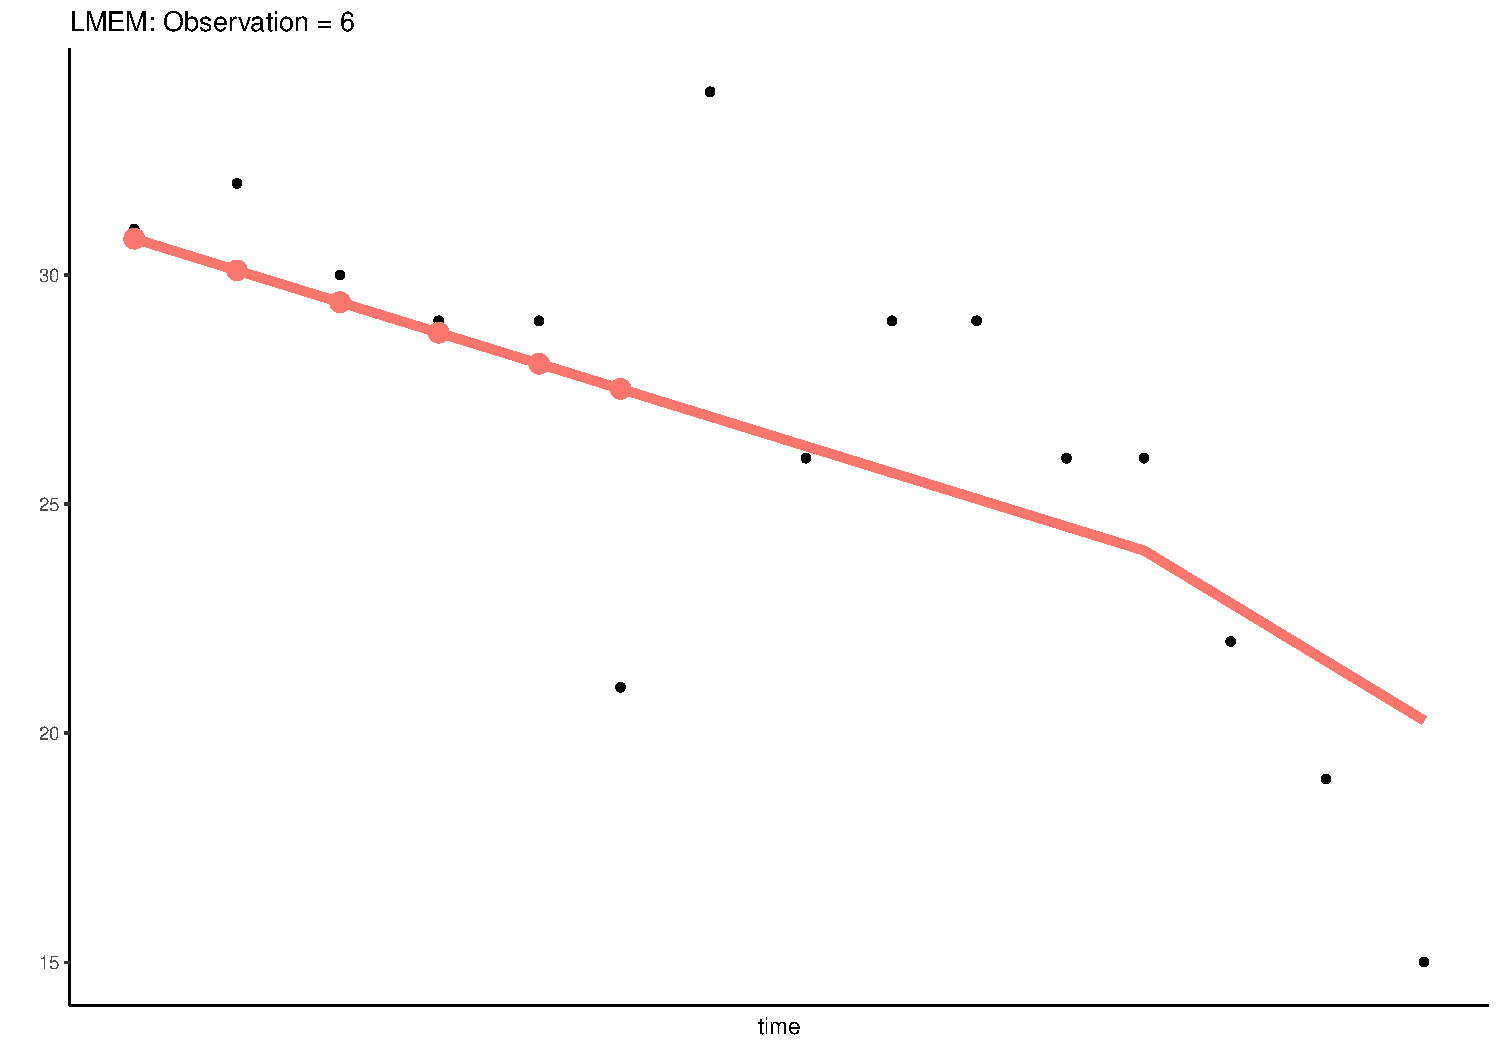
\includegraphics{Prez4_files/figure-beamer/unnamed-chunk-13-6.pdf}
\end{frame}

\begin{frame}{}
\protect\hypertarget{section-6}{}
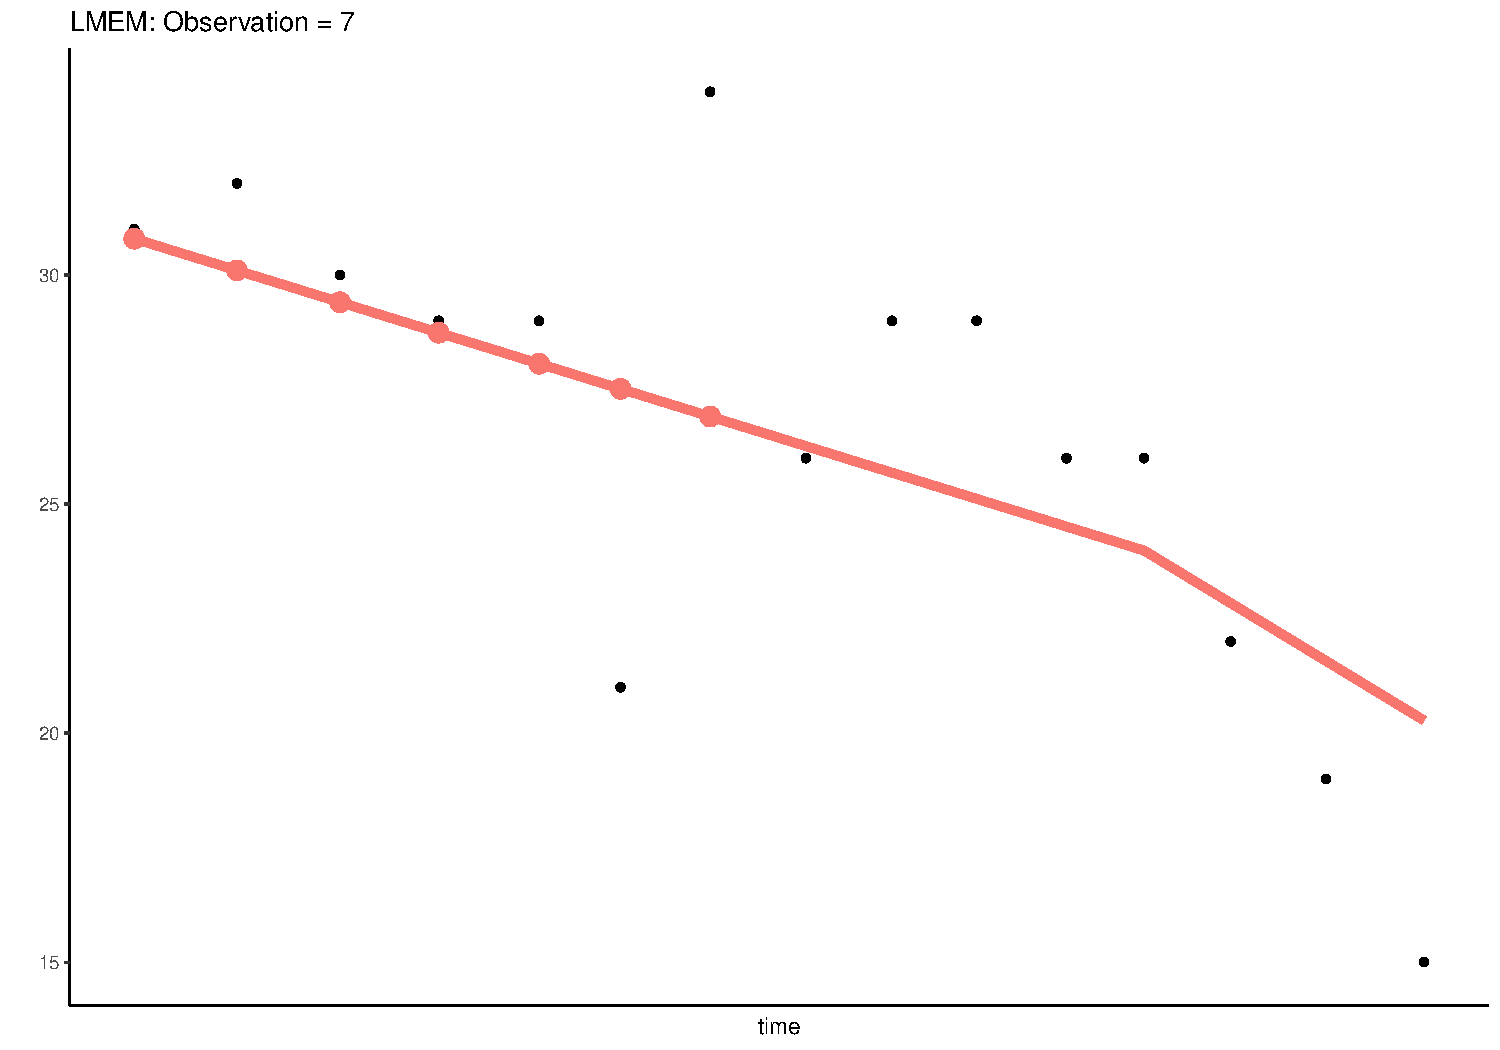
\includegraphics{Prez4_files/figure-beamer/unnamed-chunk-13-7.pdf}
\end{frame}

\begin{frame}{}
\protect\hypertarget{section-7}{}
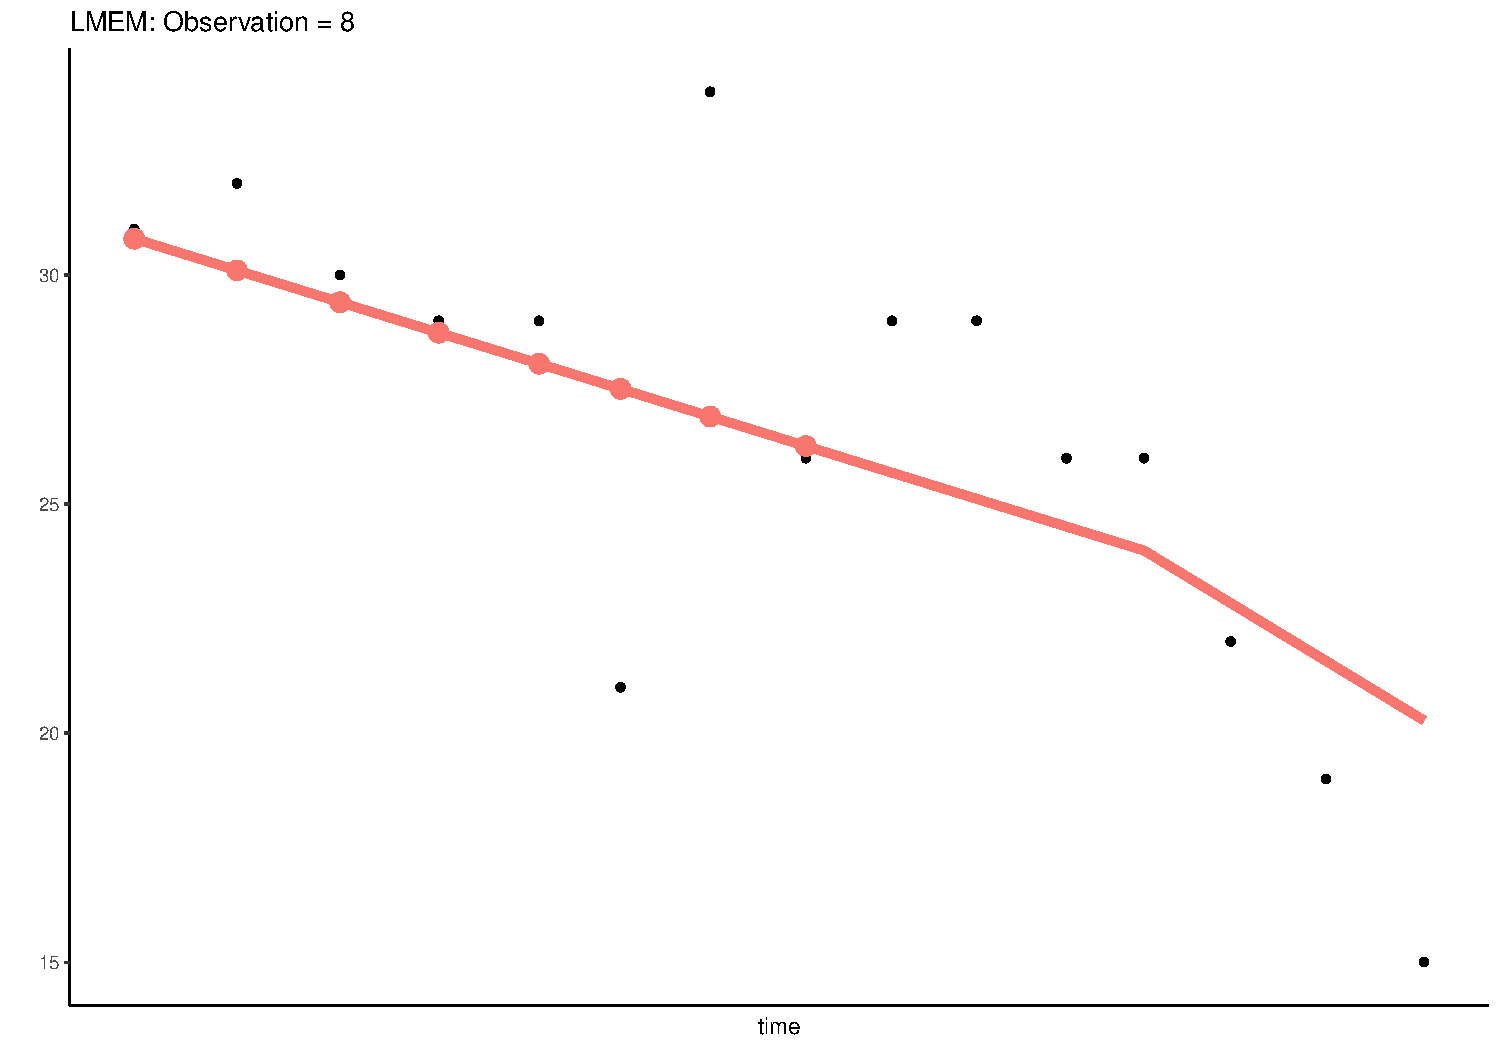
\includegraphics{Prez4_files/figure-beamer/unnamed-chunk-13-8.pdf}
\end{frame}

\begin{frame}{}
\protect\hypertarget{section-8}{}
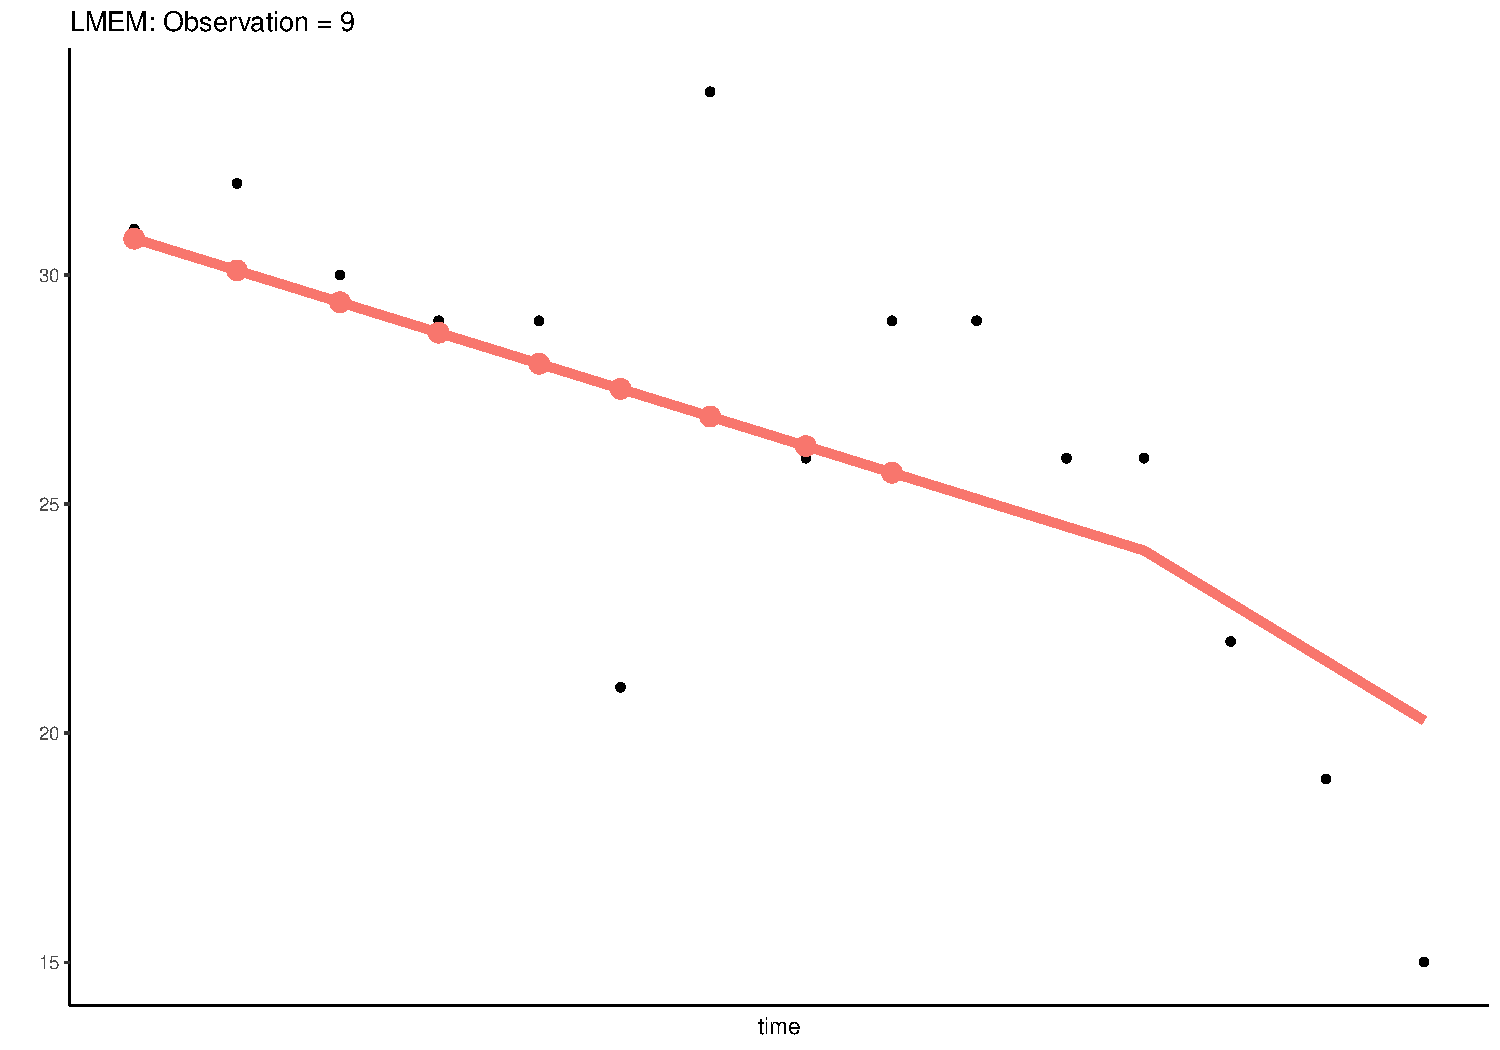
\includegraphics{Prez4_files/figure-beamer/unnamed-chunk-13-9.pdf}
\end{frame}

\begin{frame}{}
\protect\hypertarget{section-9}{}
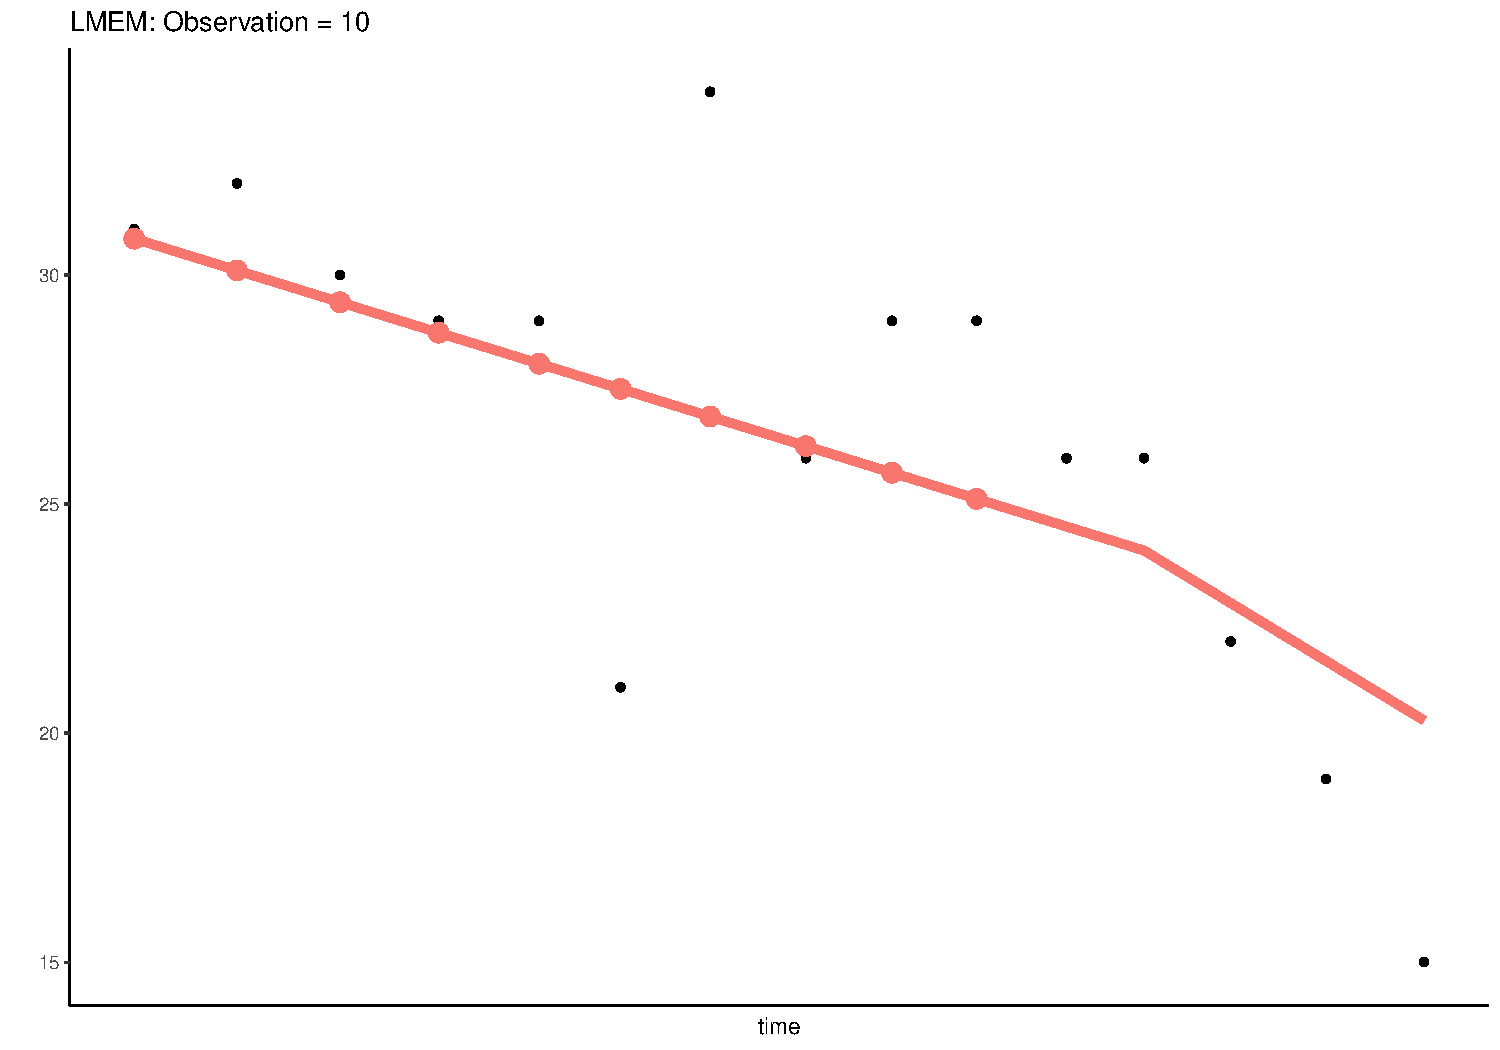
\includegraphics{Prez4_files/figure-beamer/unnamed-chunk-13-10.pdf}
\end{frame}

\begin{frame}{}
\protect\hypertarget{section-10}{}
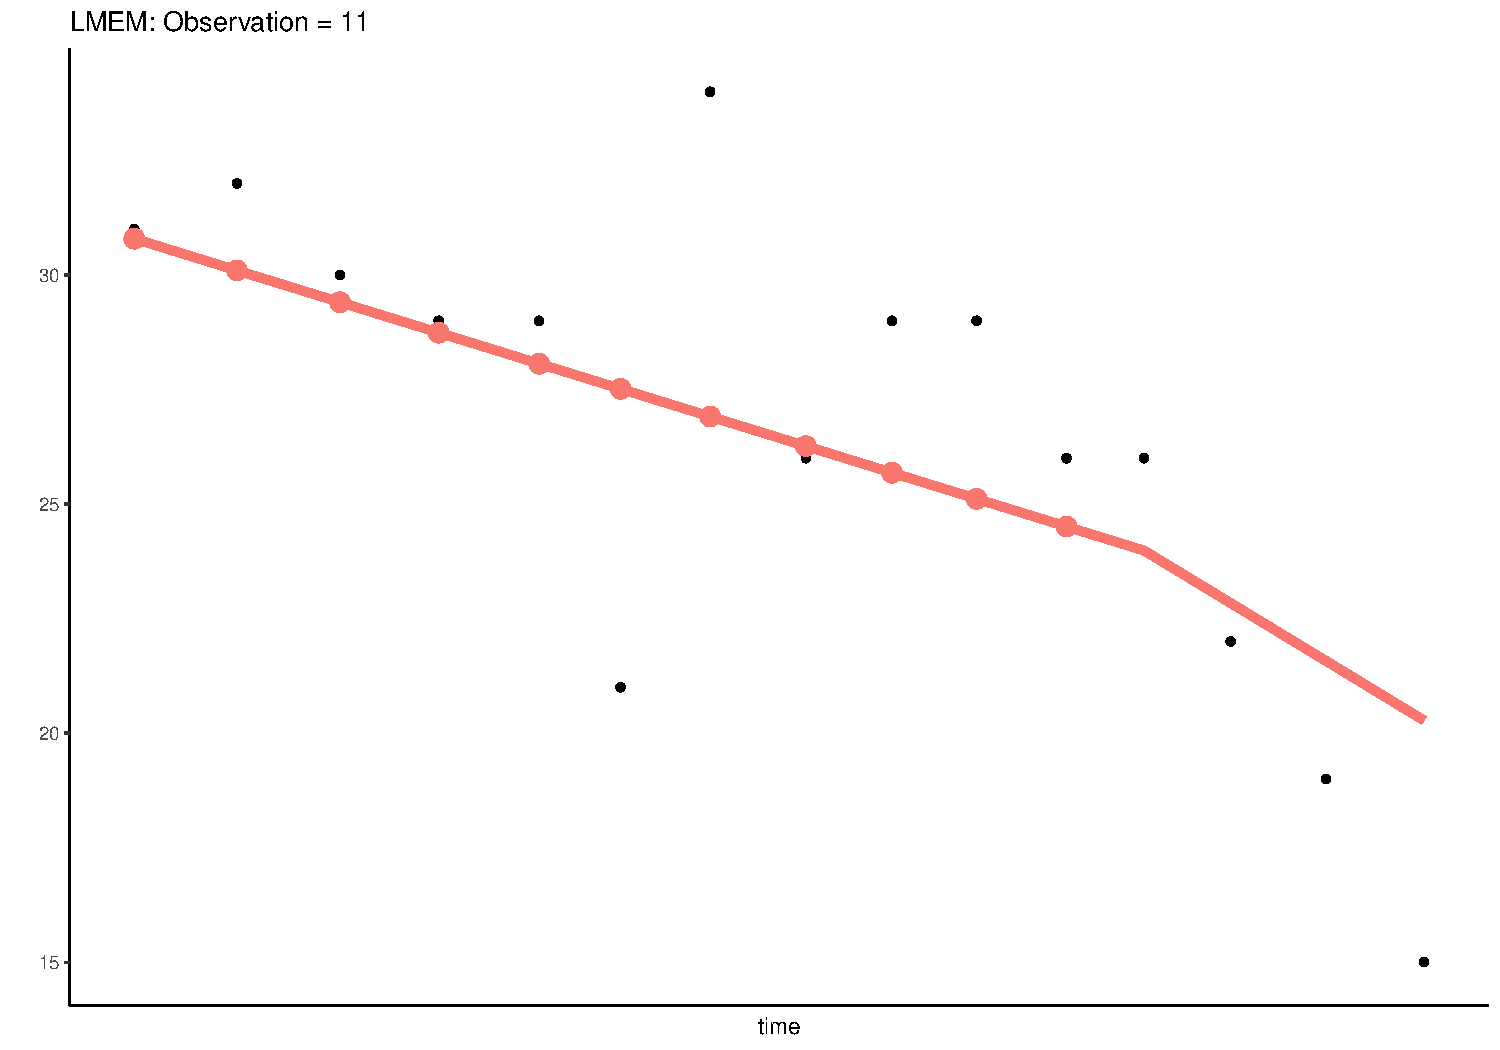
\includegraphics{Prez4_files/figure-beamer/unnamed-chunk-13-11.pdf}
\end{frame}

\begin{frame}{}
\protect\hypertarget{section-11}{}
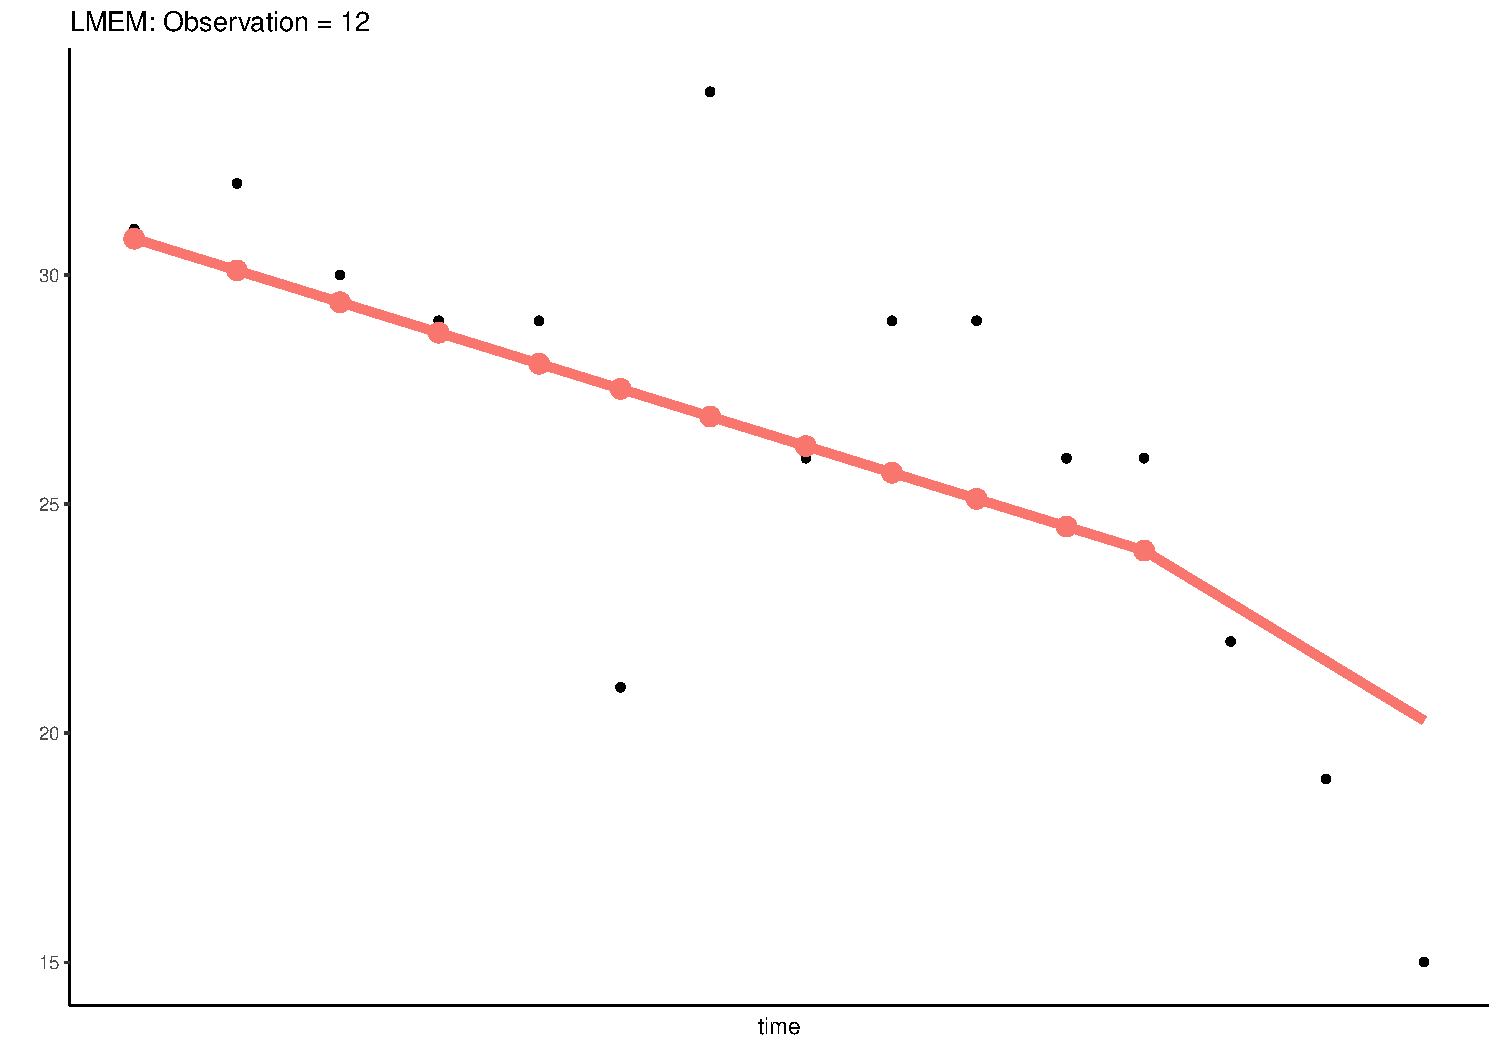
\includegraphics{Prez4_files/figure-beamer/unnamed-chunk-13-12.pdf}
\end{frame}

\begin{frame}{}
\protect\hypertarget{section-12}{}
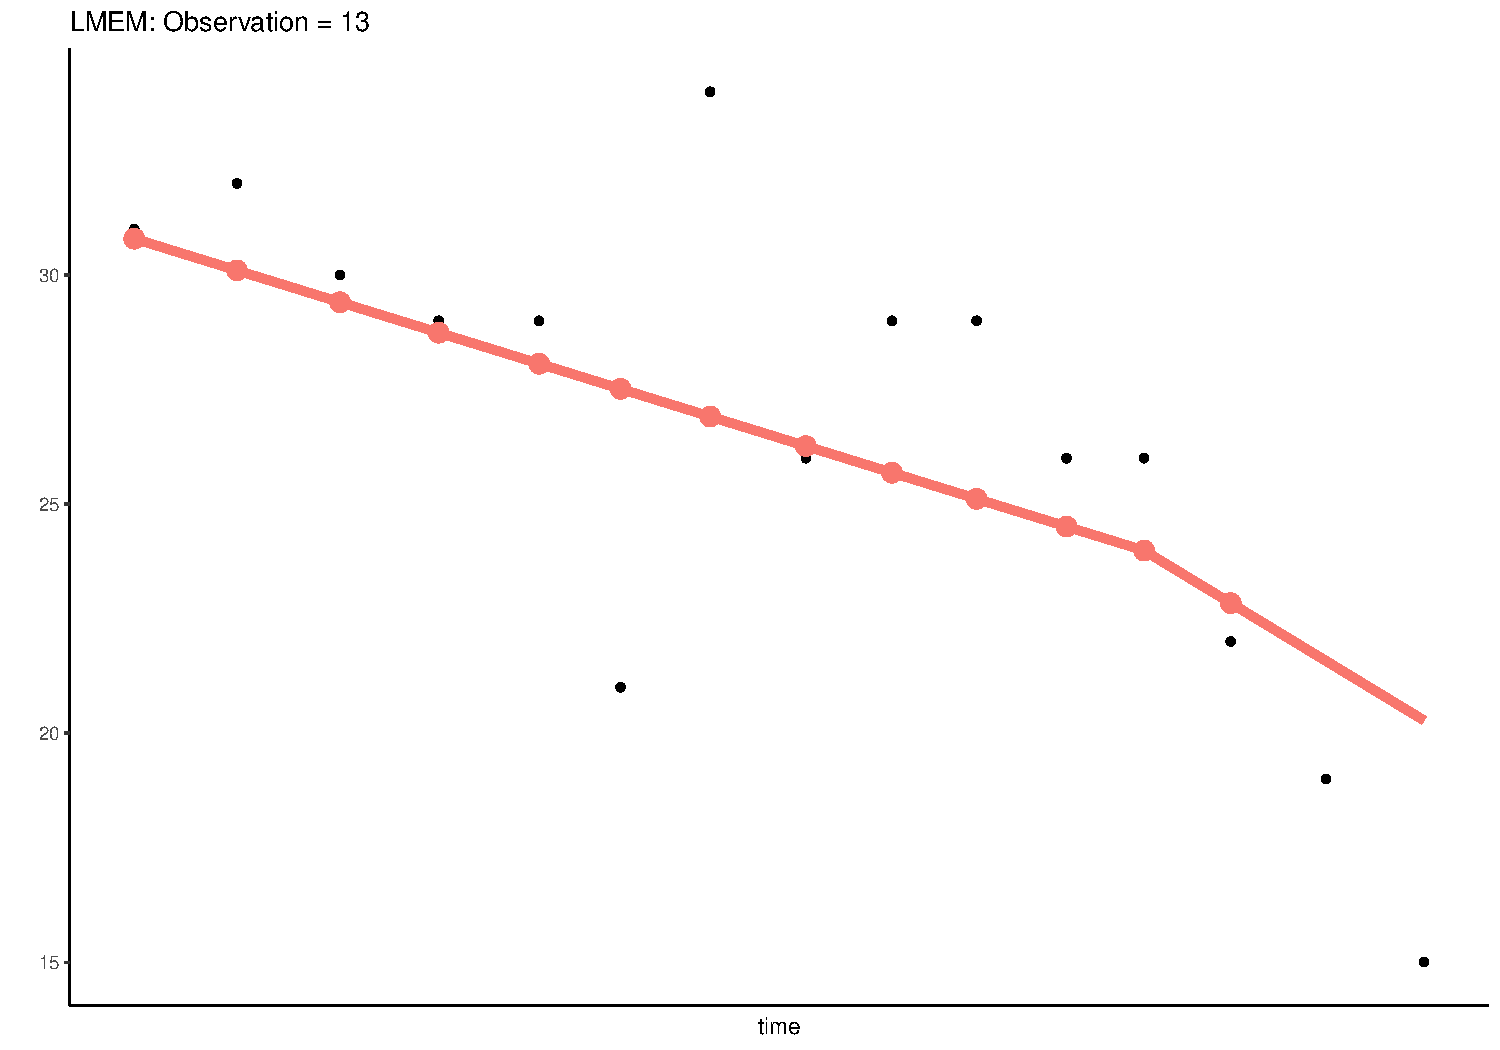
\includegraphics{Prez4_files/figure-beamer/unnamed-chunk-13-13.pdf}
\end{frame}

\begin{frame}{}
\protect\hypertarget{section-13}{}
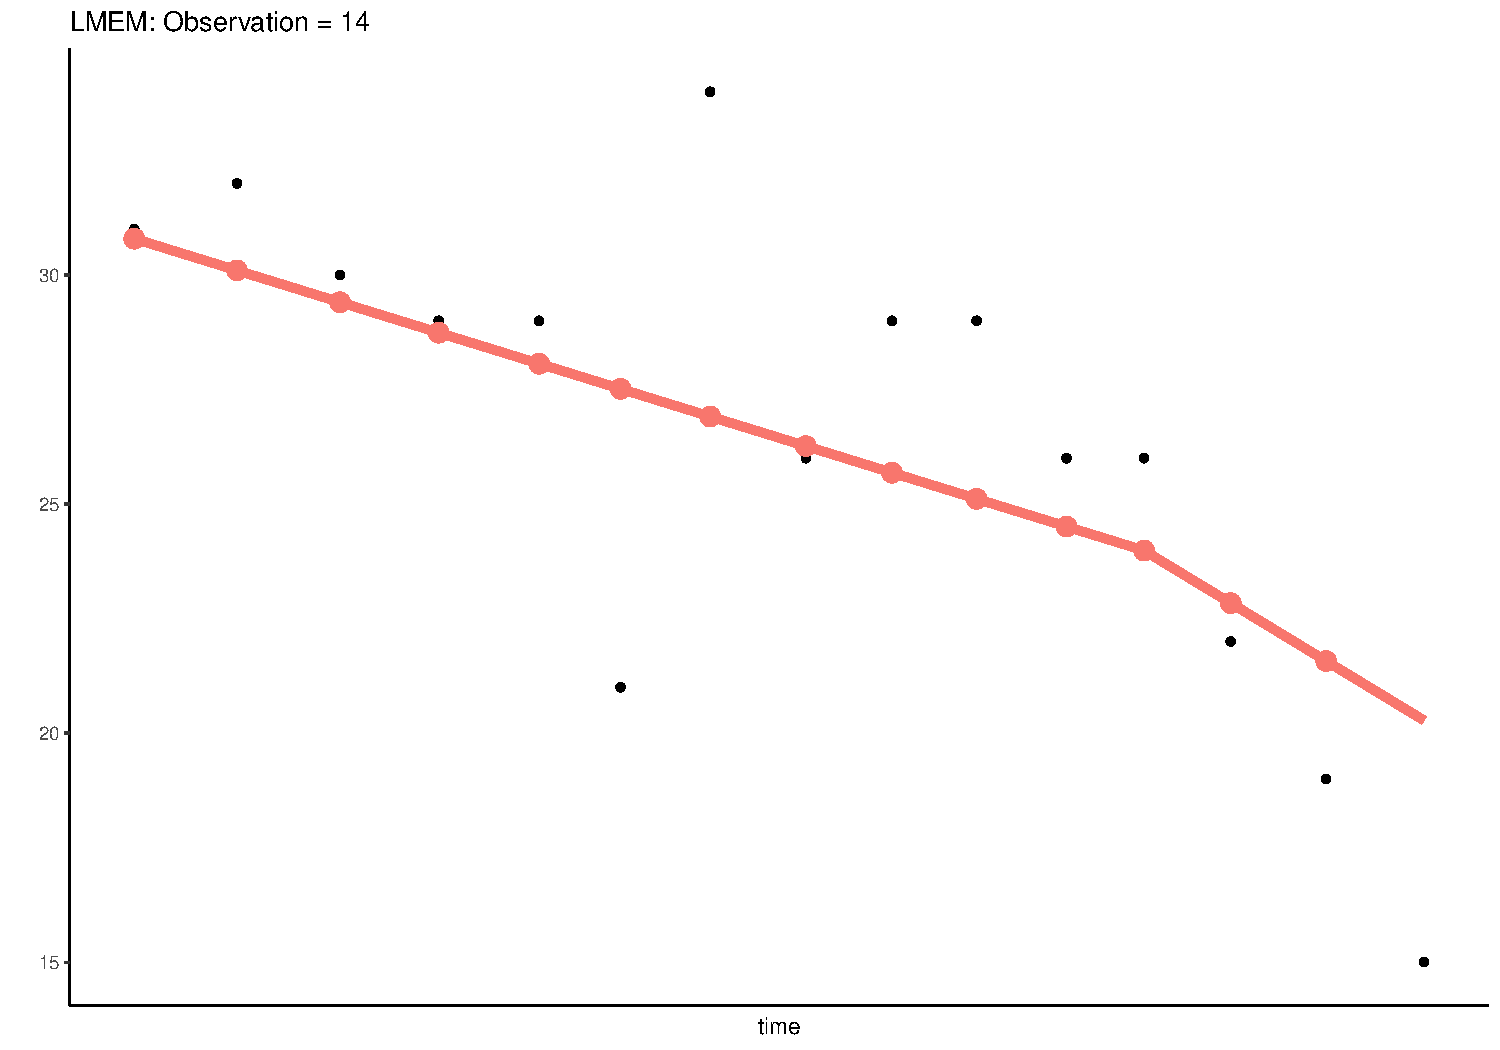
\includegraphics{Prez4_files/figure-beamer/unnamed-chunk-13-14.pdf}
\end{frame}

\begin{frame}{}
\protect\hypertarget{section-14}{}
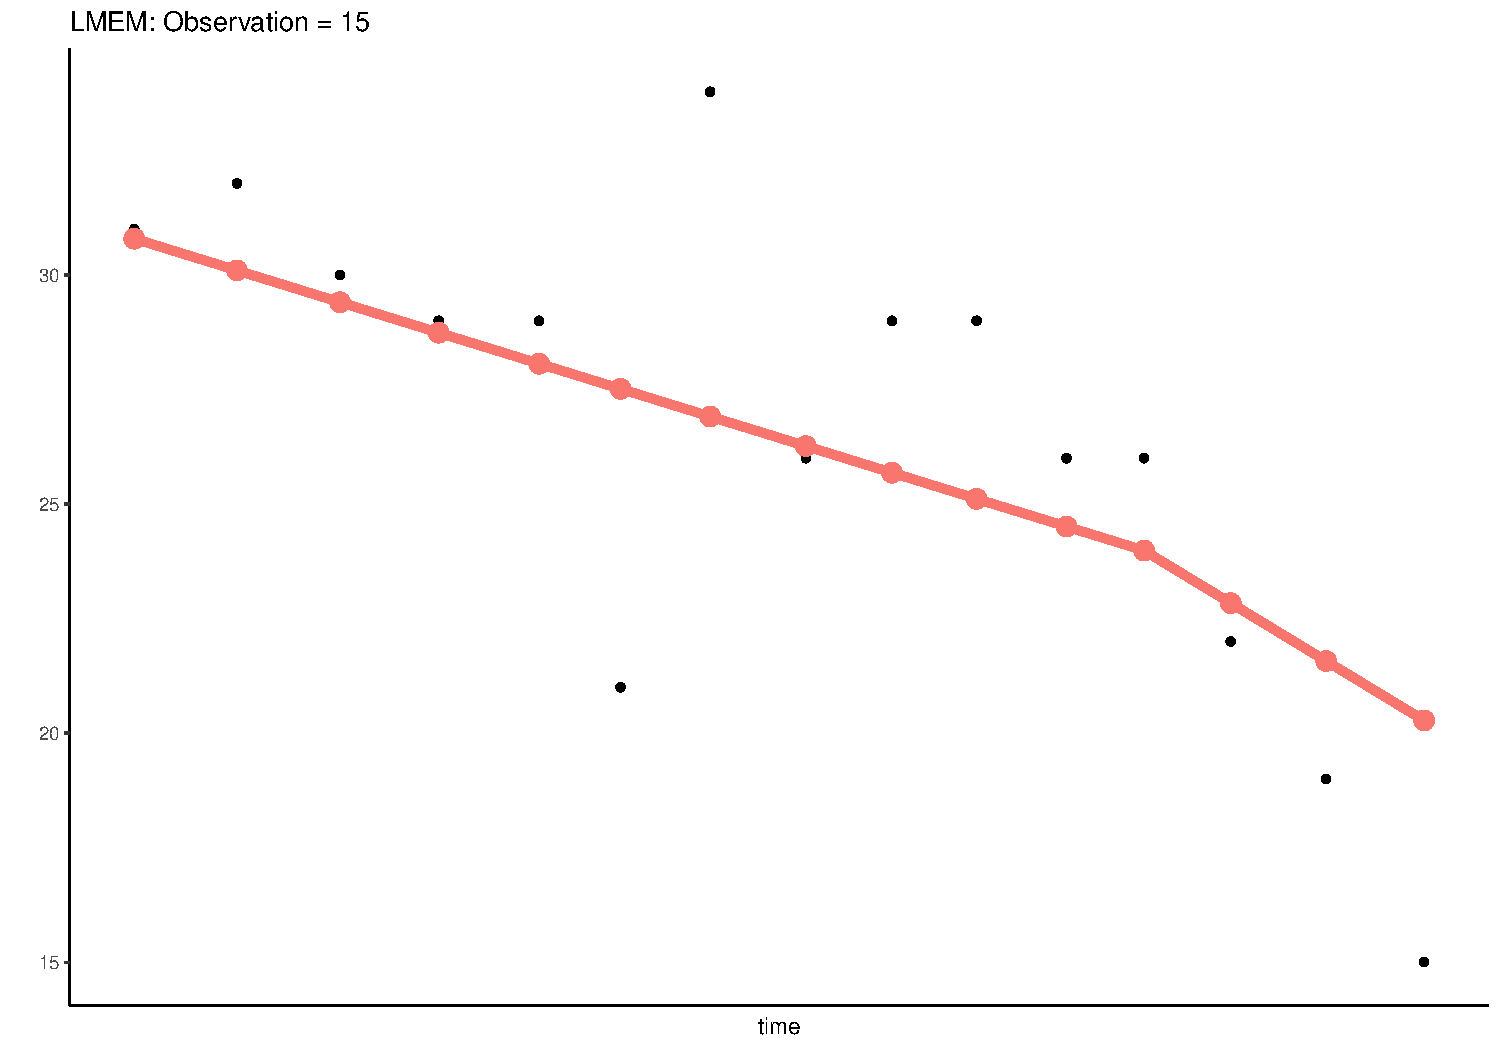
\includegraphics{Prez4_files/figure-beamer/unnamed-chunk-13-15.pdf}
\end{frame}

\begin{frame}{}
\protect\hypertarget{section-15}{}
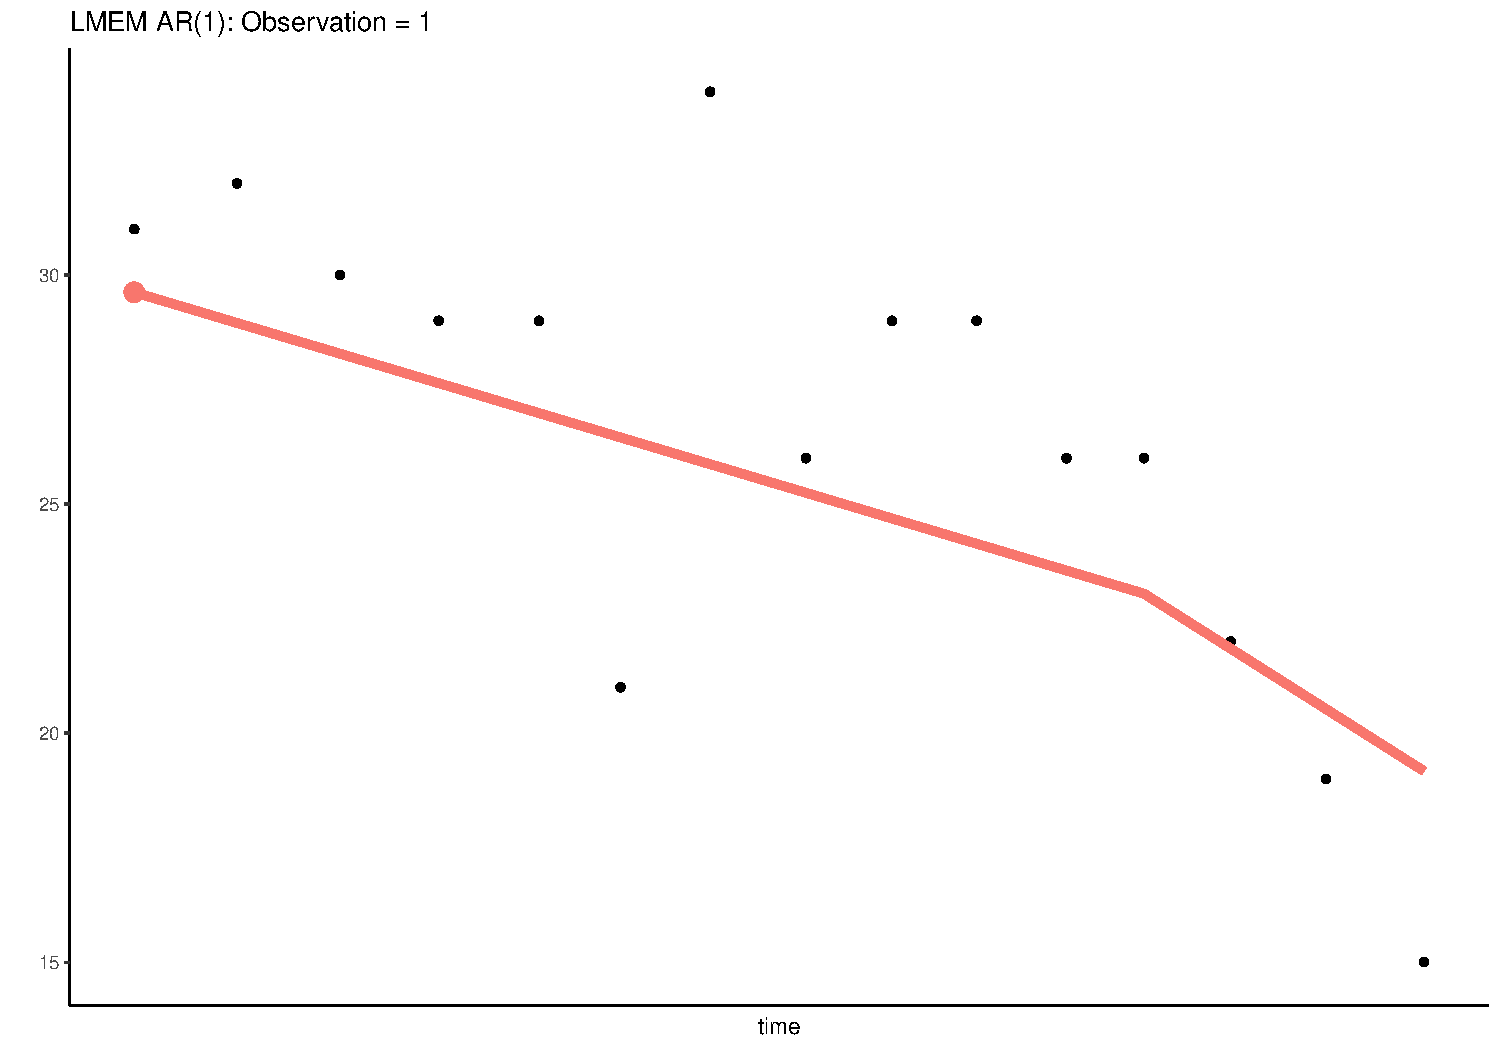
\includegraphics{Prez4_files/figure-beamer/unnamed-chunk-14-1.pdf}
\end{frame}

\begin{frame}{}
\protect\hypertarget{section-16}{}
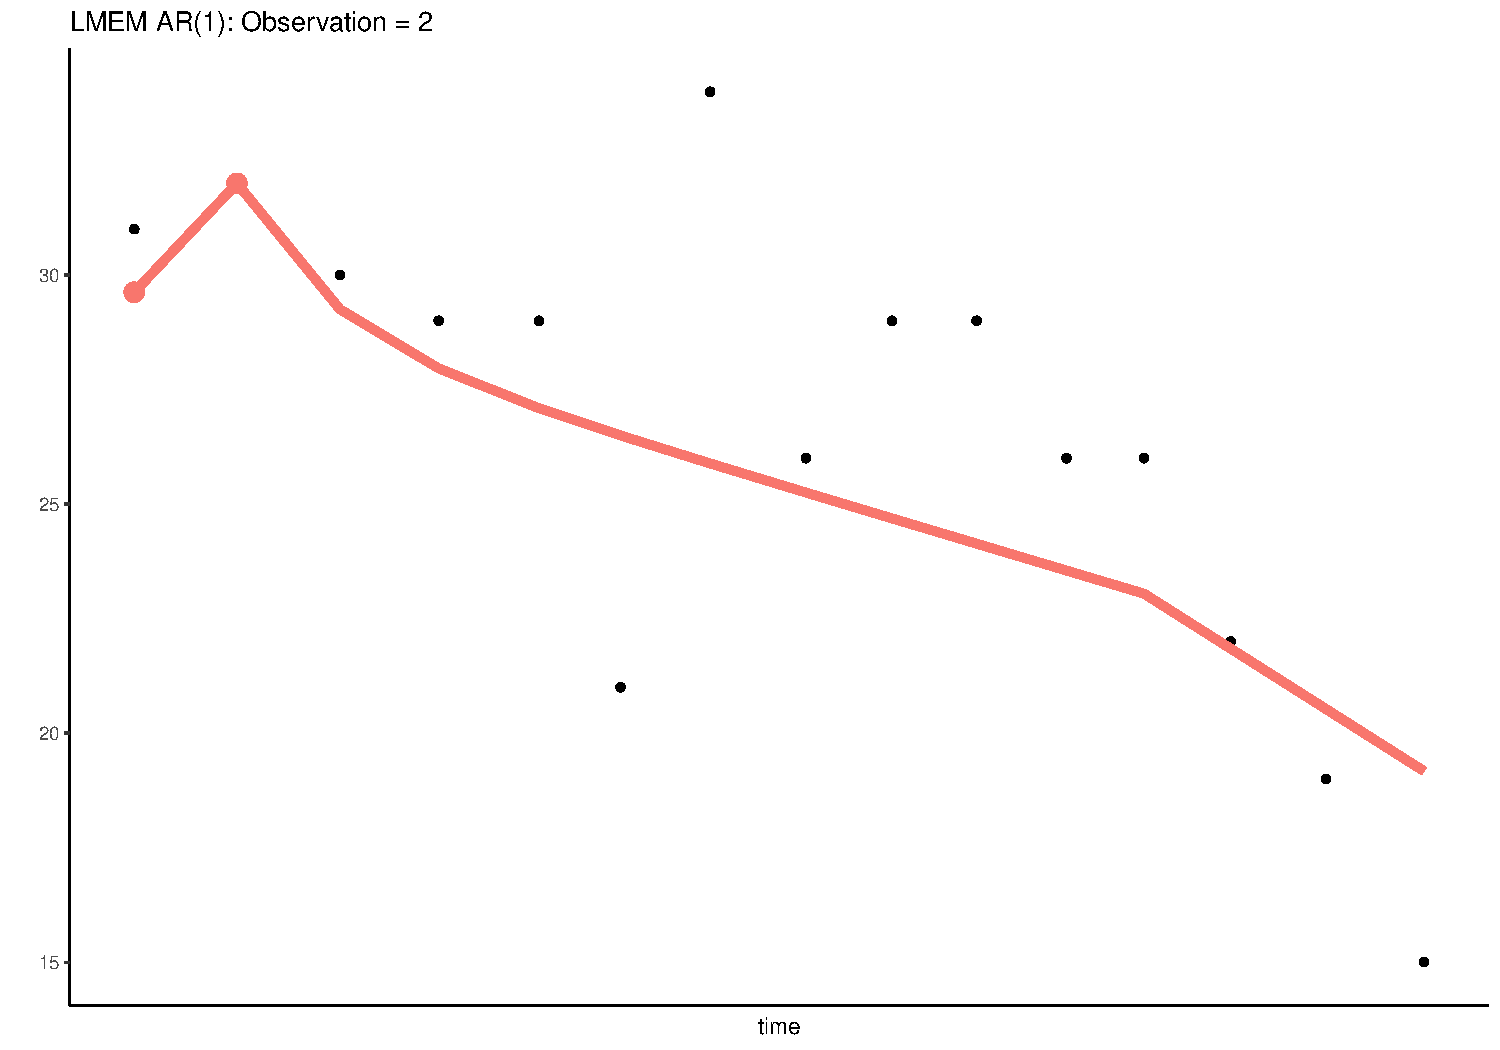
\includegraphics{Prez4_files/figure-beamer/unnamed-chunk-14-2.pdf}
\end{frame}

\begin{frame}{}
\protect\hypertarget{section-17}{}
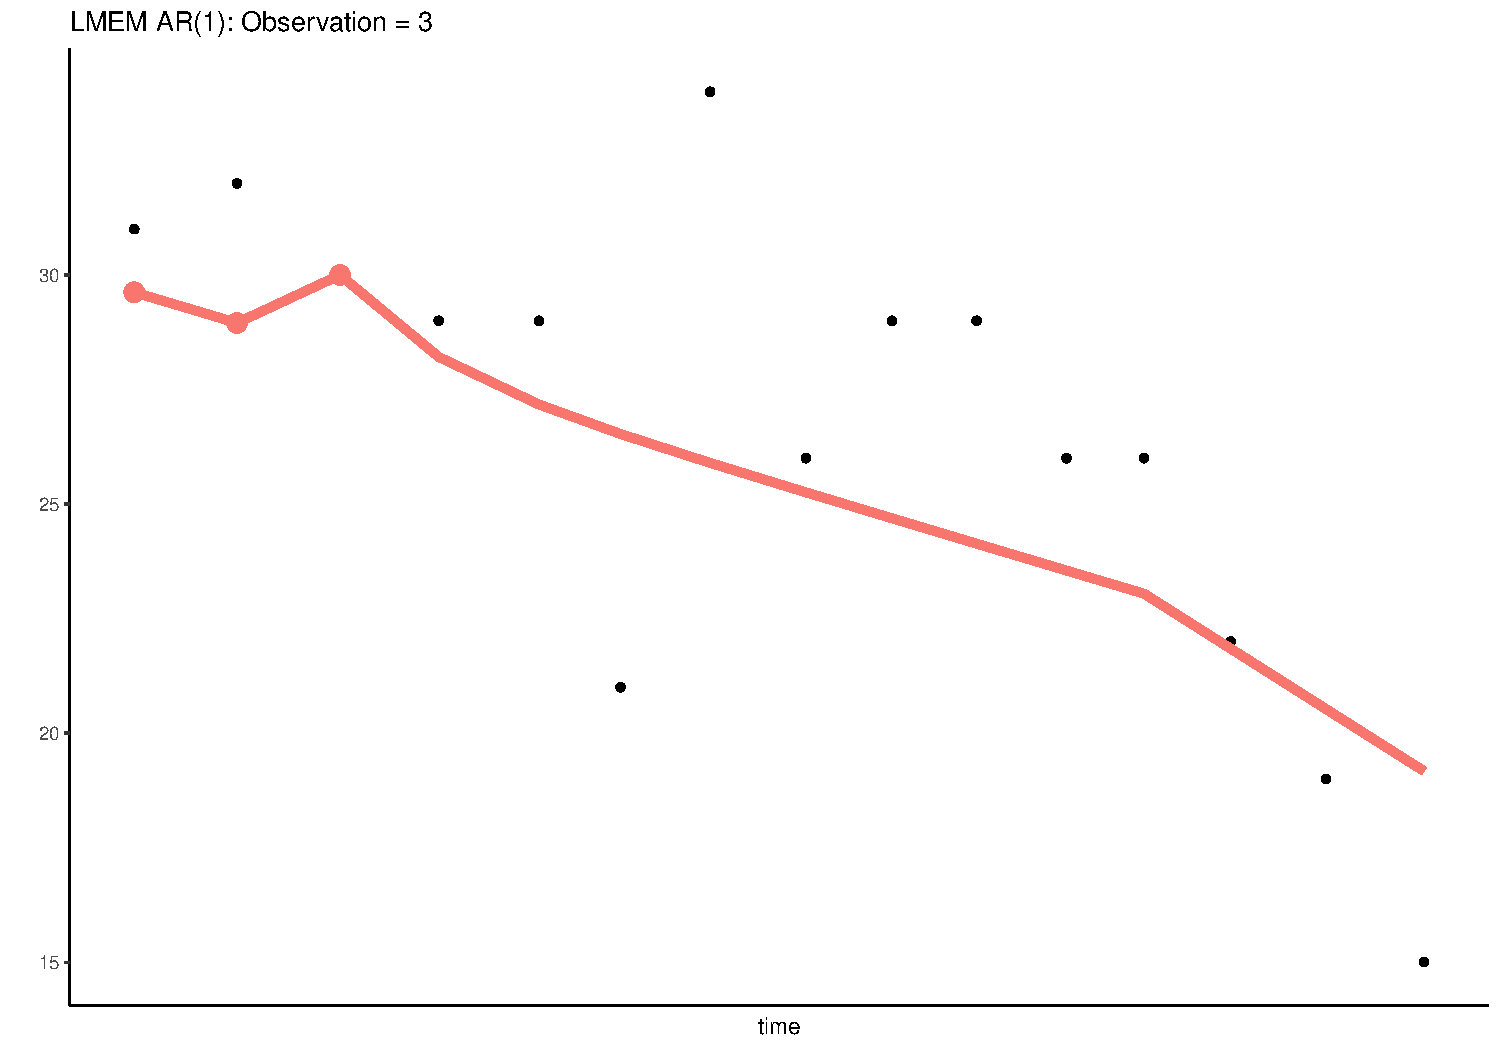
\includegraphics{Prez4_files/figure-beamer/unnamed-chunk-14-3.pdf}
\end{frame}

\begin{frame}{}
\protect\hypertarget{section-18}{}
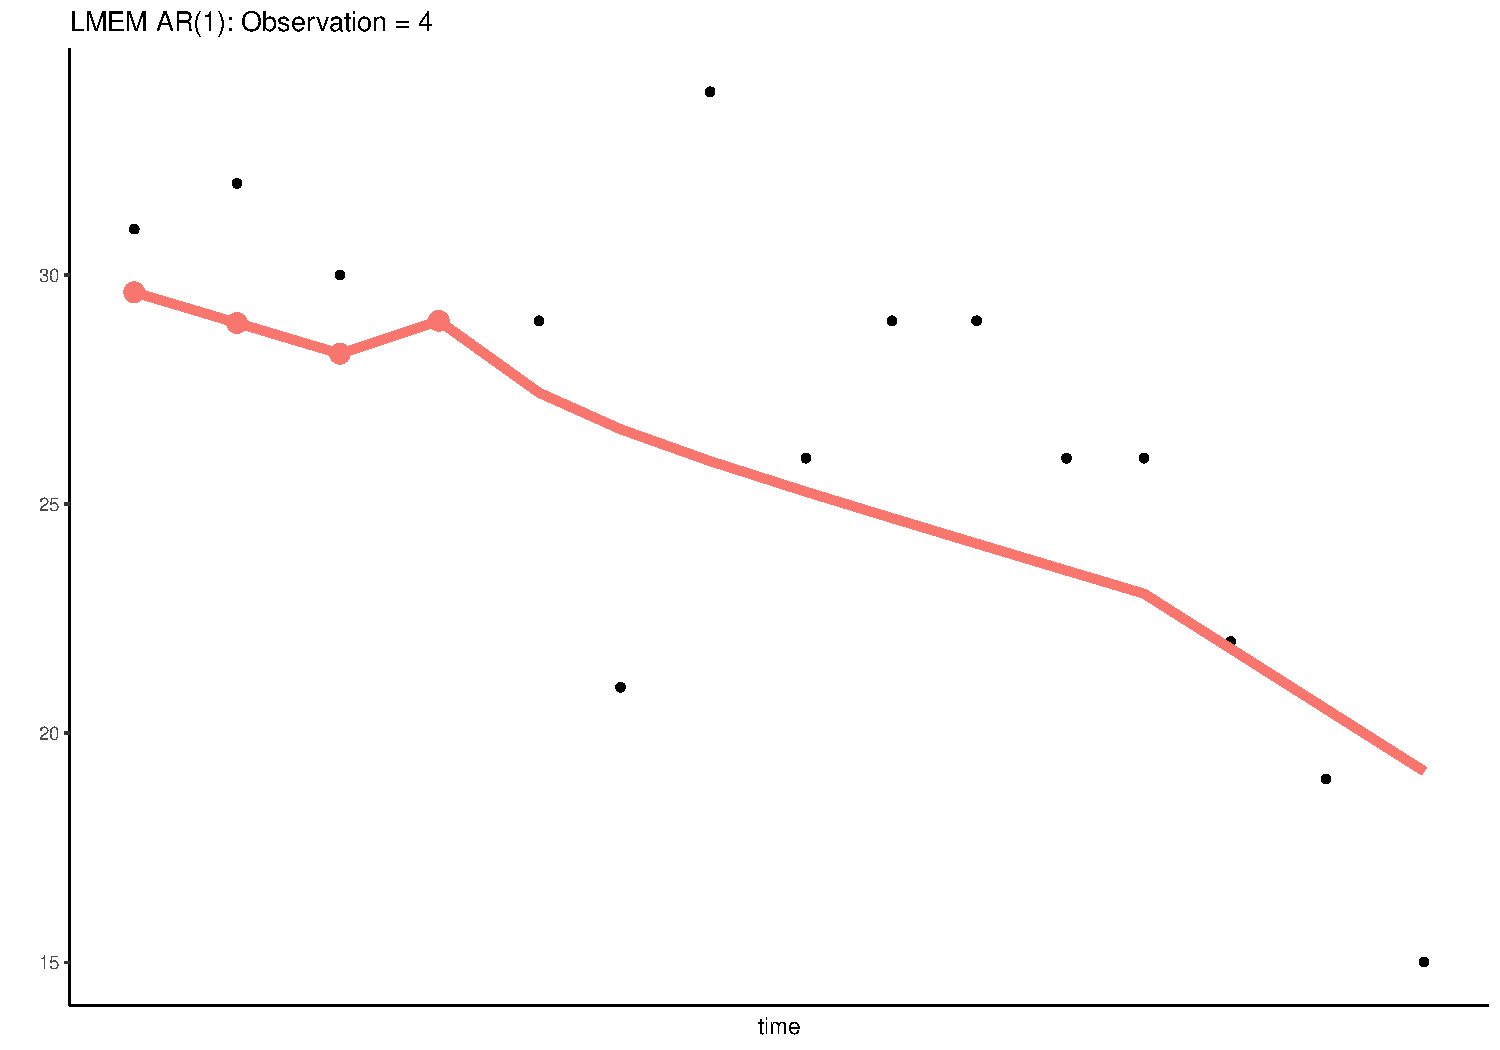
\includegraphics{Prez4_files/figure-beamer/unnamed-chunk-14-4.pdf}
\end{frame}

\begin{frame}{}
\protect\hypertarget{section-19}{}
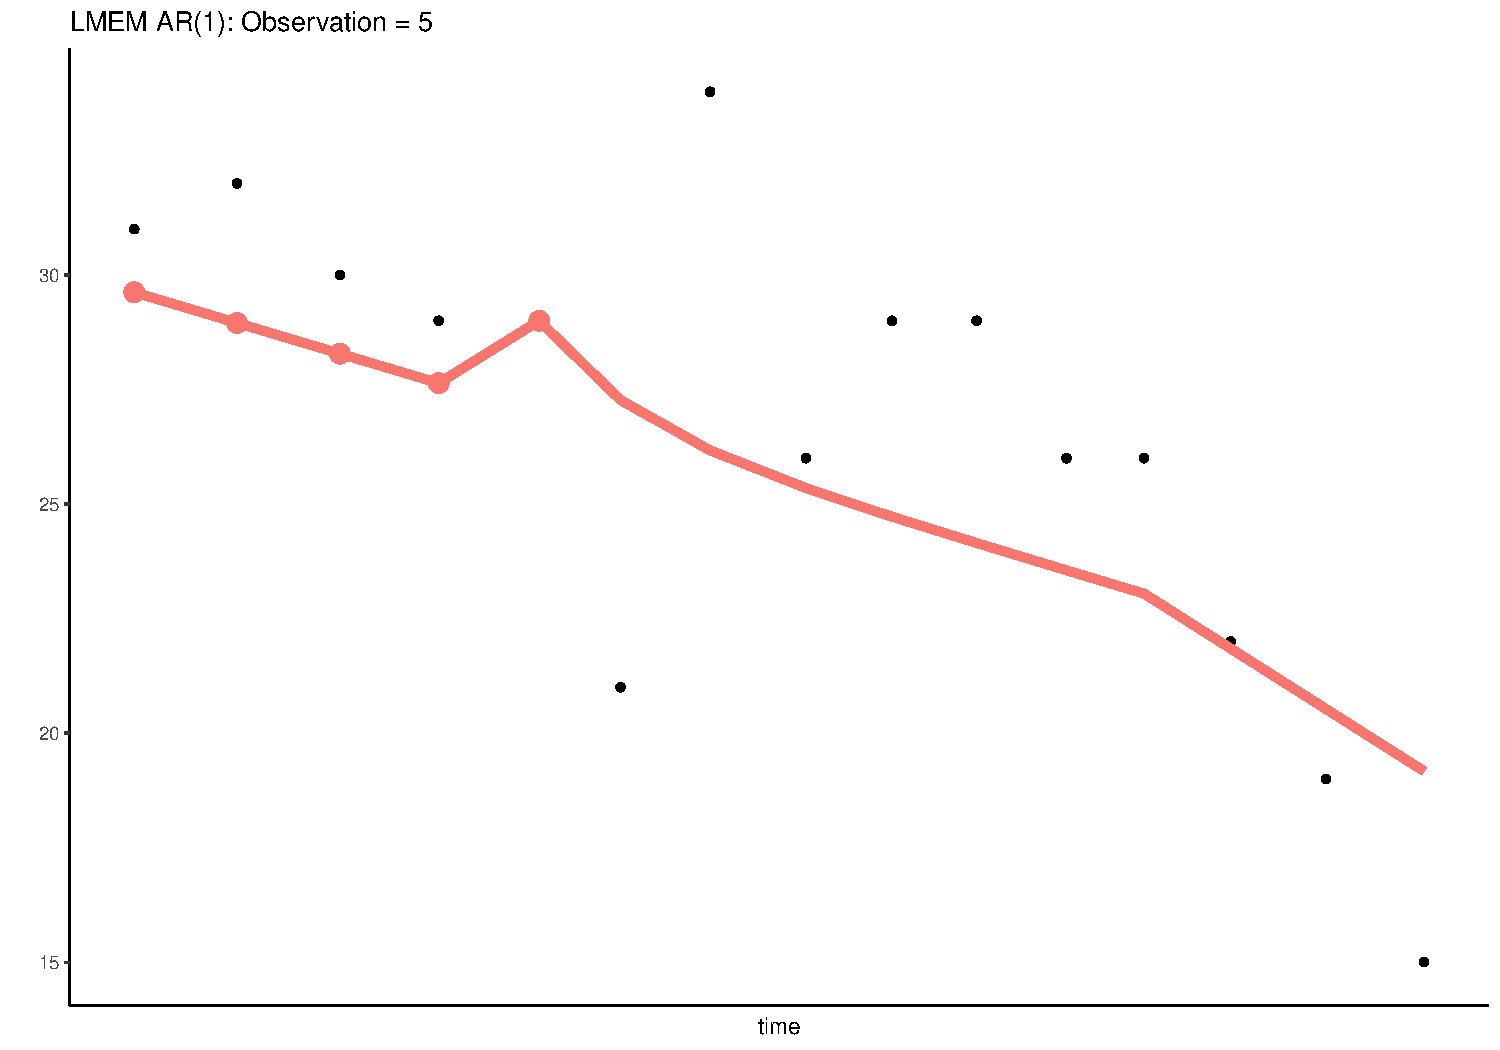
\includegraphics{Prez4_files/figure-beamer/unnamed-chunk-14-5.pdf}
\end{frame}

\begin{frame}{}
\protect\hypertarget{section-20}{}
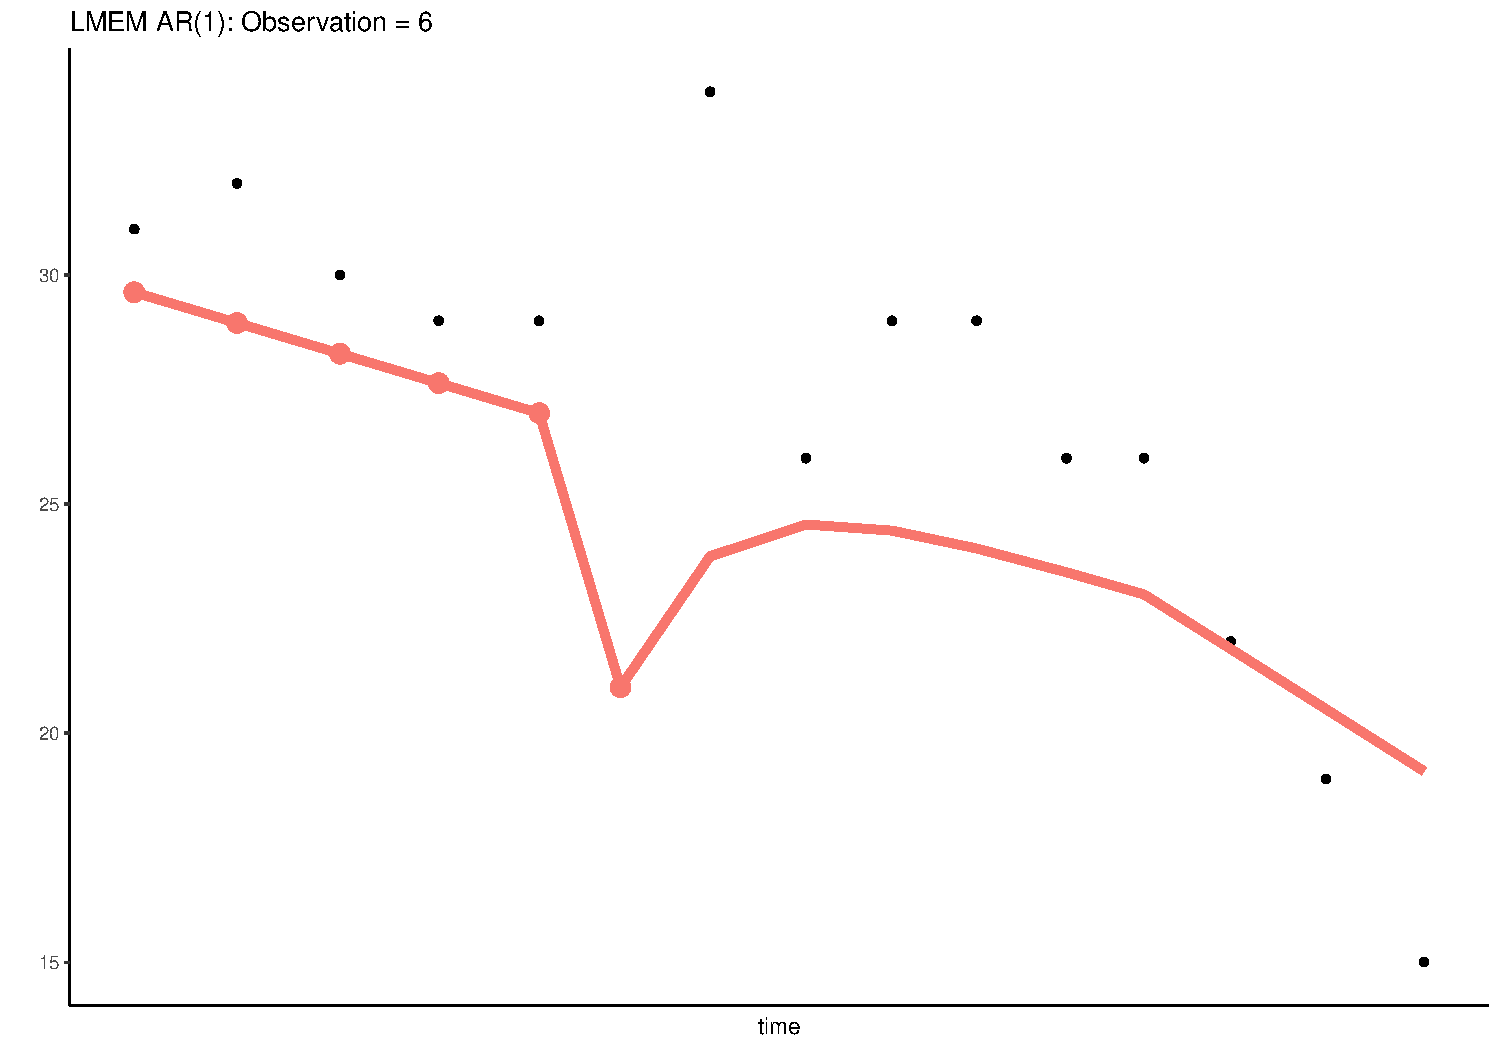
\includegraphics{Prez4_files/figure-beamer/unnamed-chunk-14-6.pdf}
\end{frame}

\begin{frame}{}
\protect\hypertarget{section-21}{}
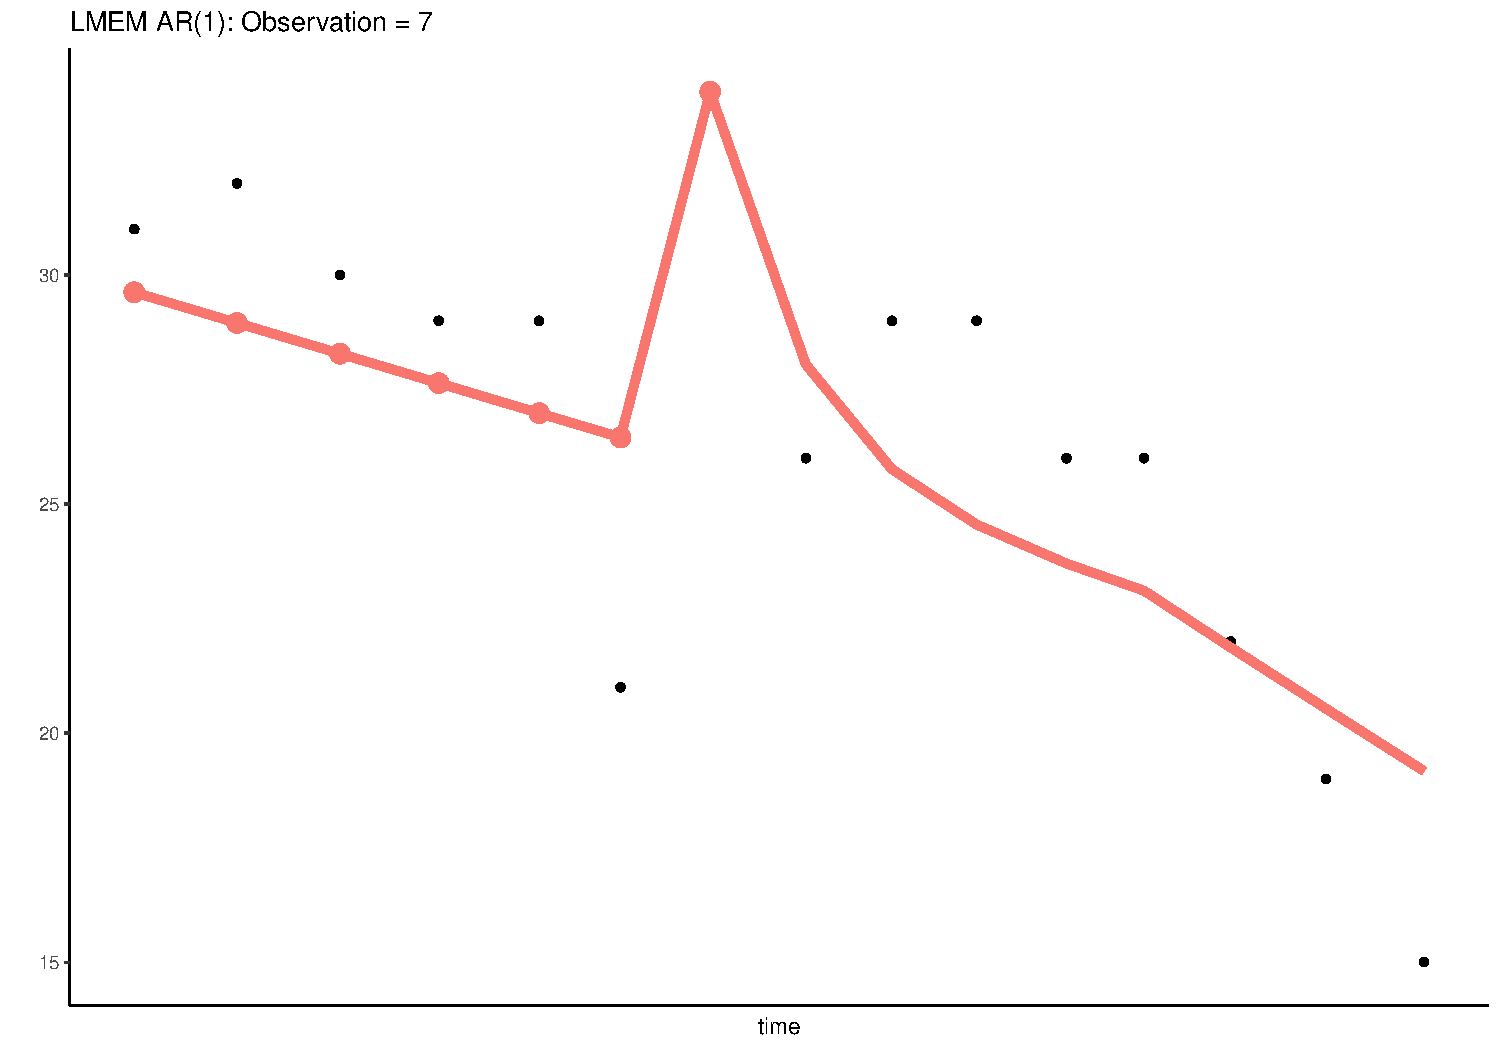
\includegraphics{Prez4_files/figure-beamer/unnamed-chunk-14-7.pdf}
\end{frame}

\begin{frame}{}
\protect\hypertarget{section-22}{}
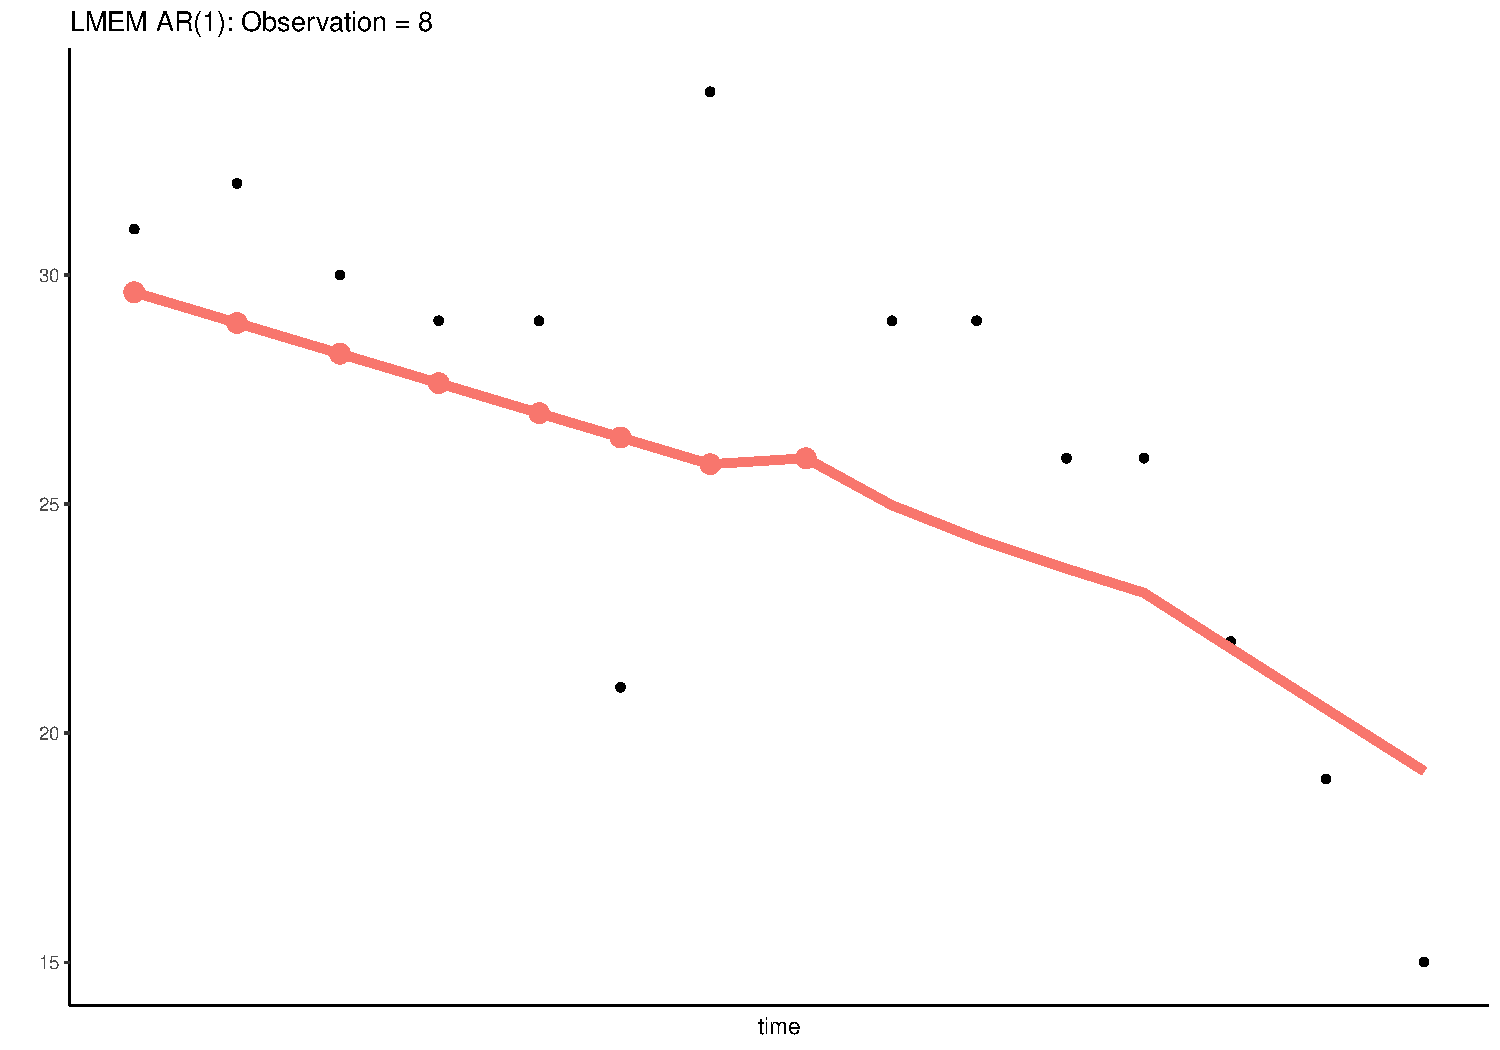
\includegraphics{Prez4_files/figure-beamer/unnamed-chunk-14-8.pdf}
\end{frame}

\begin{frame}{}
\protect\hypertarget{section-23}{}
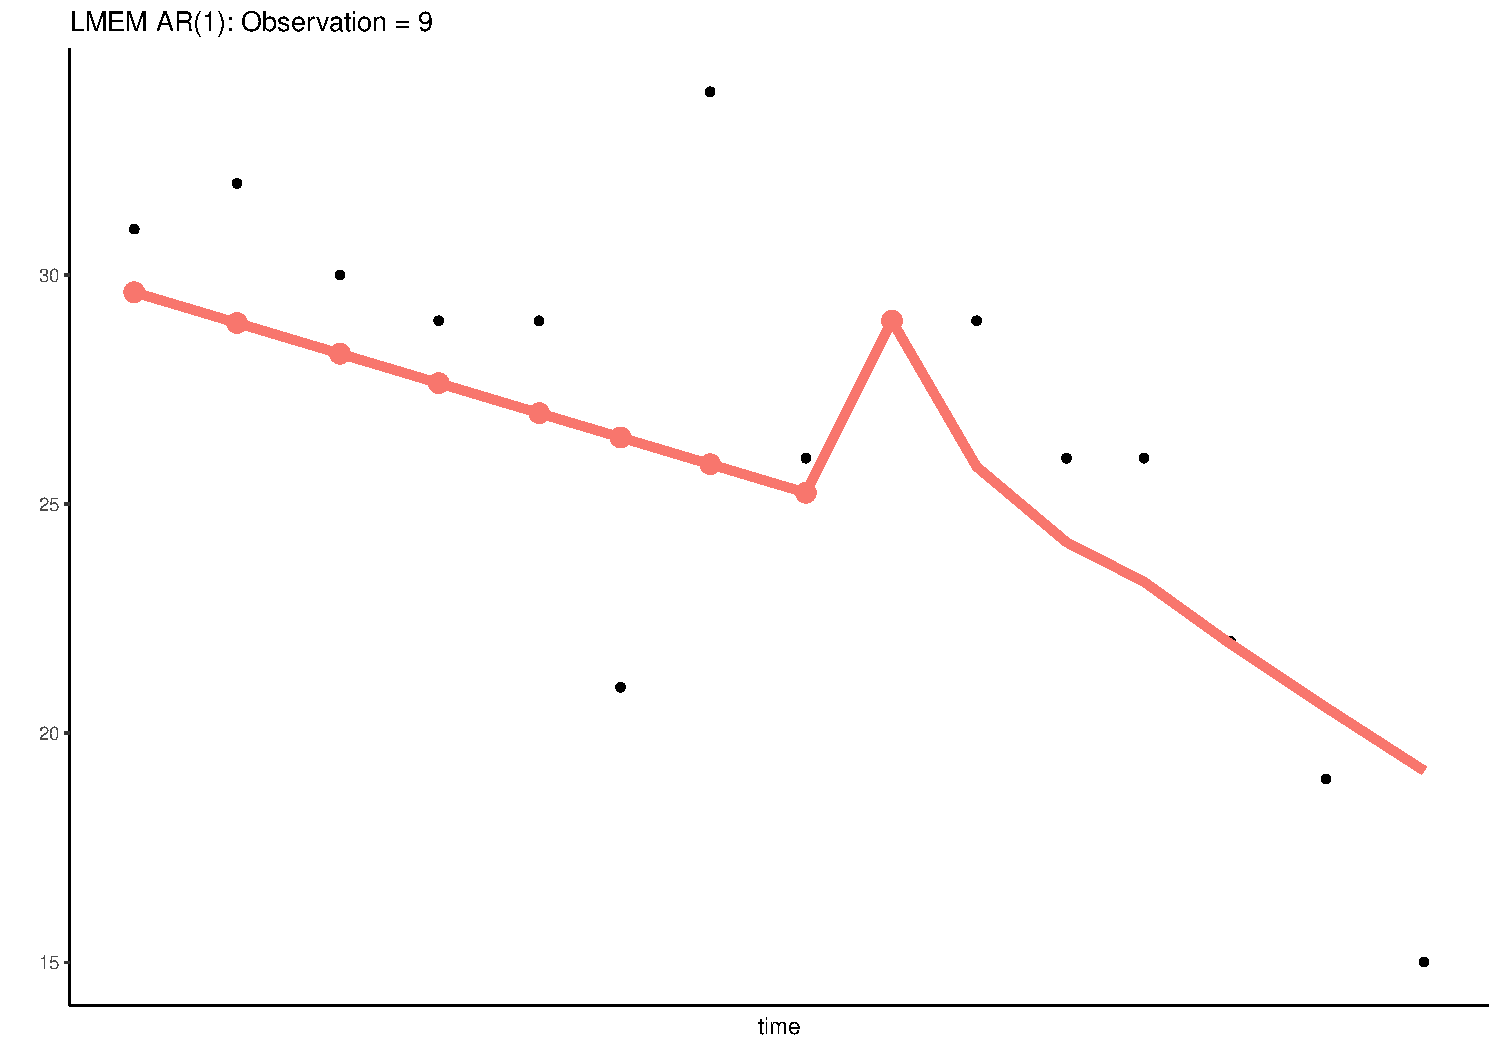
\includegraphics{Prez4_files/figure-beamer/unnamed-chunk-14-9.pdf}
\end{frame}

\begin{frame}{}
\protect\hypertarget{section-24}{}
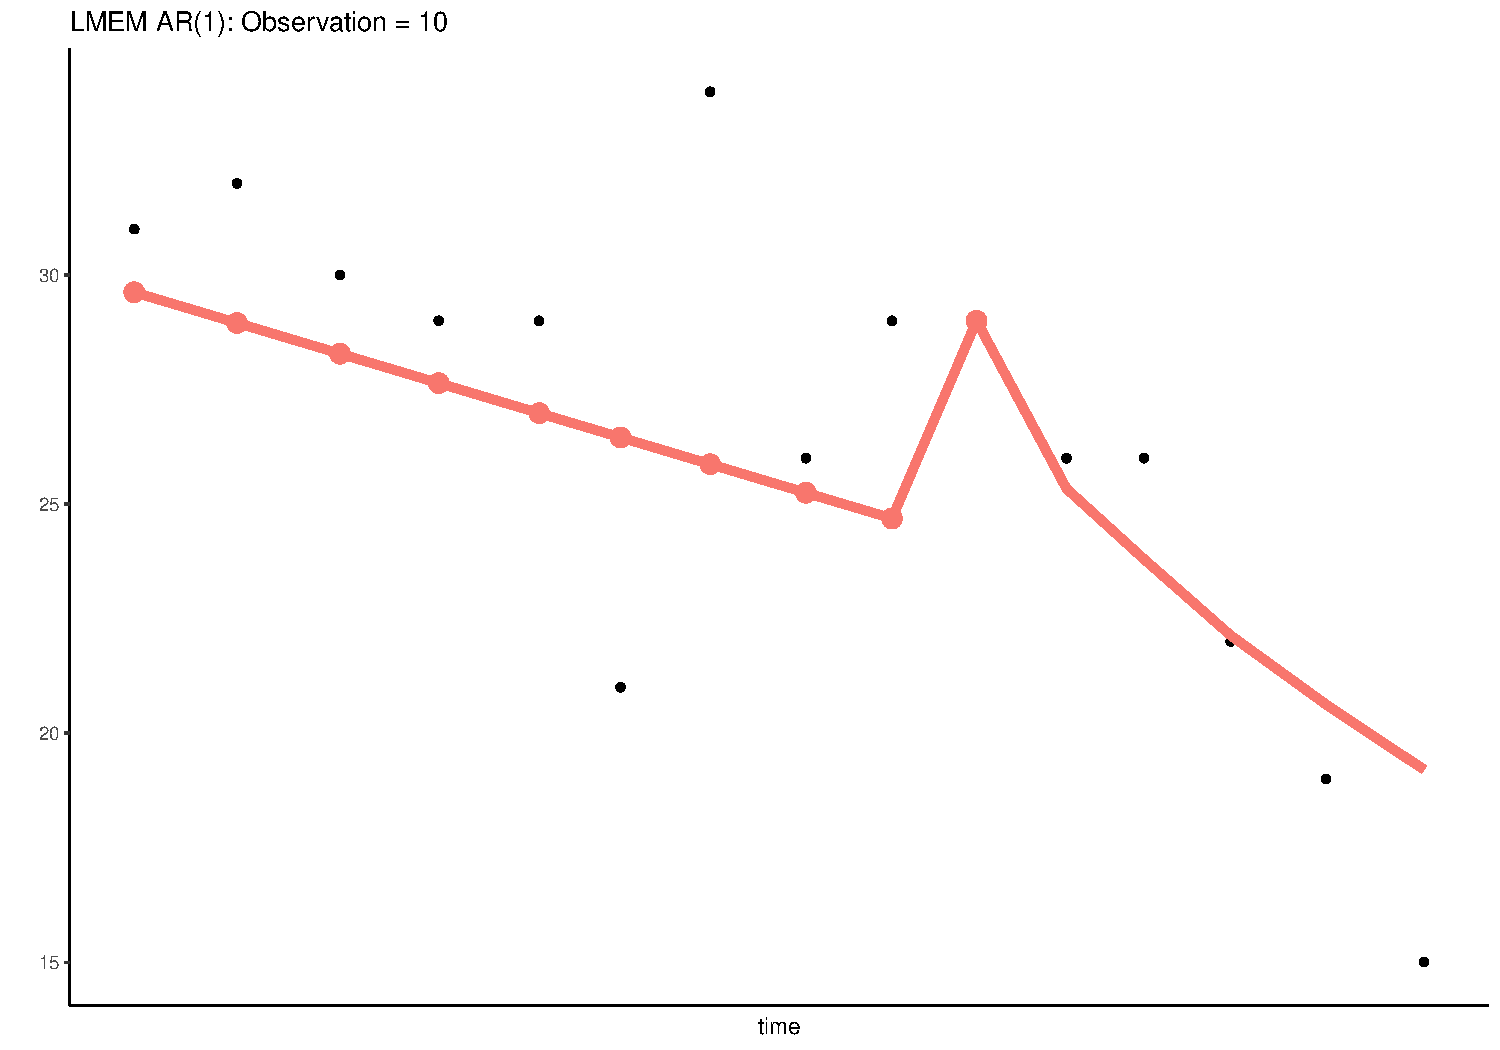
\includegraphics{Prez4_files/figure-beamer/unnamed-chunk-14-10.pdf}
\end{frame}

\begin{frame}{}
\protect\hypertarget{section-25}{}
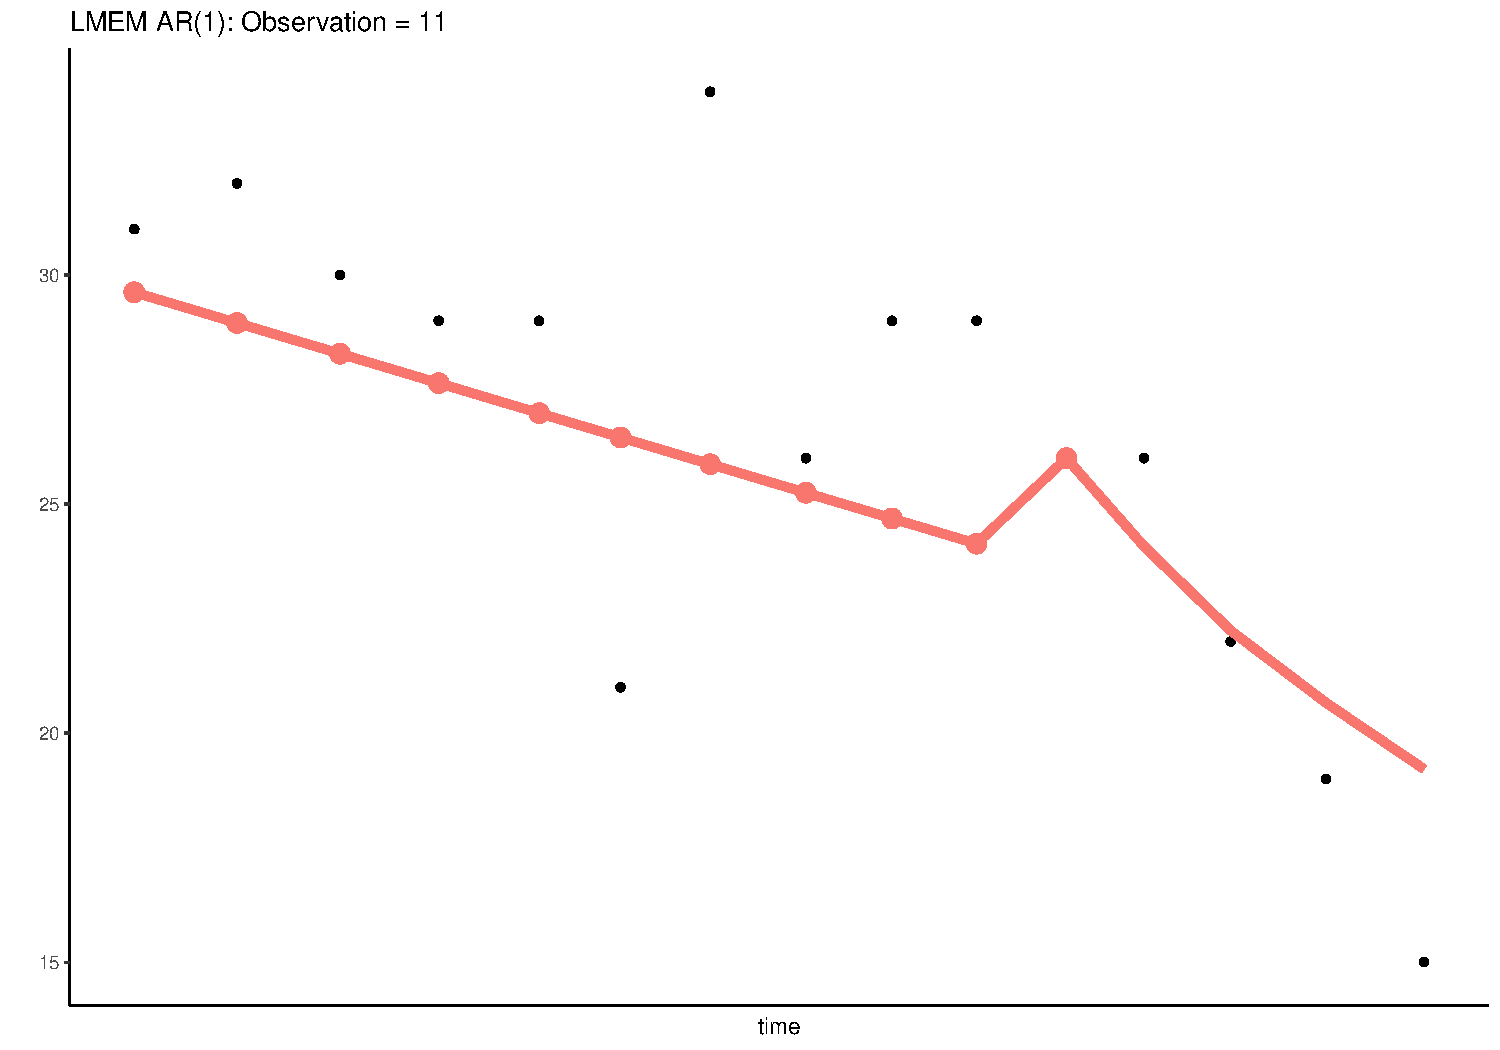
\includegraphics{Prez4_files/figure-beamer/unnamed-chunk-14-11.pdf}
\end{frame}

\begin{frame}{}
\protect\hypertarget{section-26}{}
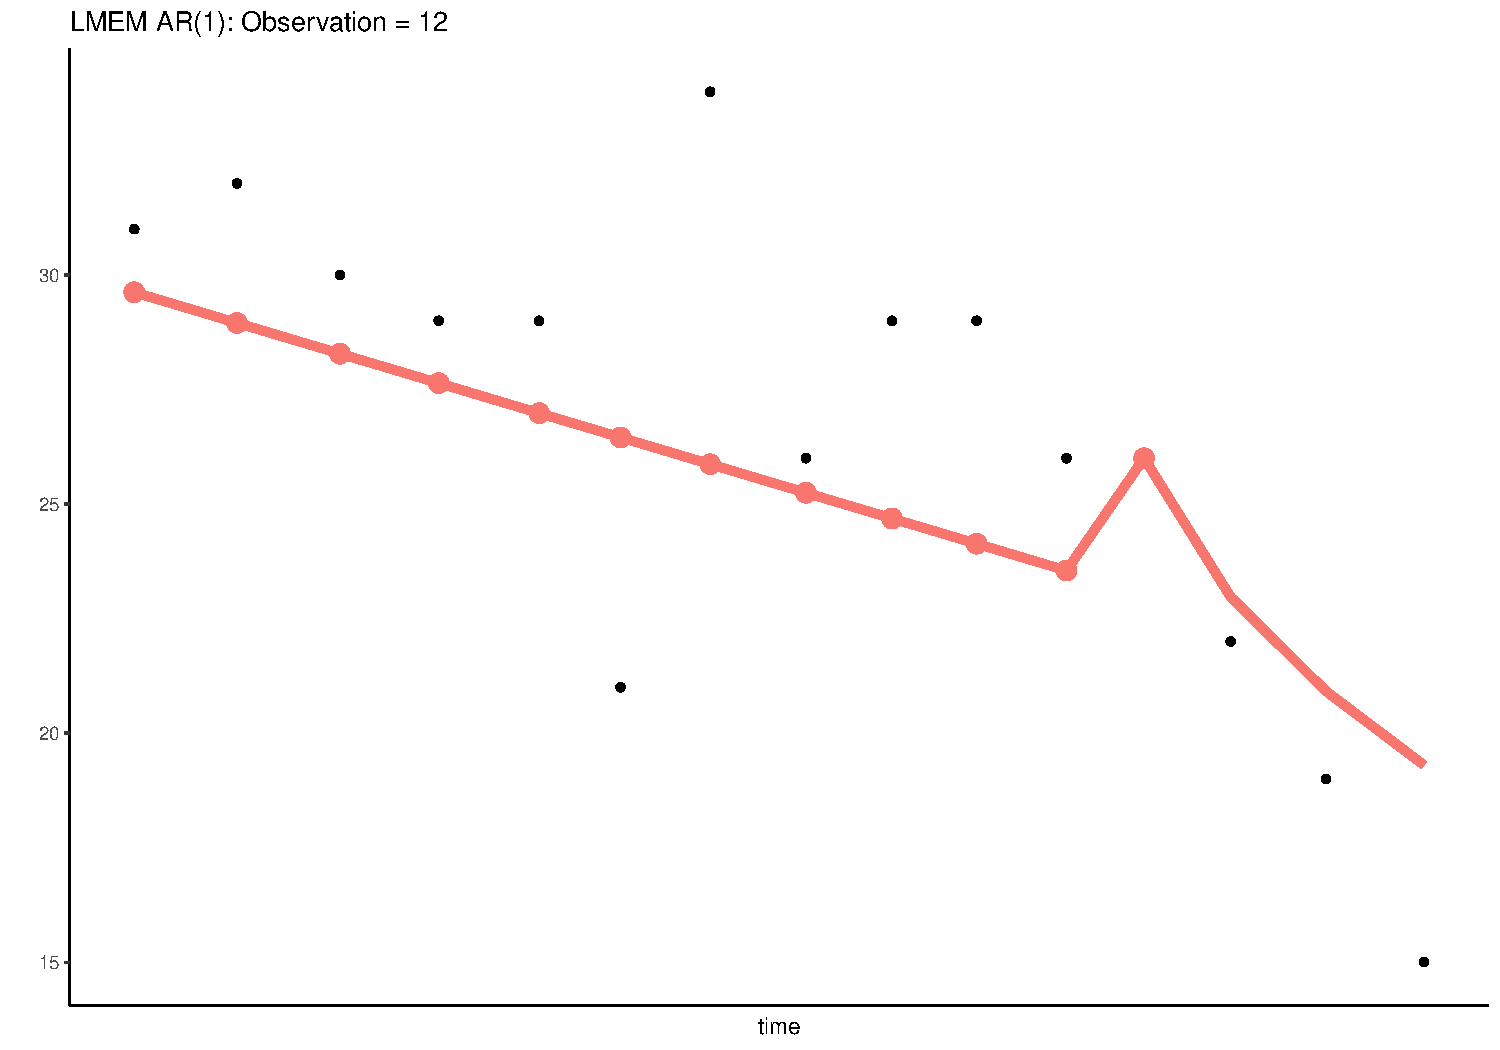
\includegraphics{Prez4_files/figure-beamer/unnamed-chunk-14-12.pdf}
\end{frame}

\begin{frame}{}
\protect\hypertarget{section-27}{}
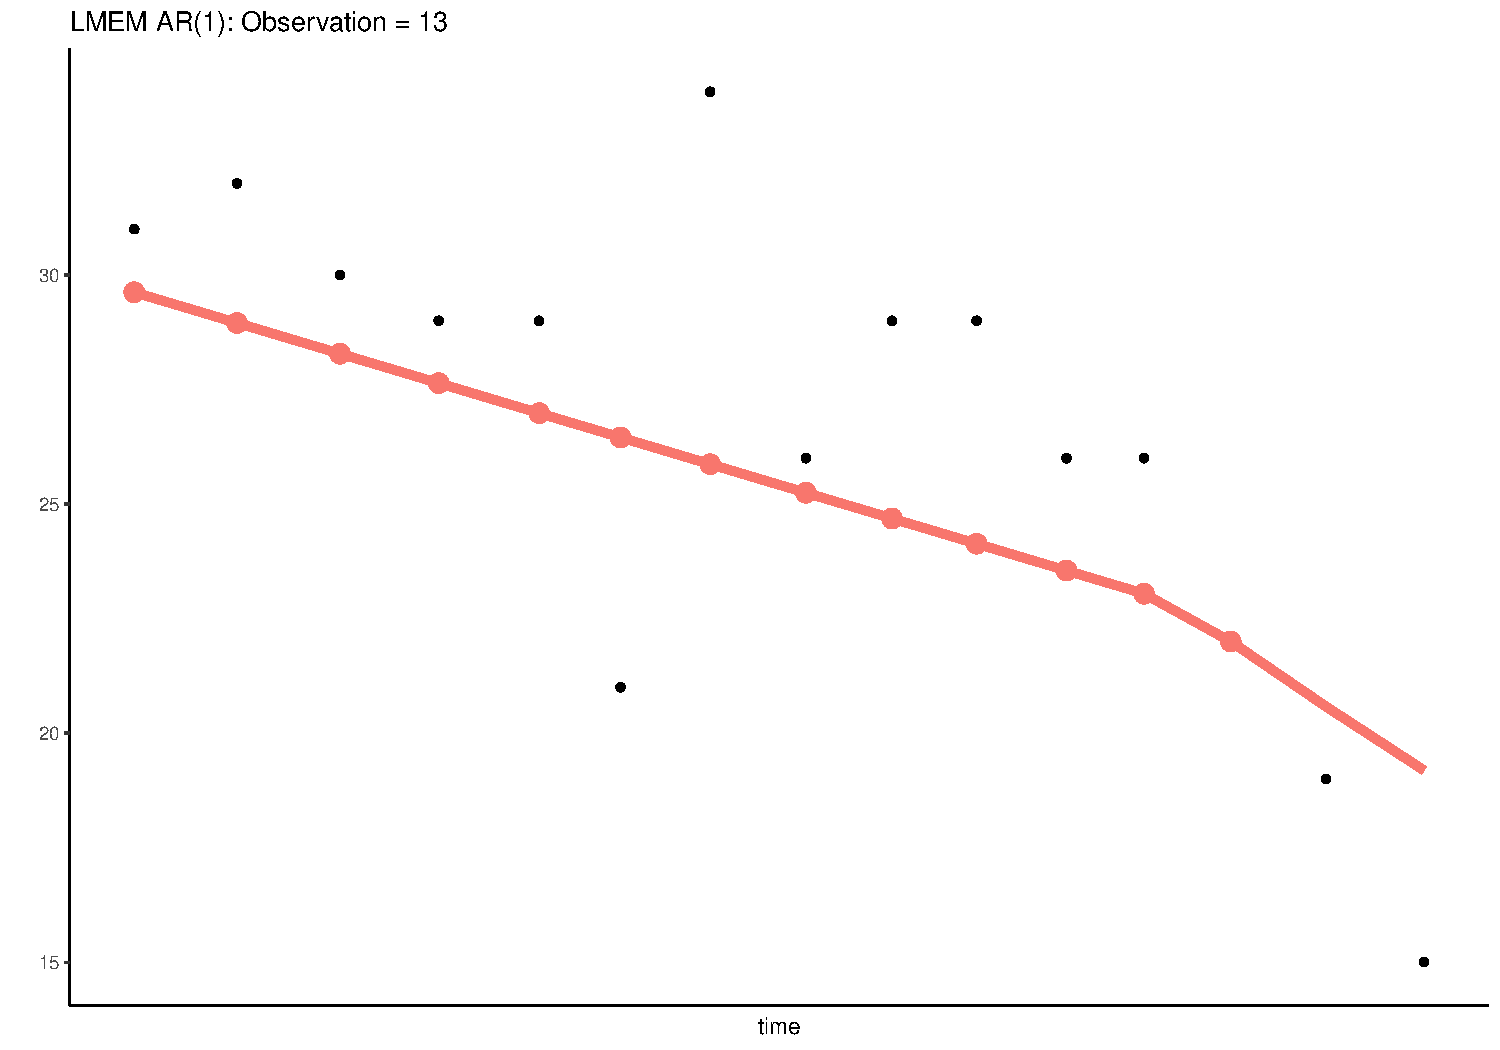
\includegraphics{Prez4_files/figure-beamer/unnamed-chunk-14-13.pdf}
\end{frame}

\begin{frame}{}
\protect\hypertarget{section-28}{}
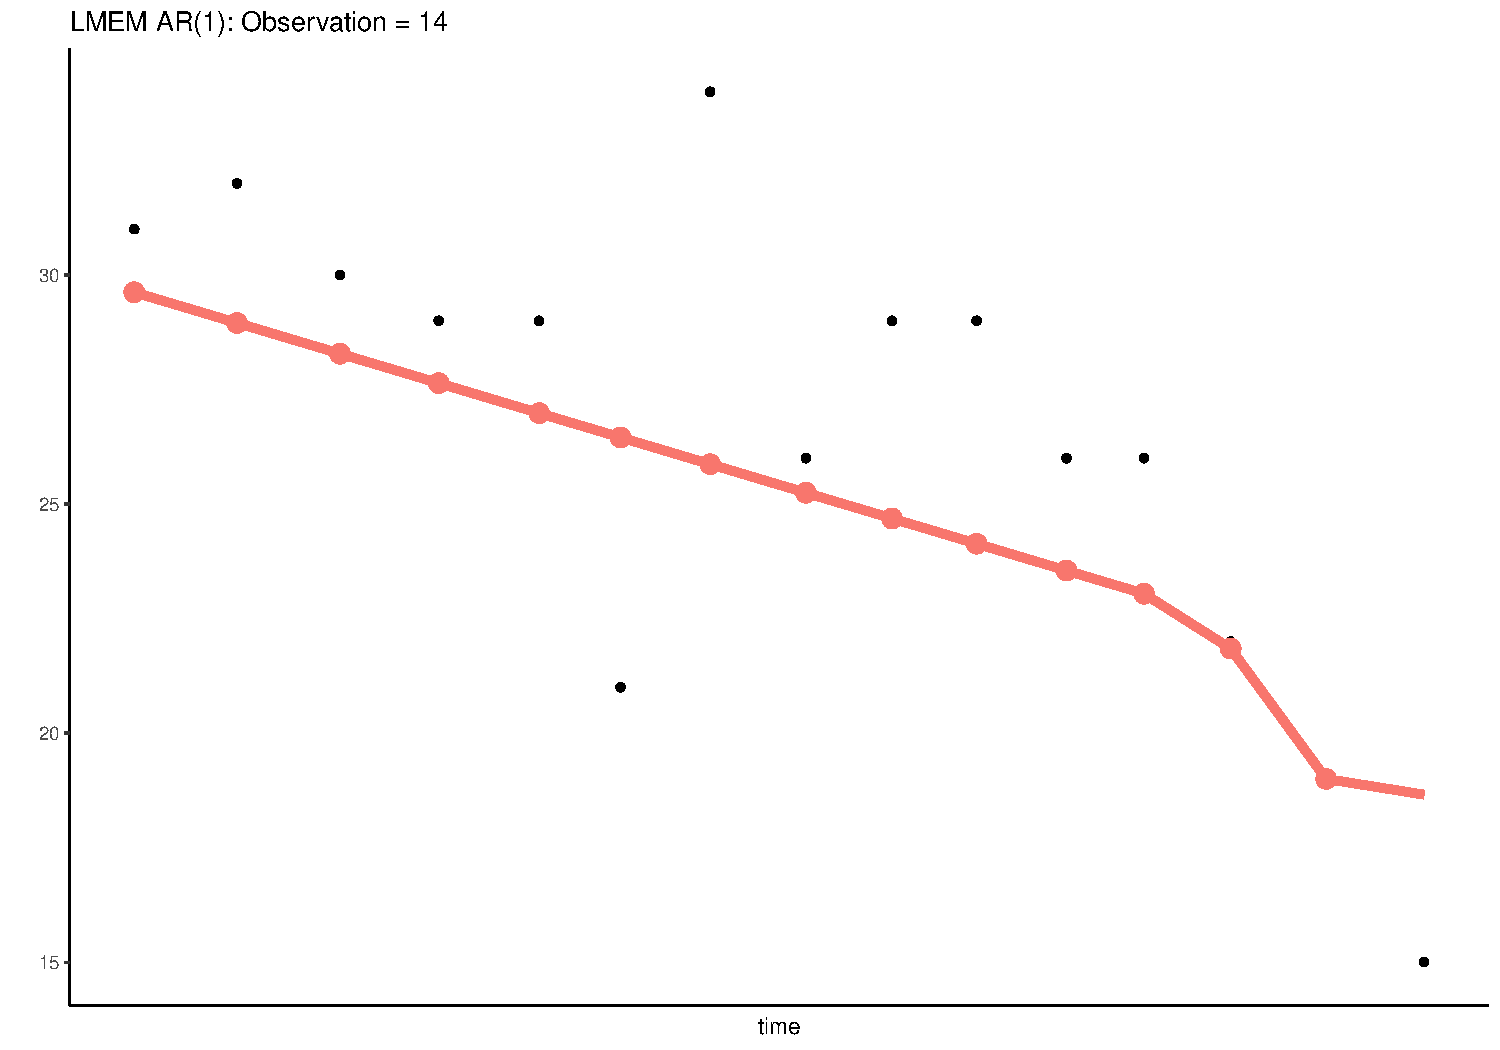
\includegraphics{Prez4_files/figure-beamer/unnamed-chunk-14-14.pdf}
\end{frame}

\begin{frame}{}
\protect\hypertarget{section-29}{}
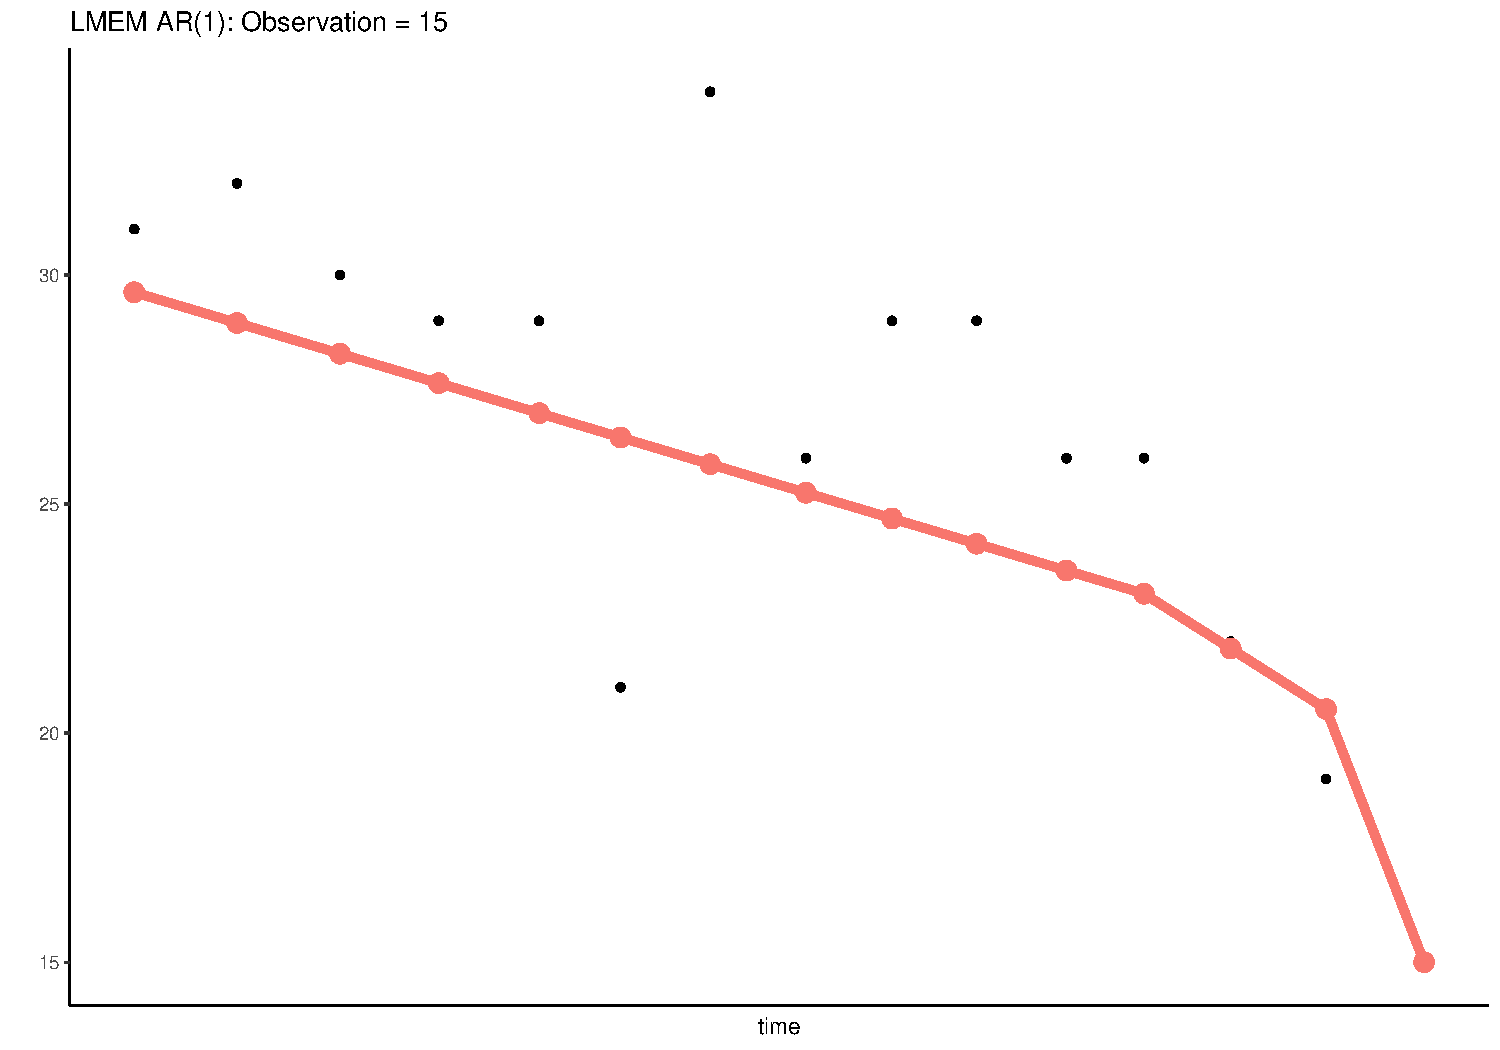
\includegraphics{Prez4_files/figure-beamer/unnamed-chunk-14-15.pdf}
\end{frame}

\begin{frame}{}
\protect\hypertarget{section-30}{}
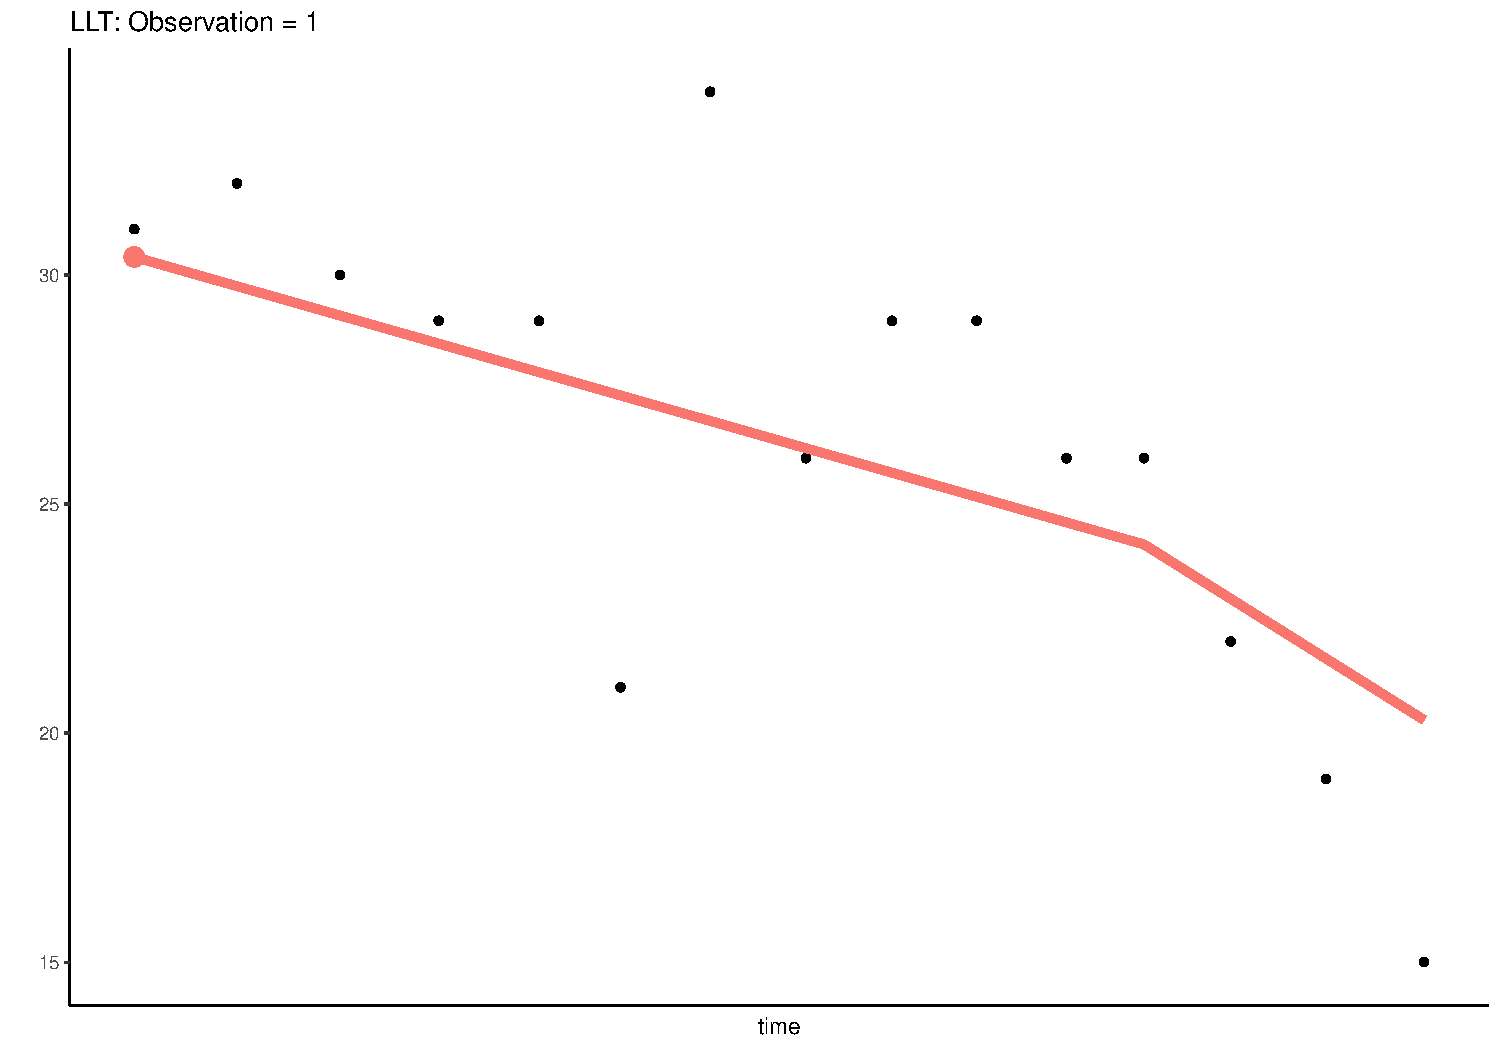
\includegraphics{Prez4_files/figure-beamer/unnamed-chunk-15-1.pdf}
\end{frame}

\begin{frame}{}
\protect\hypertarget{section-31}{}
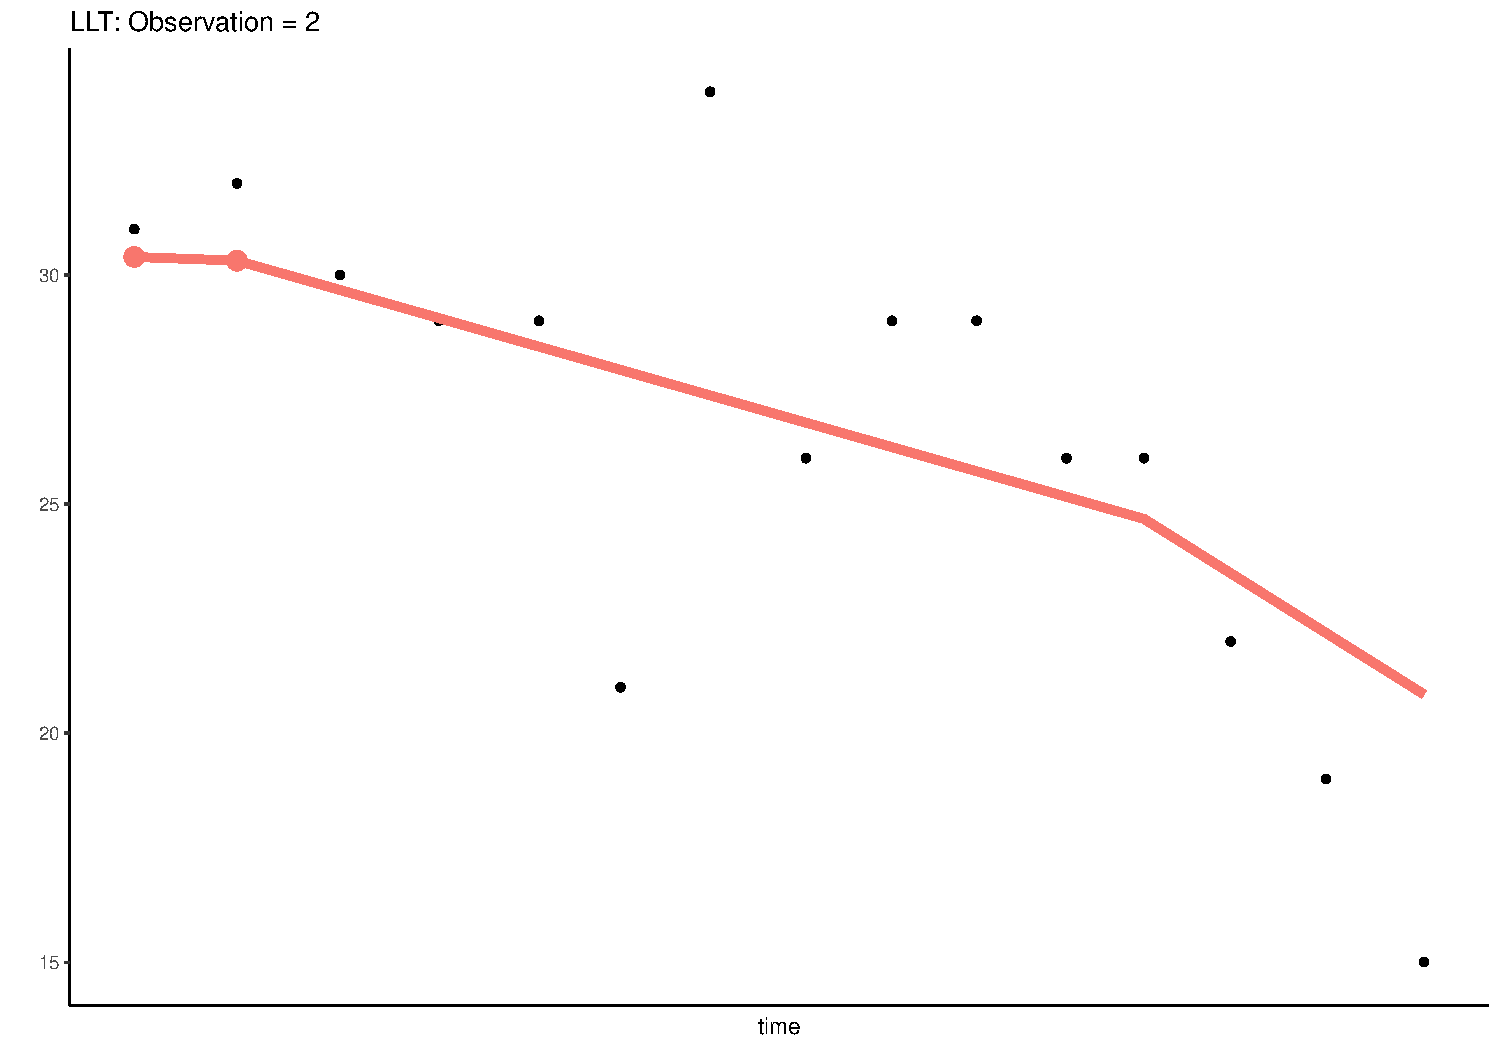
\includegraphics{Prez4_files/figure-beamer/unnamed-chunk-15-2.pdf}
\end{frame}

\begin{frame}{}
\protect\hypertarget{section-32}{}
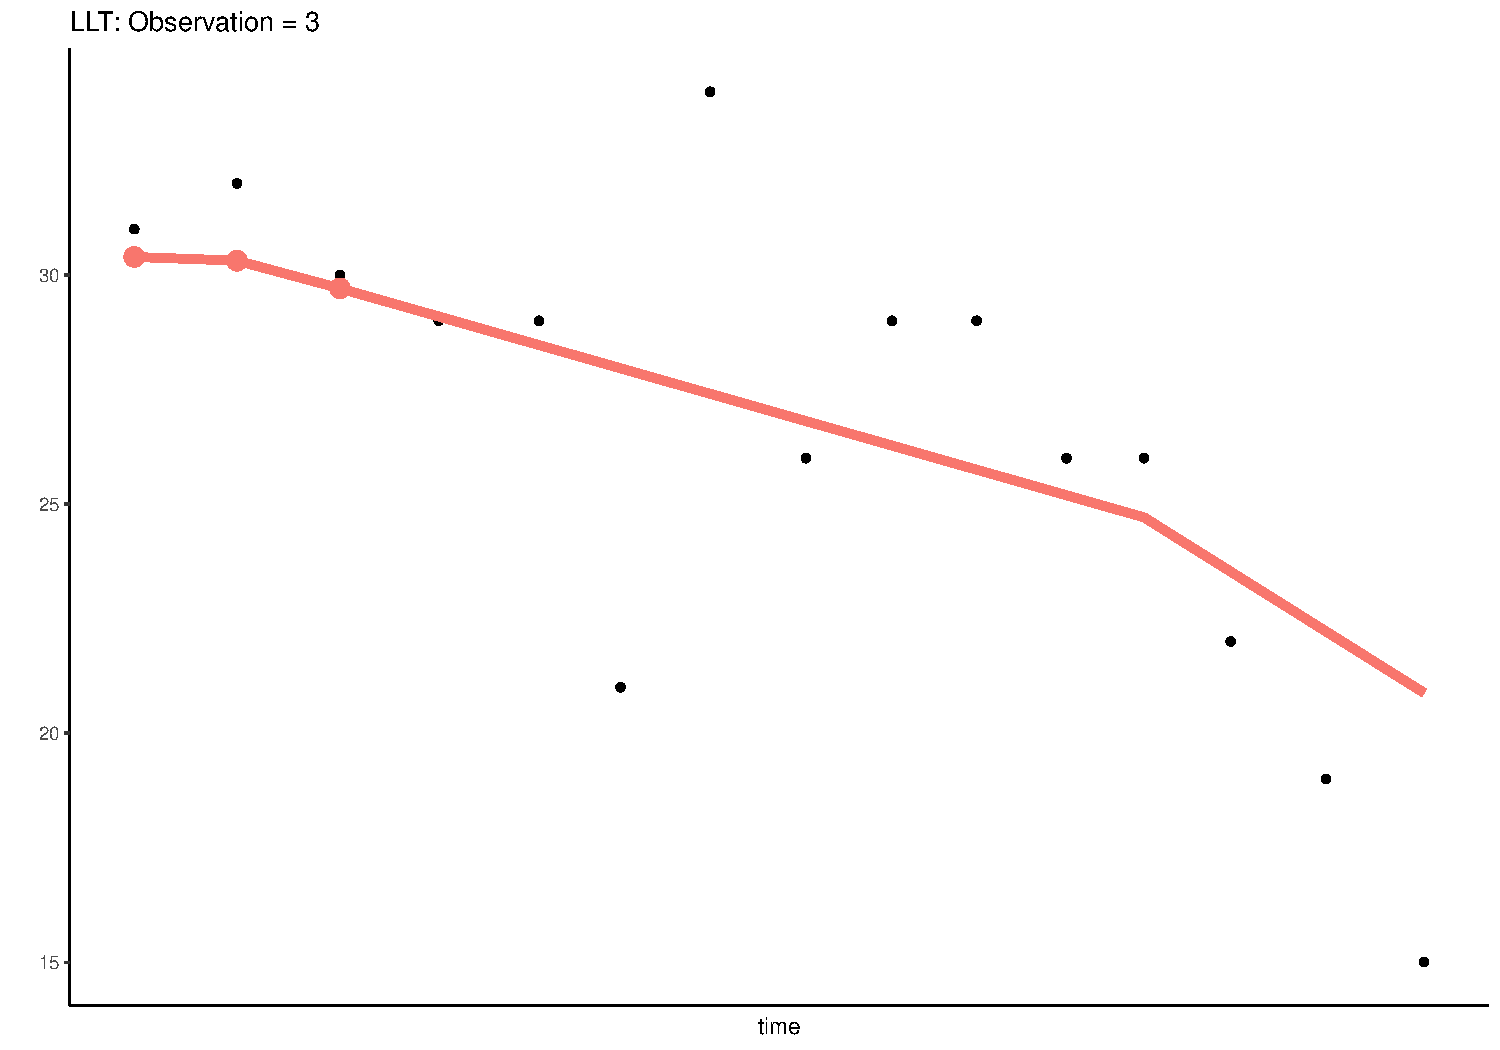
\includegraphics{Prez4_files/figure-beamer/unnamed-chunk-15-3.pdf}
\end{frame}

\begin{frame}{}
\protect\hypertarget{section-33}{}
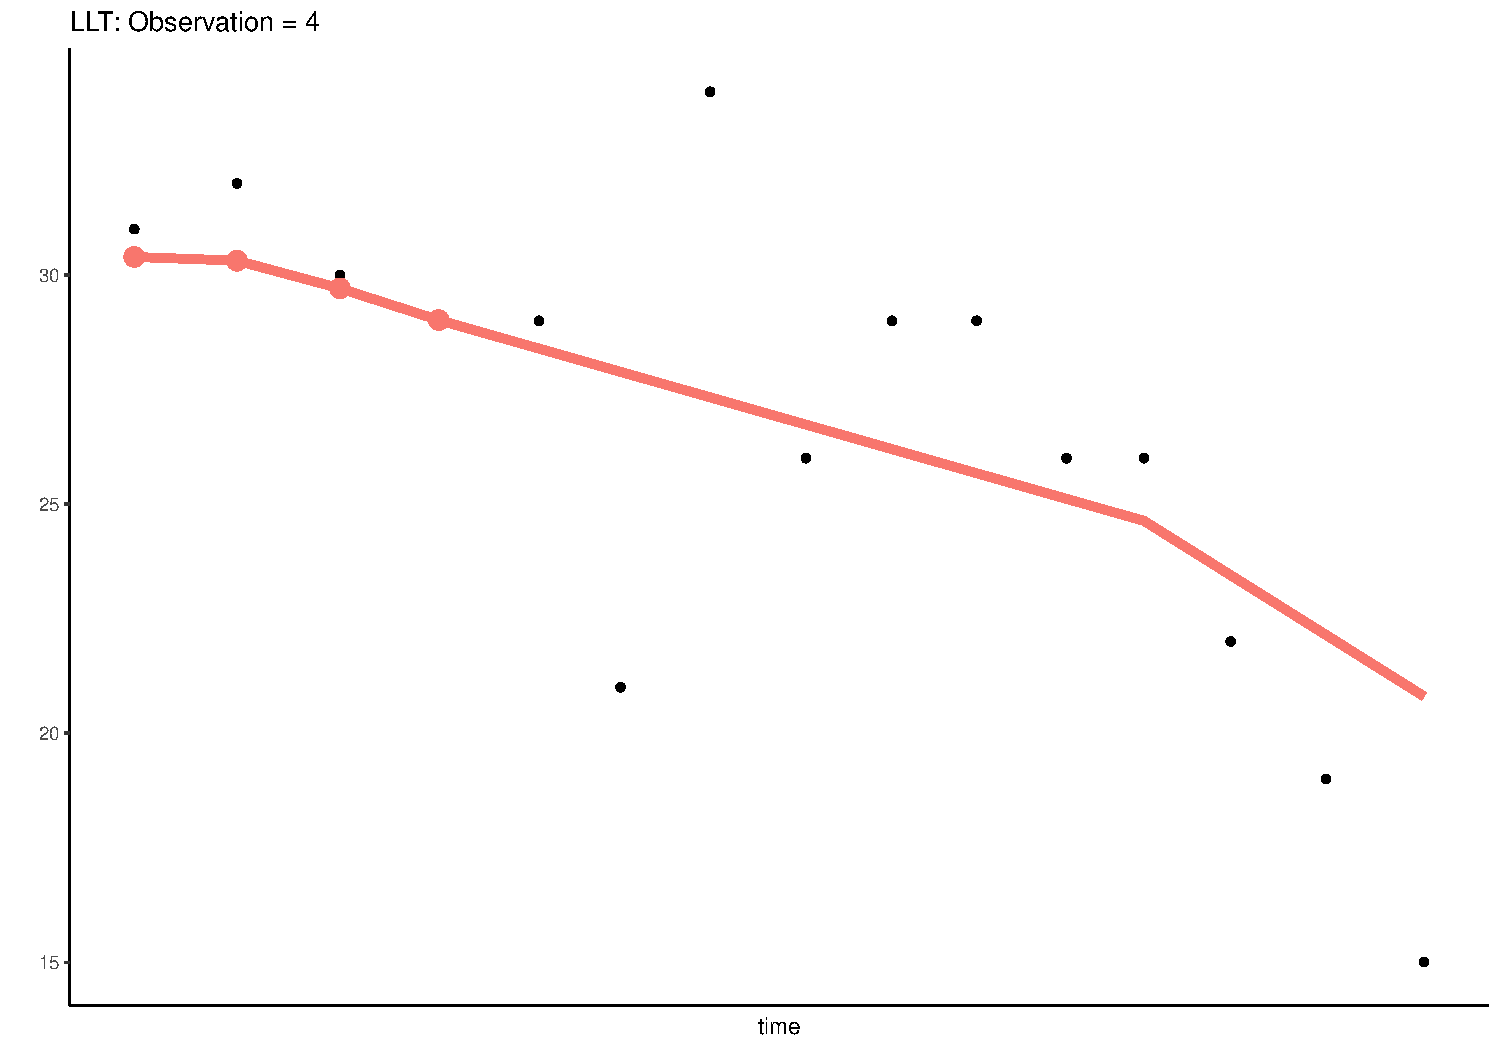
\includegraphics{Prez4_files/figure-beamer/unnamed-chunk-15-4.pdf}
\end{frame}

\begin{frame}{}
\protect\hypertarget{section-34}{}
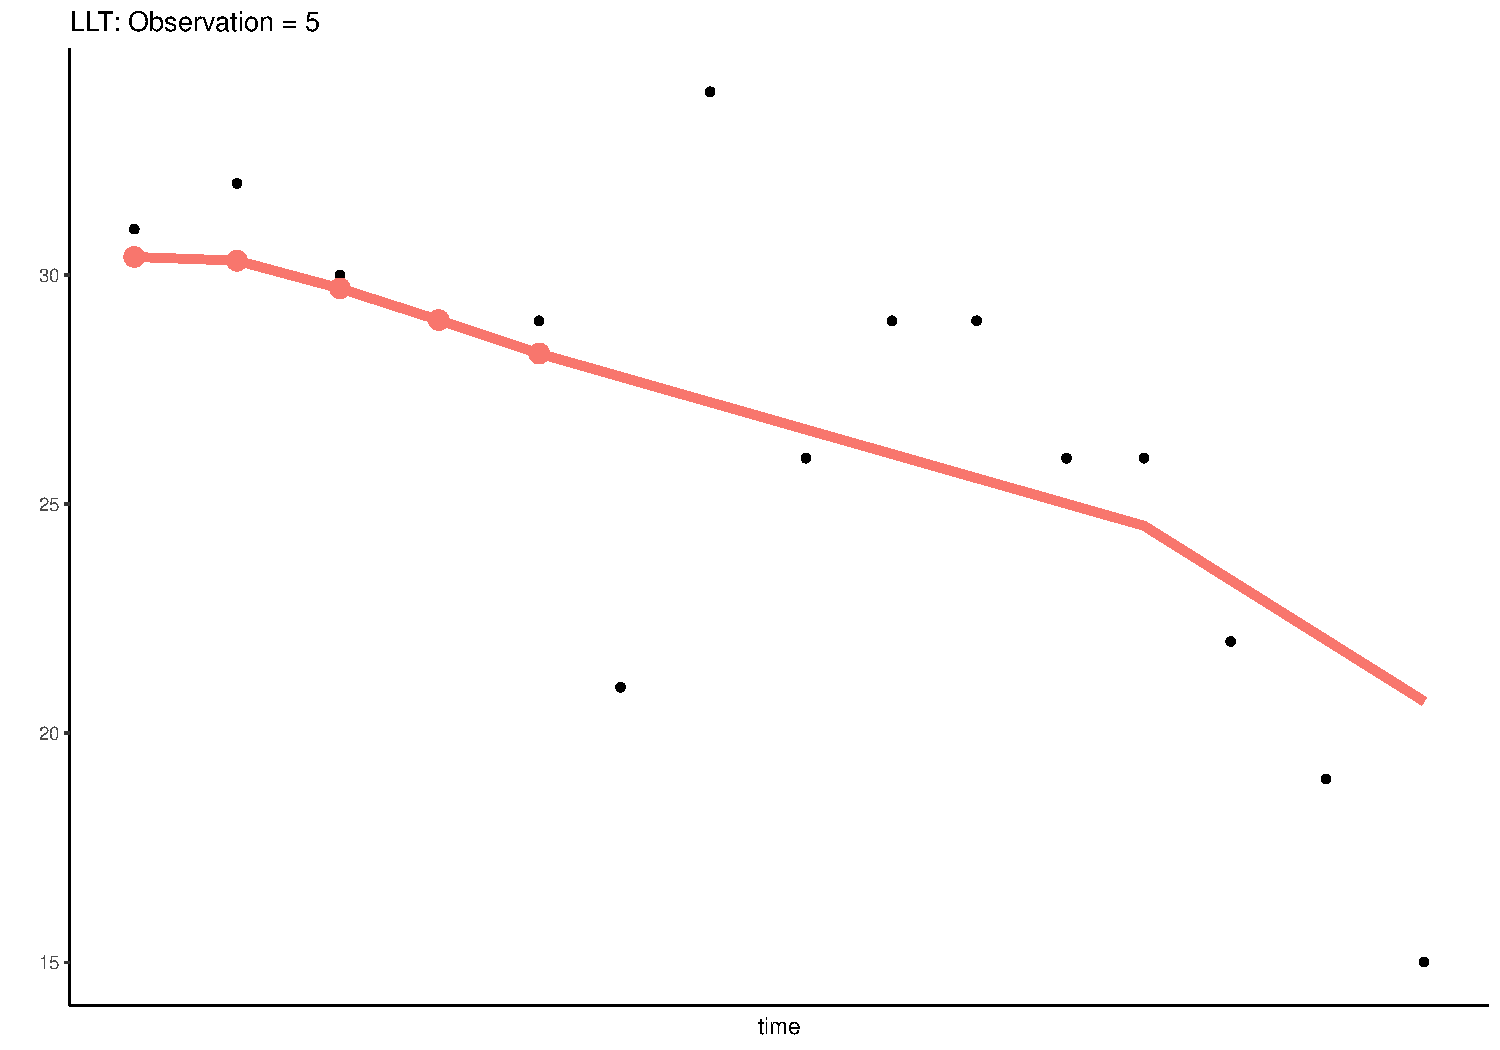
\includegraphics{Prez4_files/figure-beamer/unnamed-chunk-15-5.pdf}
\end{frame}

\begin{frame}{}
\protect\hypertarget{section-35}{}
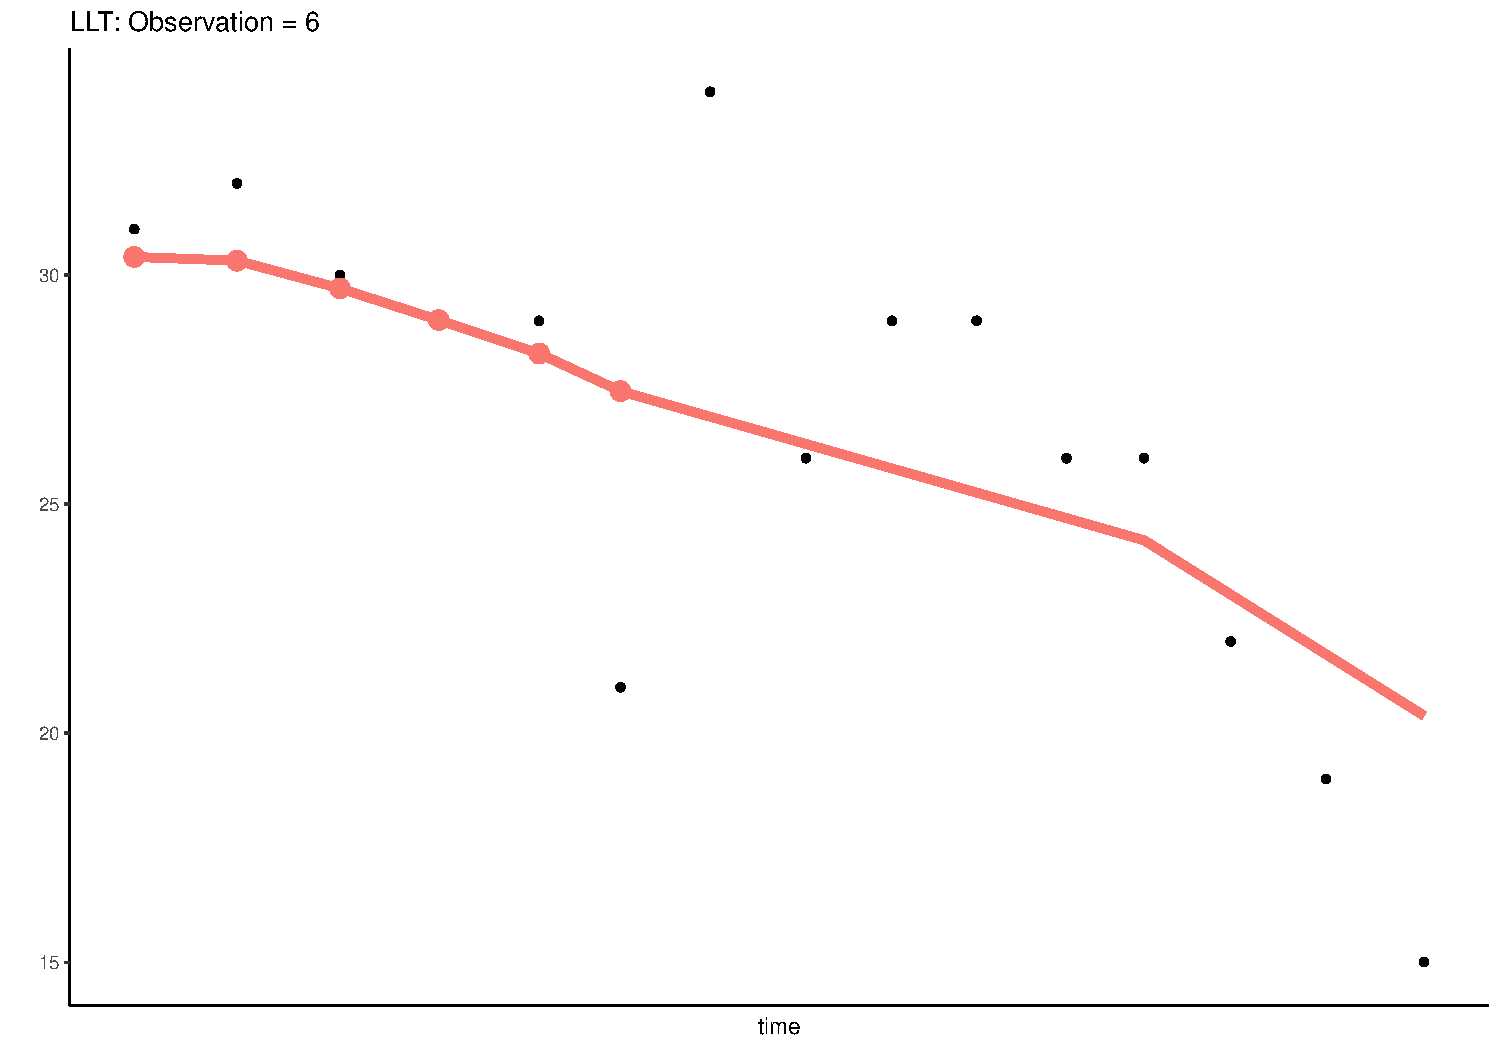
\includegraphics{Prez4_files/figure-beamer/unnamed-chunk-15-6.pdf}
\end{frame}

\begin{frame}{}
\protect\hypertarget{section-36}{}
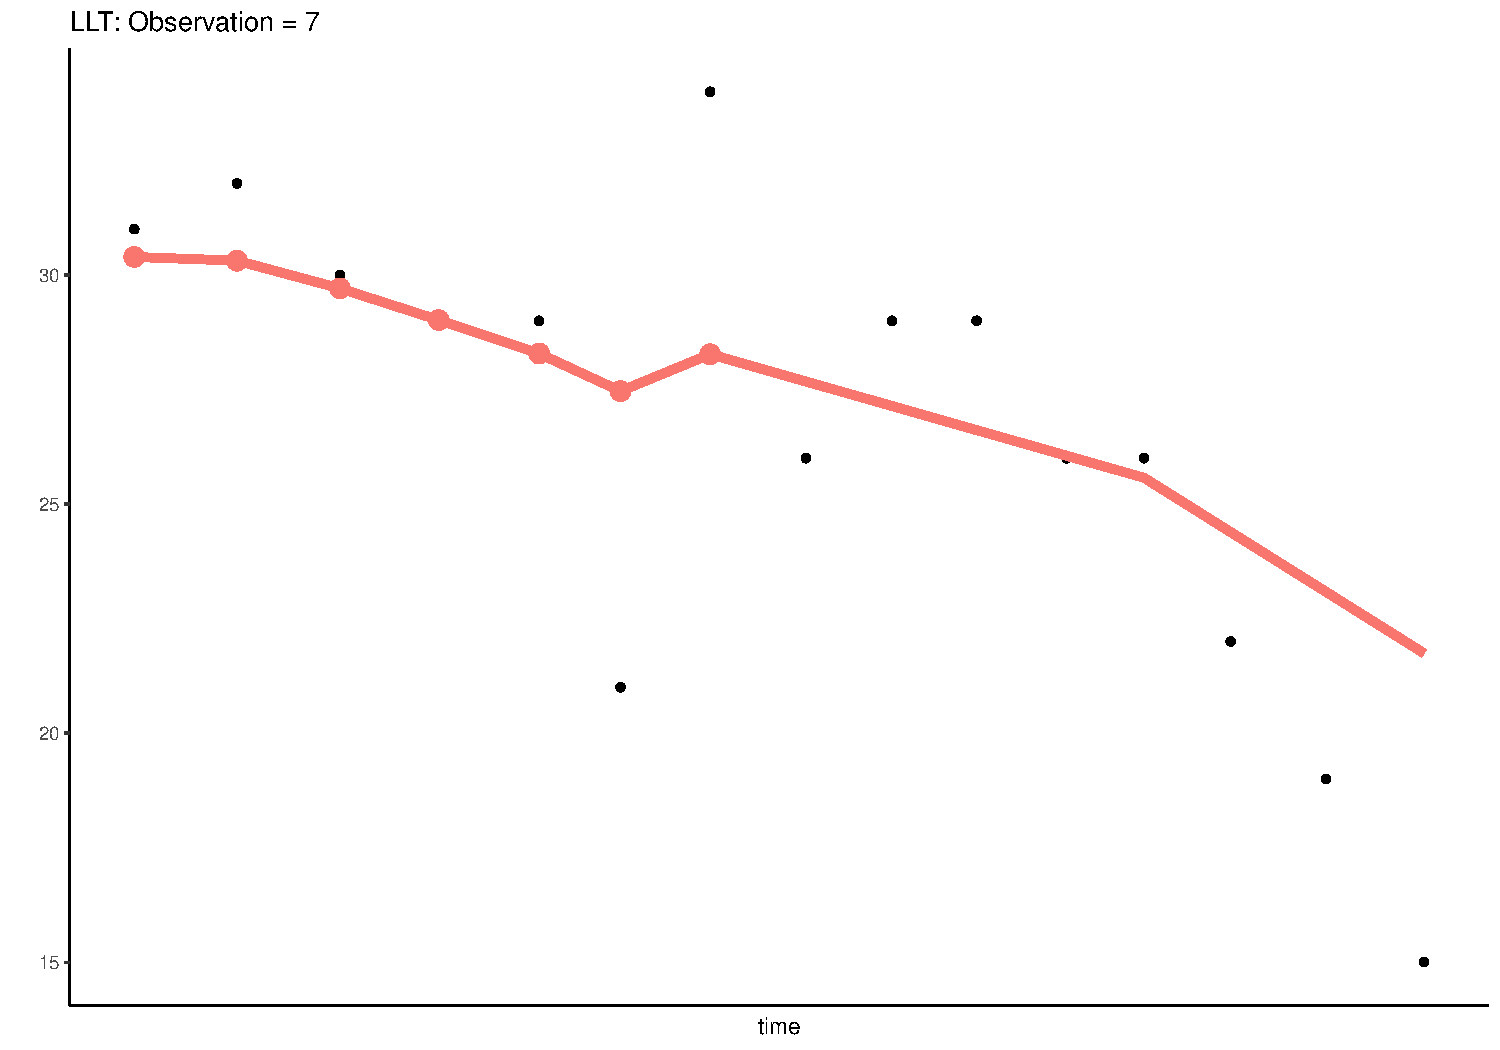
\includegraphics{Prez4_files/figure-beamer/unnamed-chunk-15-7.pdf}
\end{frame}

\begin{frame}{}
\protect\hypertarget{section-37}{}
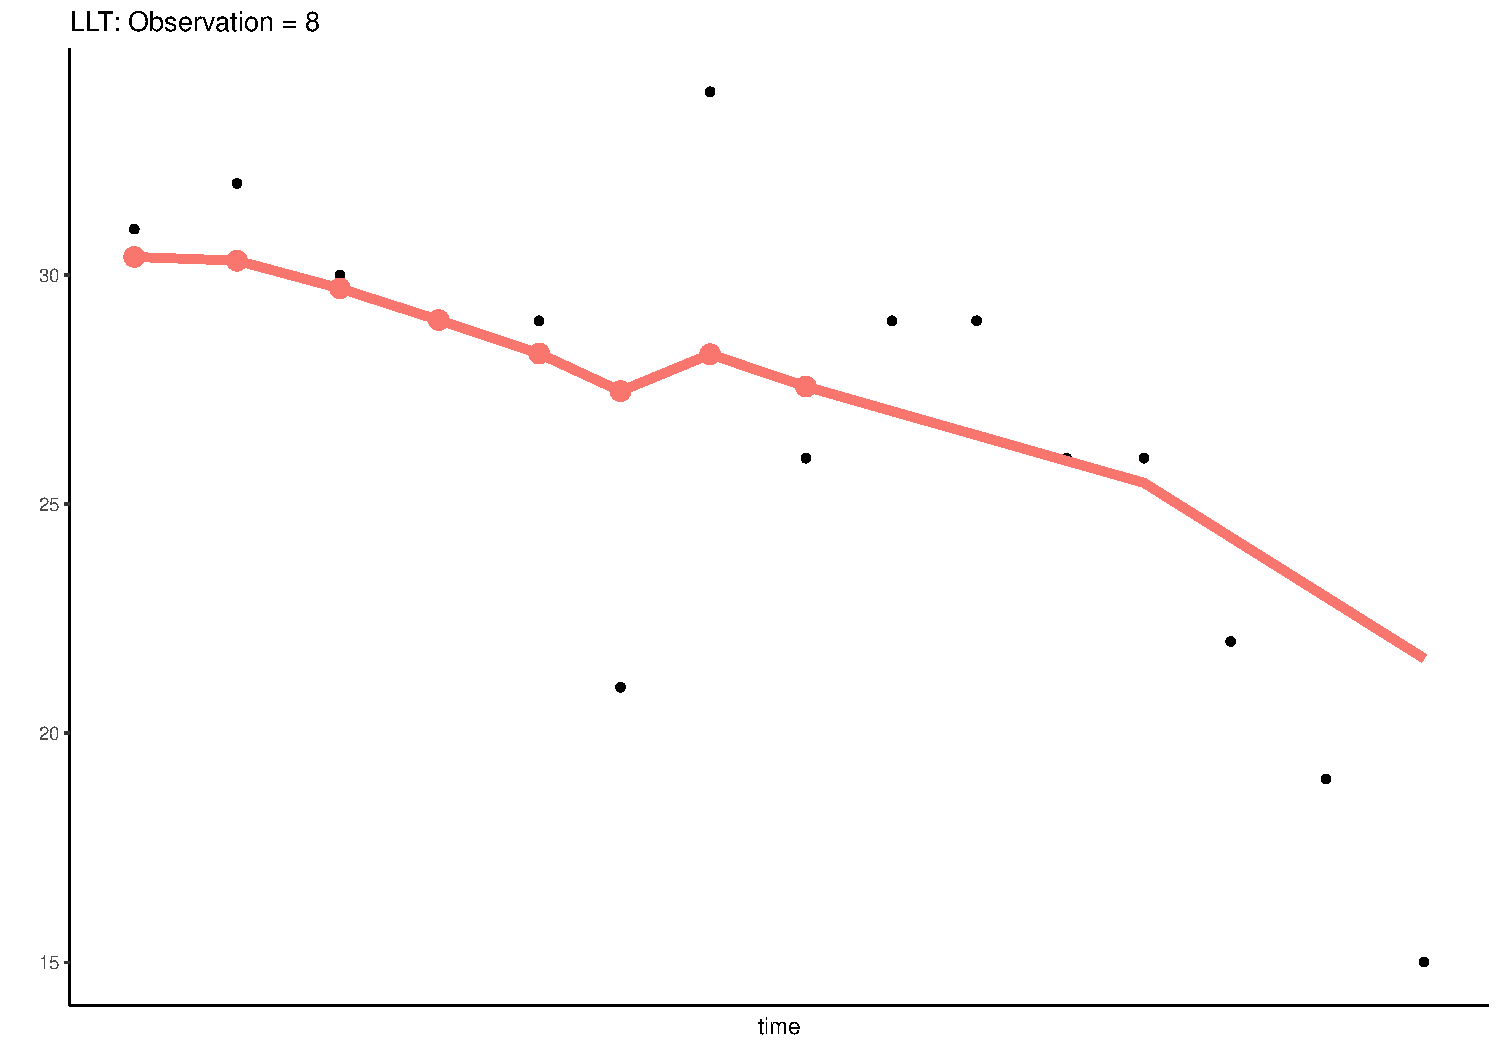
\includegraphics{Prez4_files/figure-beamer/unnamed-chunk-15-8.pdf}
\end{frame}

\begin{frame}{}
\protect\hypertarget{section-38}{}
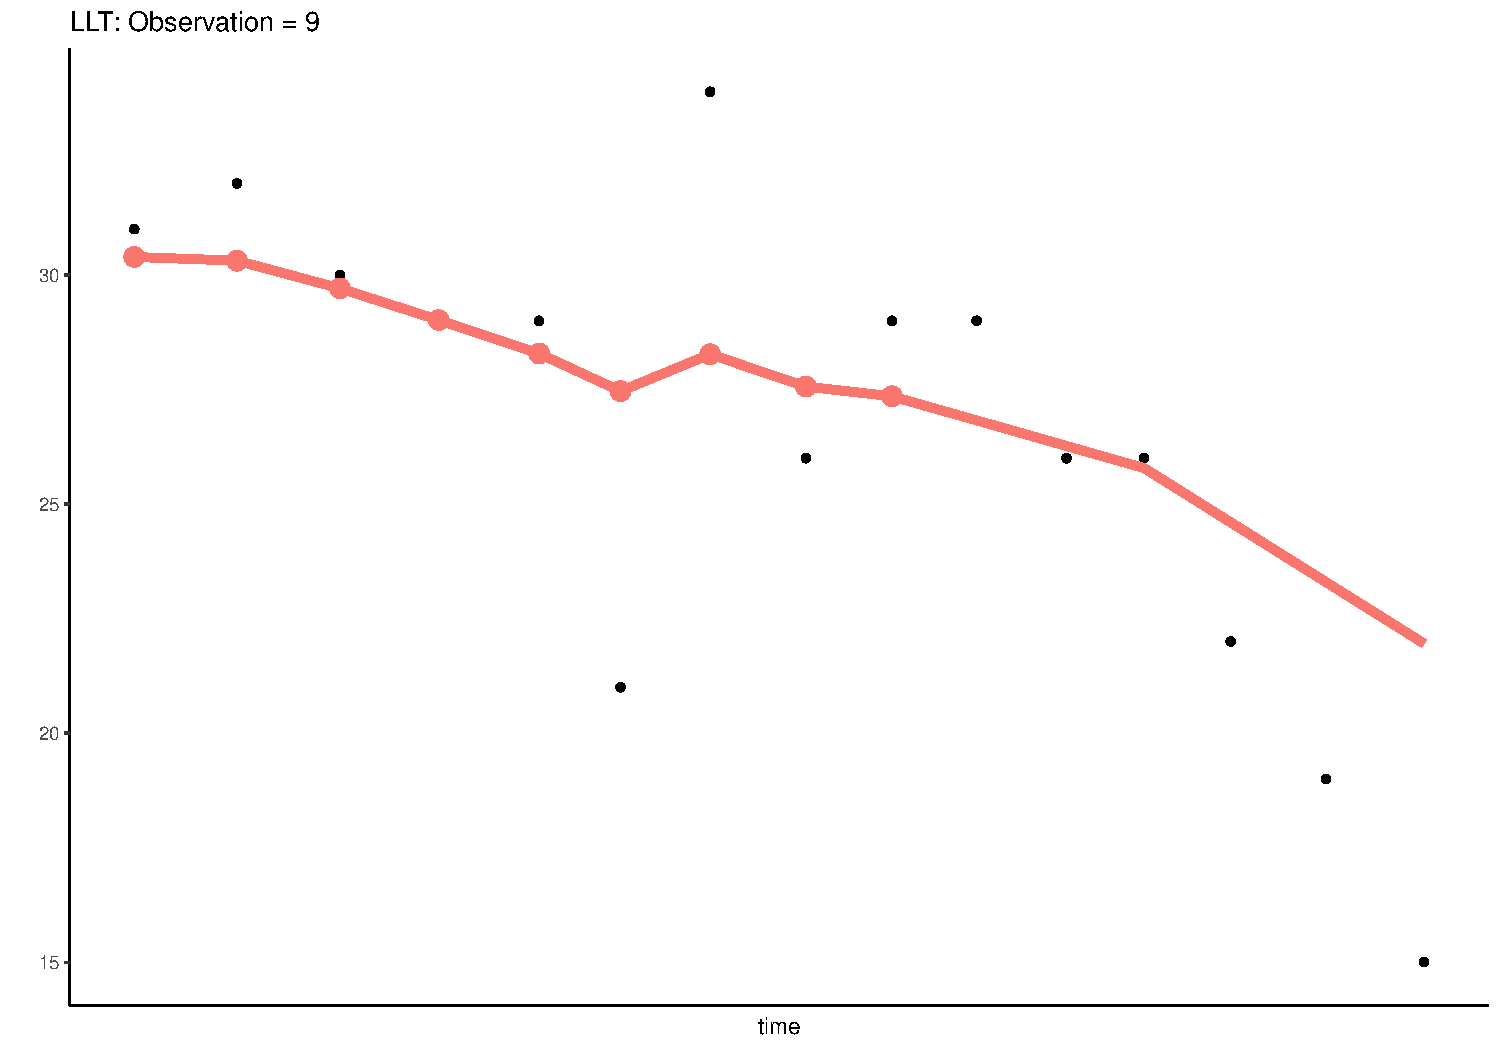
\includegraphics{Prez4_files/figure-beamer/unnamed-chunk-15-9.pdf}
\end{frame}

\begin{frame}{}
\protect\hypertarget{section-39}{}
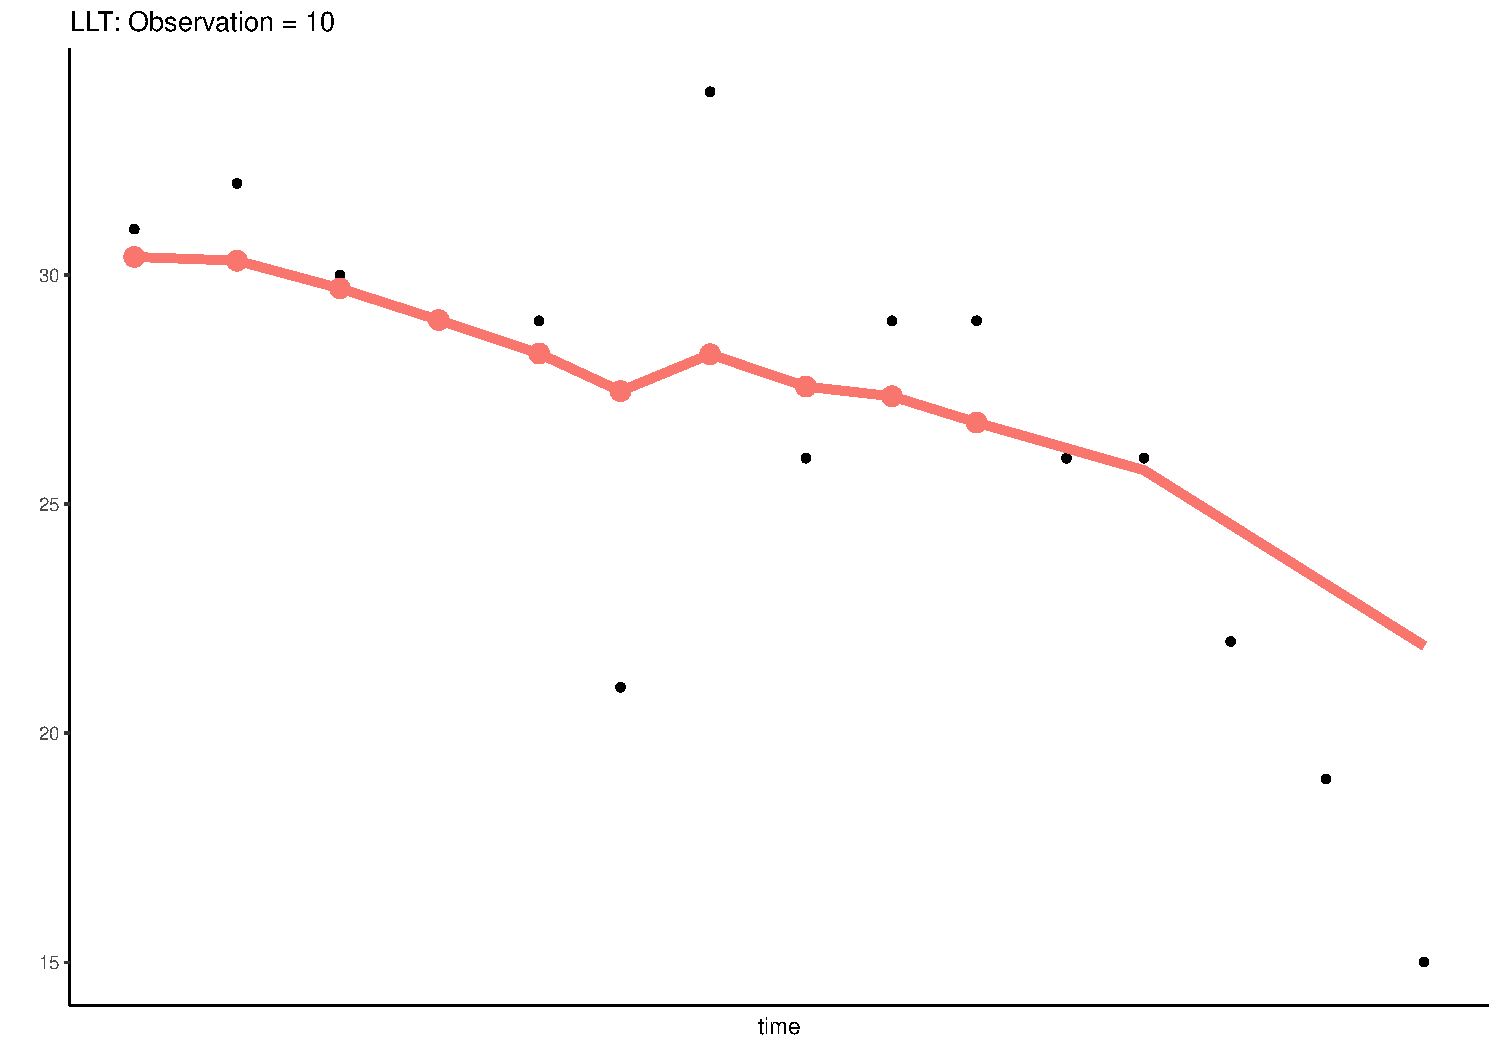
\includegraphics{Prez4_files/figure-beamer/unnamed-chunk-15-10.pdf}
\end{frame}

\begin{frame}{}
\protect\hypertarget{section-40}{}
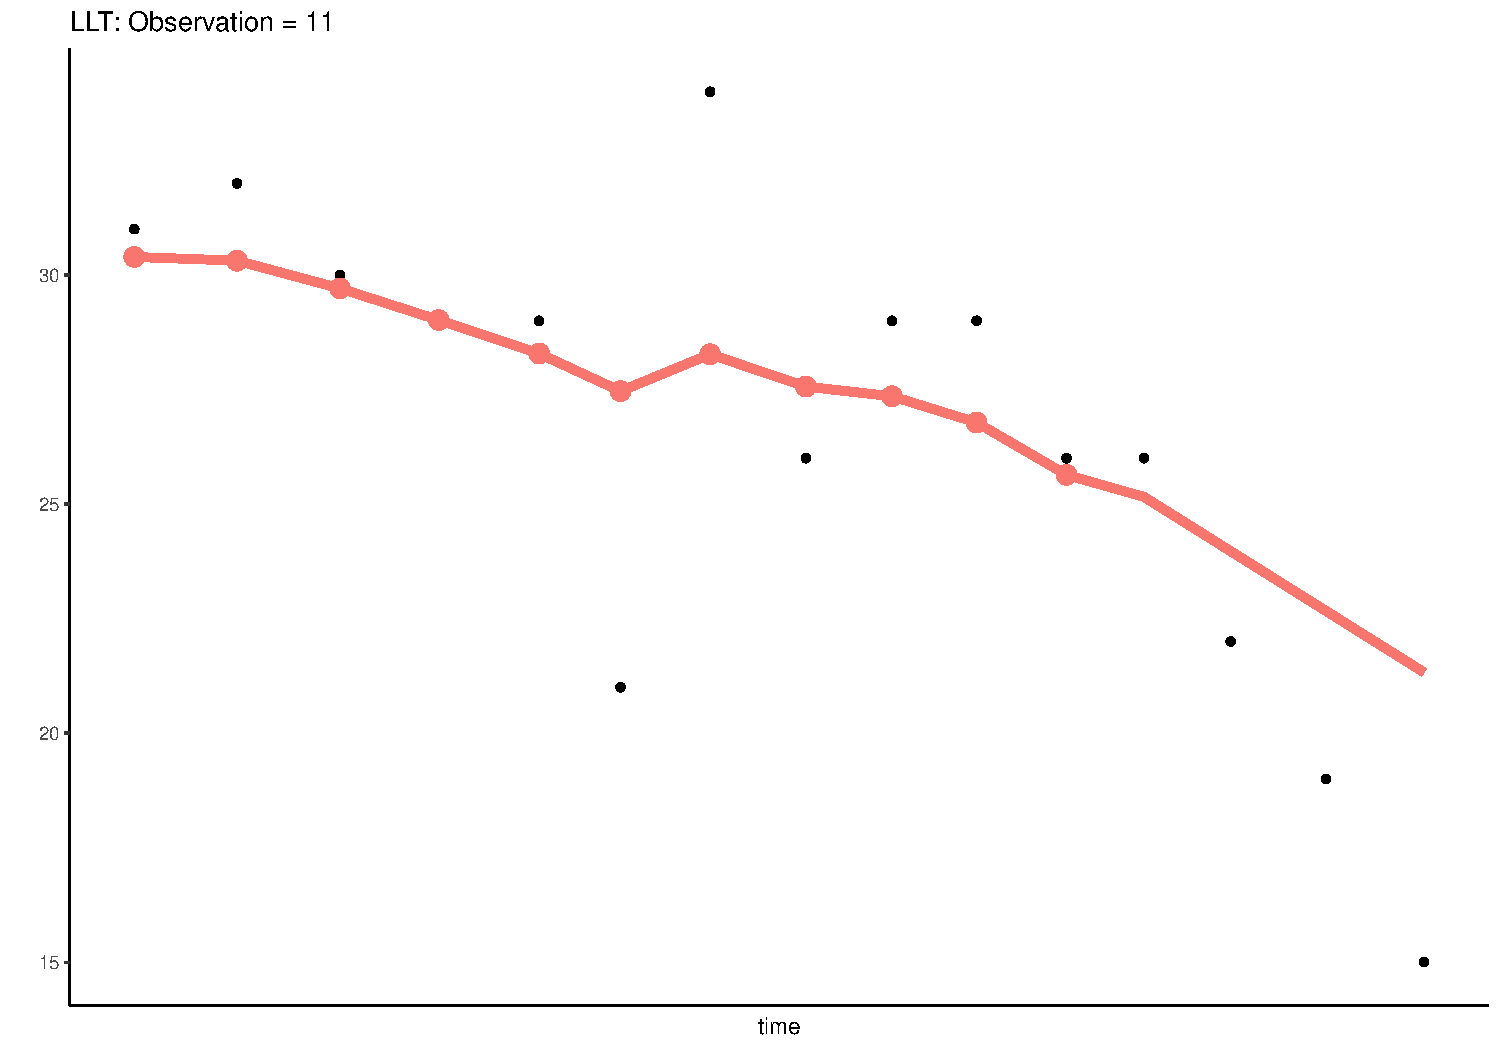
\includegraphics{Prez4_files/figure-beamer/unnamed-chunk-15-11.pdf}
\end{frame}

\begin{frame}{}
\protect\hypertarget{section-41}{}
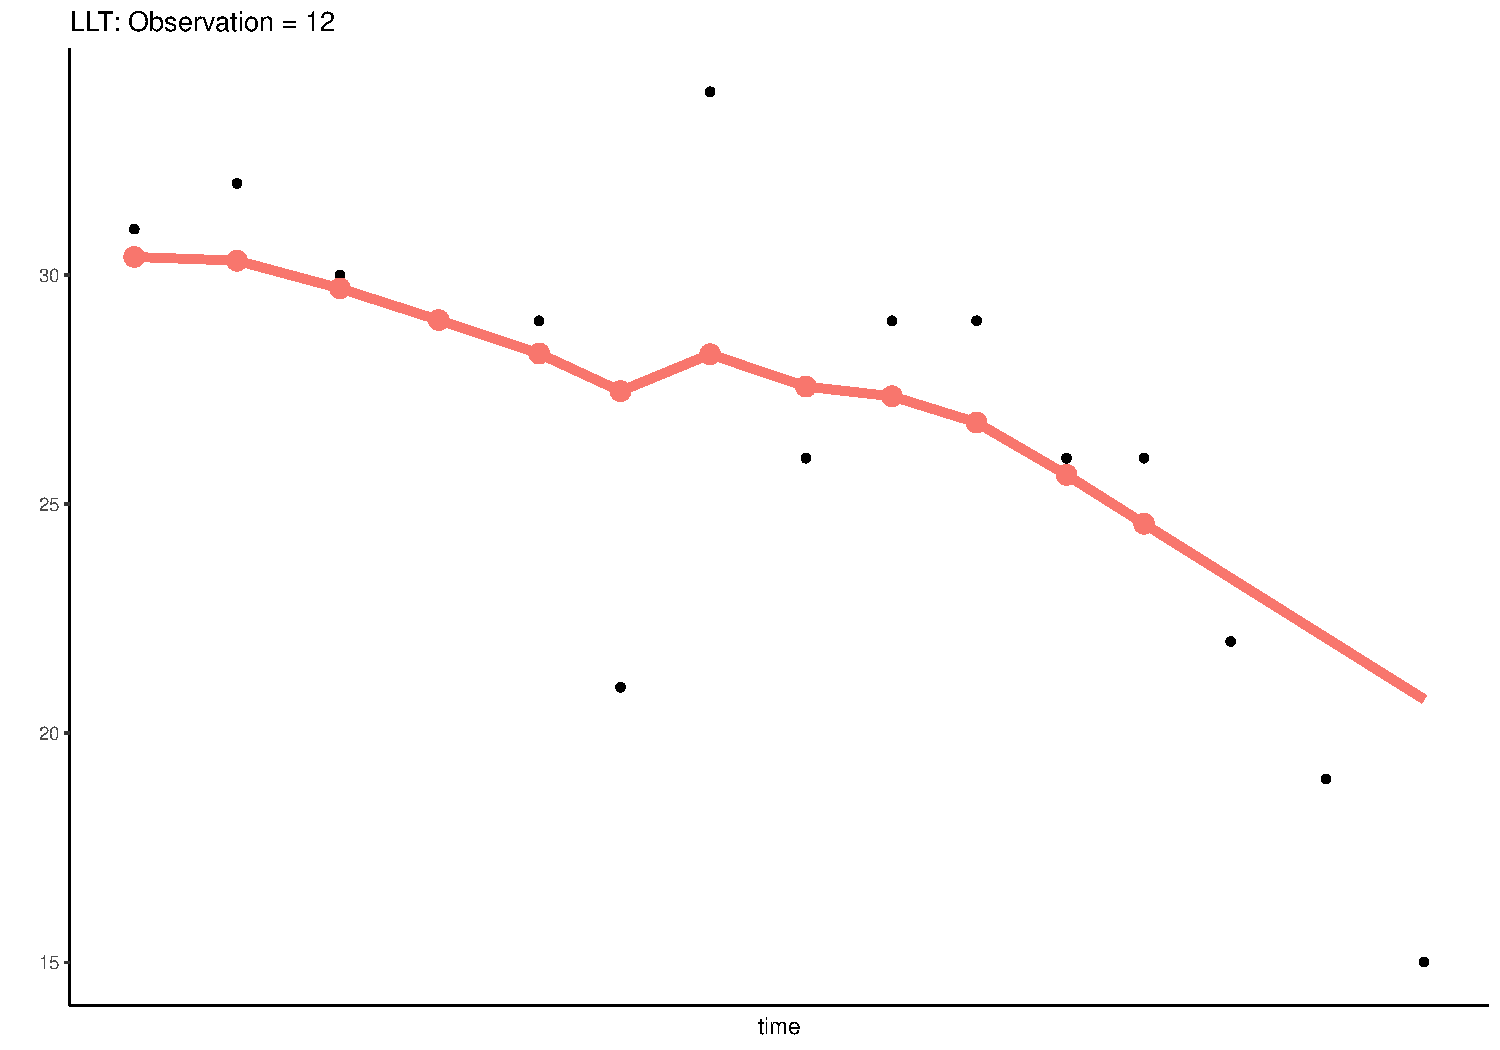
\includegraphics{Prez4_files/figure-beamer/unnamed-chunk-15-12.pdf}
\end{frame}

\begin{frame}{}
\protect\hypertarget{section-42}{}
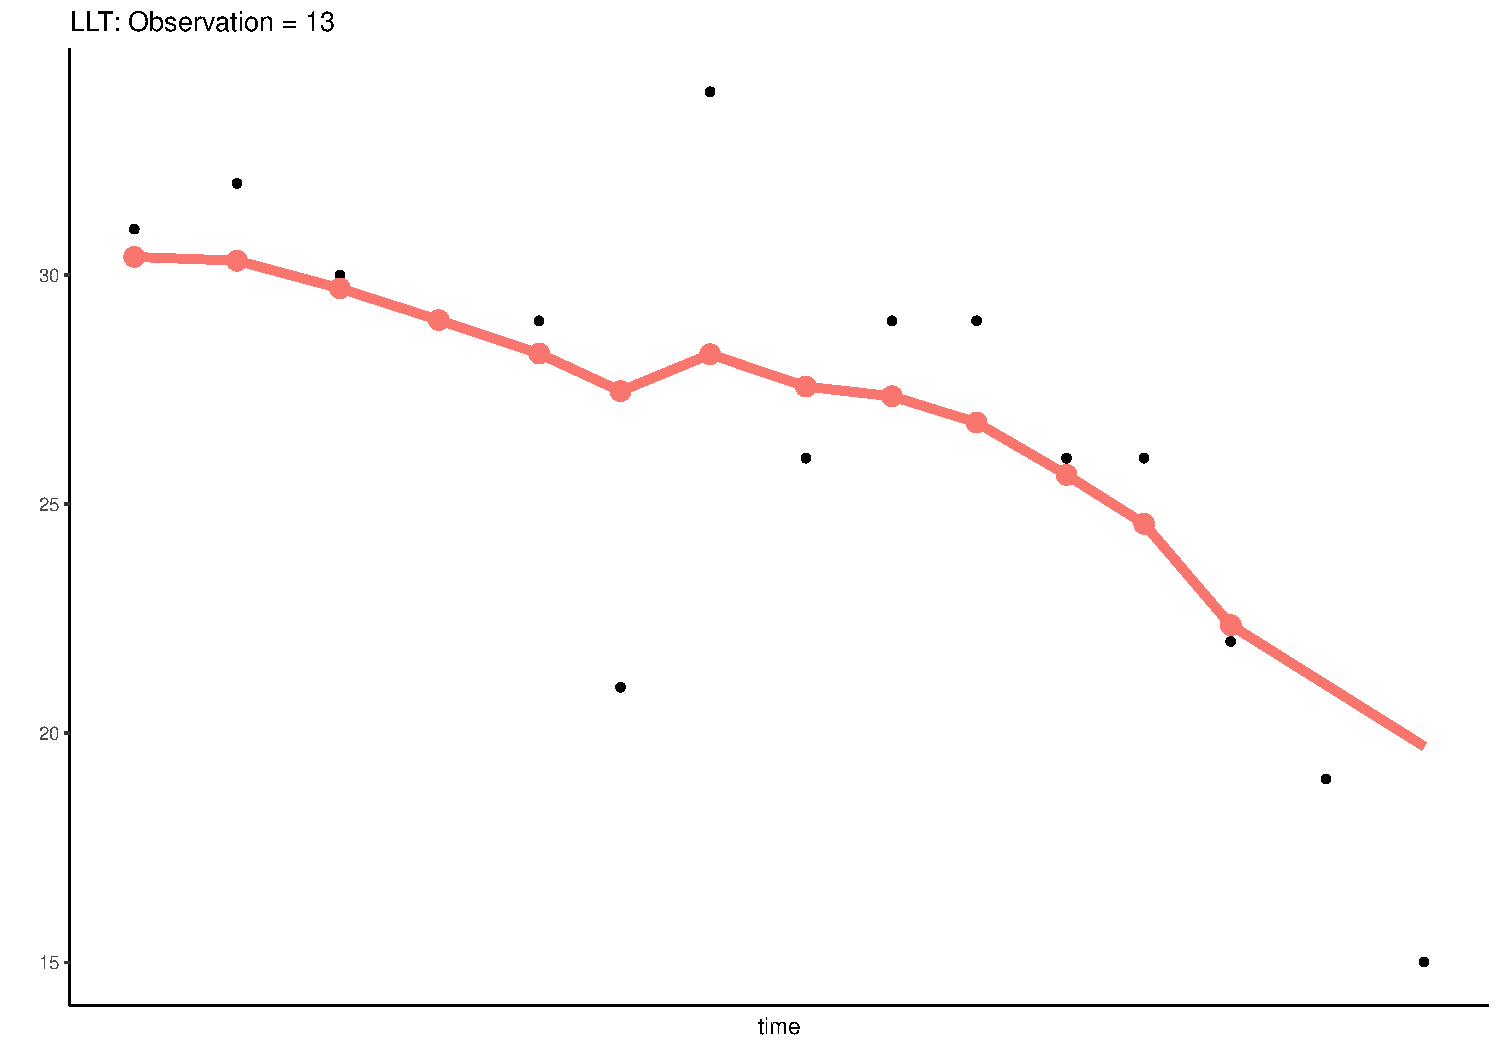
\includegraphics{Prez4_files/figure-beamer/unnamed-chunk-15-13.pdf}
\end{frame}

\begin{frame}{}
\protect\hypertarget{section-43}{}
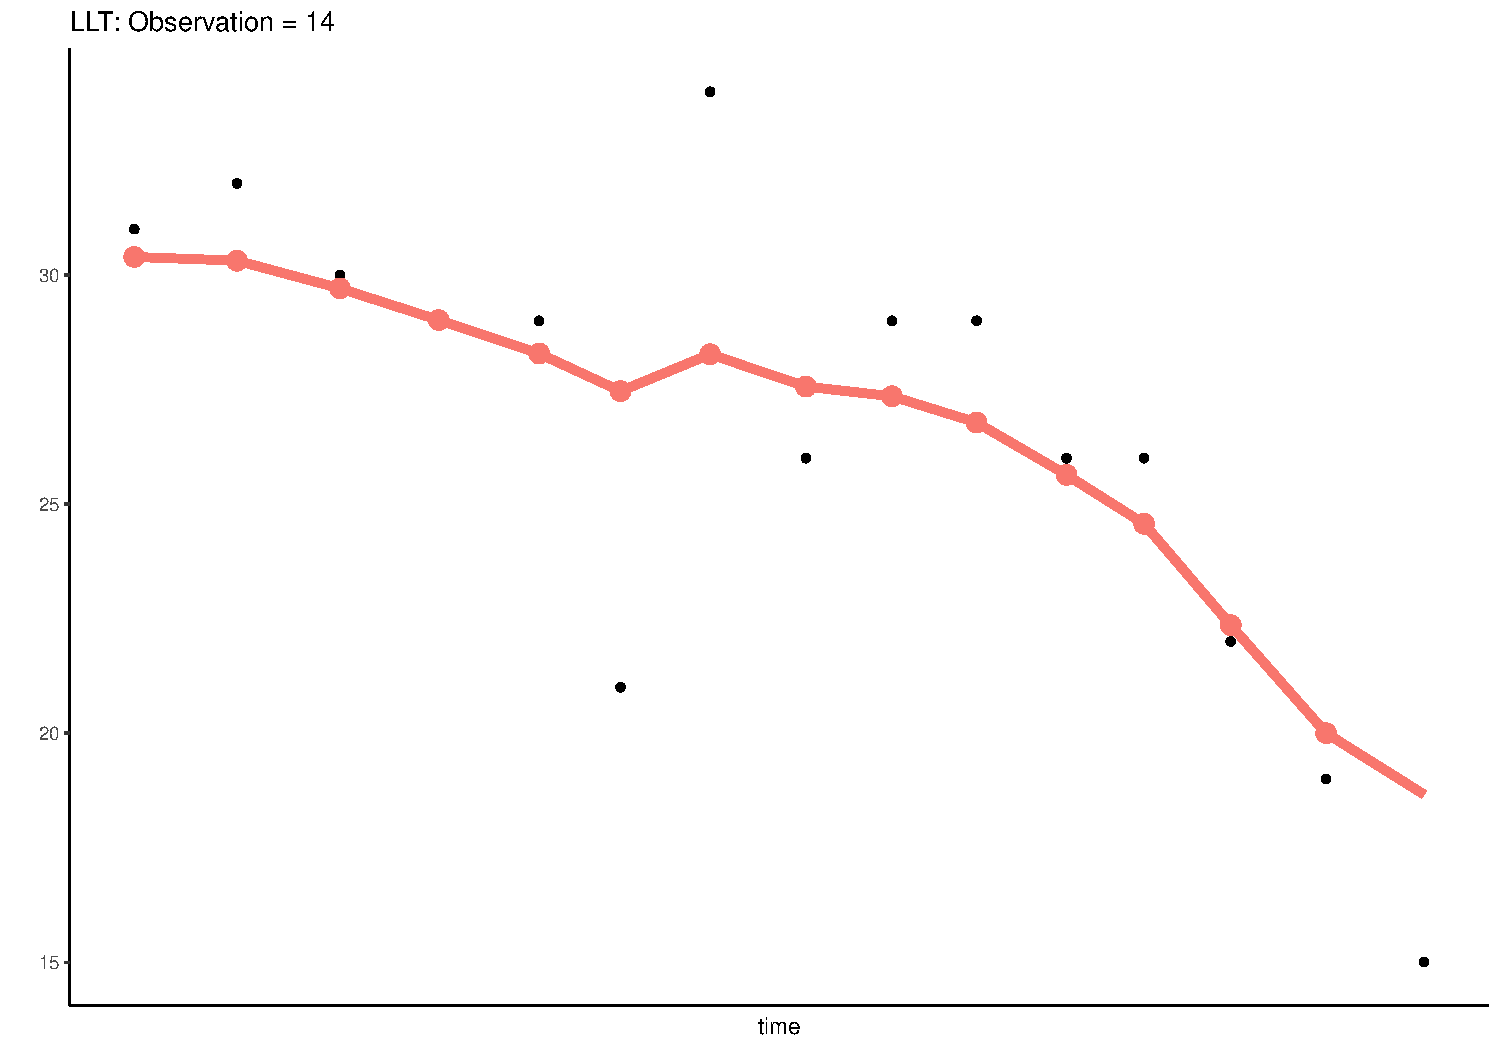
\includegraphics{Prez4_files/figure-beamer/unnamed-chunk-15-14.pdf}
\end{frame}

\begin{frame}{}
\protect\hypertarget{section-44}{}
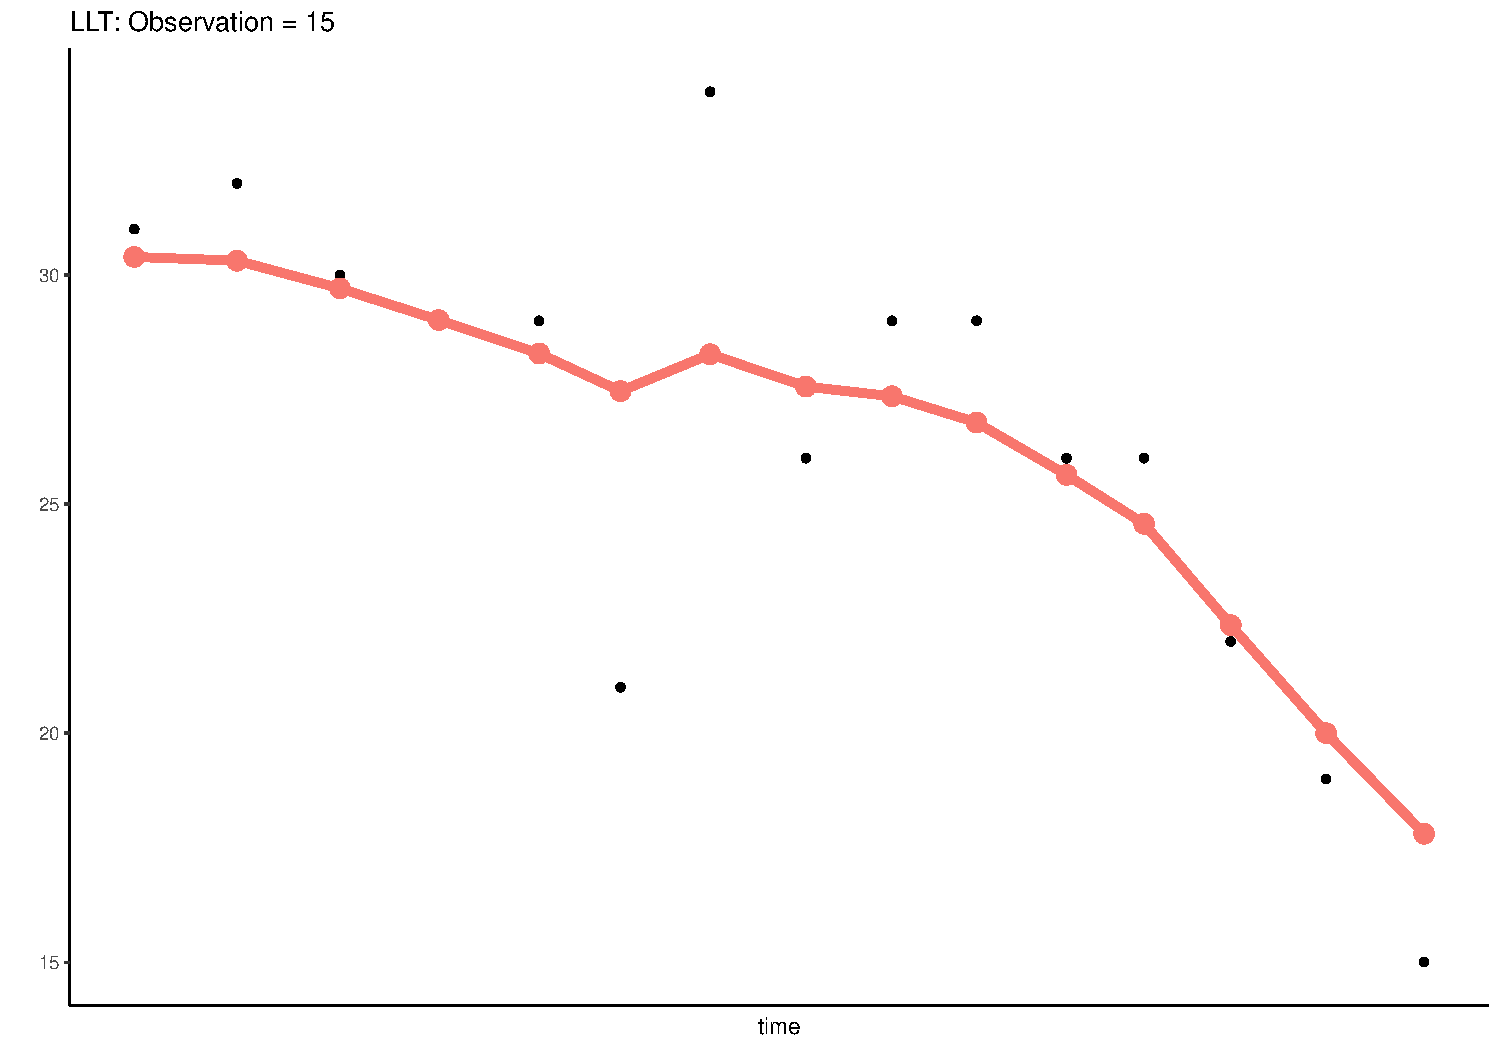
\includegraphics{Prez4_files/figure-beamer/unnamed-chunk-15-15.pdf}
\end{frame}

\begin{frame}{LLT Estimation}
\protect\hypertarget{llt-estimation}{}
We can rewrite the proposed model to fit the state space model as
follows,

\begin{align*}
y_t = 
\begin{bmatrix}
I_n & X_t
\end{bmatrix}
\begin{bmatrix}
\alpha_t\\
\beta_t
\end{bmatrix}
+ \varepsilon_t\\
\begin{bmatrix}
\alpha_t\\
\beta_t
\end{bmatrix} = 
\begin{bmatrix}
I_{(n+p) \times (n+p)}
\end{bmatrix}
\begin{bmatrix}
\alpha_{t-1}\\
\beta_{t-1}
\end{bmatrix} + 
\begin{bmatrix}
\eta_t \\
0_{p \times 1}
\end{bmatrix}
\end{align*}

\begin{columns}
\begin{column}{0.35\textwidth}
\begin{itemize}
\item $F_t = \begin{bmatrix}I_n & X_t\end{bmatrix}$
\item $v_t = \varepsilon_t$
\item $w_t = \begin{bmatrix} \eta_t \\ 0_{p\times1} \end{bmatrix}$
\end{itemize}
\end{column}
\begin{column}{0.35\textwidth}
\begin{itemize}
\item $\mu_t = \begin{bmatrix}\alpha_t \\ \beta_t\end{bmatrix}$
\item $G_t = I_{(n+p) \times (n+p)}$
\end{itemize}
\end{column}
\end{columns}
\end{frame}

\begin{frame}{Kalman Filter}
\protect\hypertarget{kalman-filter}{}
The Kalman filter is a recursive algorithm to estimate the unobserved
states conditioned on the observed data (Kalman, 1960; Durbin and
Koopman, 2012). Let \(\hat \mu_{i|j} = E(\mu_i|y_{1:j})\) and
\(P_{i|j} = var(\mu_i|y_{1:j})\).

Predicted state: \(\hat \mu_{t|t-1} = G_t \hat \mu_{t-1|t-1}\)

Predicted state covariance: \(P_{t|t-1} = G_tP_{t-1|t-1}G_t' + W\)

Innovation covariance: \(S_t = F_tP_{t|t-1}F_t' + V\)

Kalman Gain: \(K_t = P_{t|t-1}F_t'S^{-1}_t\)

Innovation: \(\tilde{f_t} = y_t - F_t \hat \mu_{t|t-1}\)

Updated state estimate:
\(\hat \mu_{t|t} = \hat \mu_{t|t-1} + K_t \tilde f_t\)

Updated state covariance: \(P_{t|t} = (I- K_tF_t)P_{t|t-1}\)

Updated innovation: \(\tilde f_{t|t} = y_t - F_t \hat \mu_{t|t}\)
\end{frame}

\begin{frame}{Kalman Smoother}
\protect\hypertarget{kalman-smoother}{}
Let \(J_t = P_{t|t} G_{t+1}' + P^{-1}_{t+1|t}\). We can then calculate
\(E(\mu_t|y_{1:T})\) and \(var(\mu_t|y_{1:T})\) using the following
Kalman smoother equations.

\begin{align*}
E(\mu_t|y_{1:T}) = \hat \mu_{t|t} + J_t (\hat \mu_{t+1|T} - \hat \mu_{t+1|t})\\
var(\mu_t|y_{1:T}) = P_{t|t} - J_t G_{t+1} P_{t|t}
\end{align*}
\end{frame}

\begin{frame}{Setting Parameters}
\protect\hypertarget{setting-parameters}{}
We assume \(\mu_0 \sim N(u_0, P_0)\), however \(u_0\) and \(P_0\) are
unknown.

\begin{itemize}
\tightlist
\item
  By initializing \(u_0 = 0\) and \(P_0 = \infty\) we are essentially
  putting a flat prior on \(\mu_0\).
\item
  It has been shown \(\hat \mu_{0|T}\) and \(P_{0|T}\) quickly converge
  to \(u_0\) and \(P_0\) respectively for even small \(T\) (Kalman,
  1960; Durbin and Koopman, 2012).
\end{itemize}

In our proposed model,
\(\mu_t = \begin{bmatrix}\alpha_t \\ \beta_t\end{bmatrix}\).

\begin{itemize}
\tightlist
\item
  \(\hat\beta_{0|T}\) is then our estimate for \(\beta\) and has
  variance covariance
  \(P_{\hat\beta} = [P_{0|T}]_{(n+1):(n+p),(n+1):(n+p)}\).
\item
  We can then use \(\hat\beta_{0|T}\) and \(P_{\hat\beta}\) for
  inference on \(\beta\).

  \begin{itemize}
  \tightlist
  \item
    \(\hat \beta \mathrel{\stackrel{\makebox[0pt]{\mbox{\normalfont\tiny asym}}}{\sim}}N(\beta, P_{\hat\beta})\).
  \end{itemize}
\end{itemize}
\end{frame}

\begin{frame}{Computational Challenges}
\protect\hypertarget{computational-challenges}{}
For each iteration of the Kalman filter we must invert
\(var(Y_t|y_{1:(t-1)}) = S_t\).

\begin{itemize}
\tightlist
\item
  \(S_t\) is non-sparse as calculating \(var(Y_t|y_{1:(t-1)})\) is a
  function of \(\beta_{t-1}\) which is shared between all observations.
\item
  \(S_t\) is an \(n \times n\), so as \(n\) increases there is an
  exponential increase in computation time.
\end{itemize}
\end{frame}

\begin{frame}{Solution 1: Partitioning}
\protect\hypertarget{solution-1-partitioning}{}
A solution to solving inversion computational inefficiencies is to
partition:

\begin{itemize}
\tightlist
\item
  Partition the subjects into \(k\) groups.
\item
  Run the Kalman filter and smoother on each group independently to
  extract \(\hat\beta_{0|T}^{(i)}\) and \(P_{\beta}^{(i)}\) for \(i\) in
  \(1, ..., k\).
\item
  Use the estimate
  \(\bar\beta = \frac{\sum_{i=1}^k\hat\beta_{0|T}^{(i)}}{k}\).

  \begin{itemize}
  \tightlist
  \item
    \(\bar \beta \sim N(\beta, \frac{\sum_{i=1}^kP_{\hat\beta^{(i)}}}{k^2})\)
  \end{itemize}
\end{itemize}
\end{frame}

\begin{frame}{Solution 2: Bayesian Gibb's Sampling Approach}
\protect\hypertarget{solution-2-bayesian-gibbs-sampling-approach}{}
\begin{itemize}
\tightlist
\item
  For the Bayesian approach we use a Gibb's sampler.
\item
  Instead of calculating \(\beta\) in the Kalman filter, we can estimate
  it separately.
\item
  The model,
\end{itemize}

\begin{equation*}
\begin{aligned}
y_t &= \alpha_t + X_t \beta +\varepsilon_t\\
\alpha_t &= \alpha_{t-1} + \eta_t
\end{aligned}
\end{equation*}
\end{frame}

\begin{frame}{Gibb's Sampling}
\protect\hypertarget{gibbs-sampling}{}
\begin{itemize}
\tightlist
\item
  Gibb's sampling is a method to gain an approximate sample from a
  posterior distribution for a given variable (Gelfand-Smith, 1990).
\item
  It works by:

  \begin{itemize}
  \tightlist
  \item
    calculating the distribution of a variable conditioned on all other
    unknown variables, known as the posterior distribution.
  \item
    sampling from the posterior distribution and assigning the new
    sample to the variable.
  \item
    calculate the posterior of the next variable and continue to sample,
    update, and recalculate the other posteriors.
  \item
    The process is commonly repeated thousands of times.
  \end{itemize}
\item
  We need to calculate the posterior for
  \(\alpha_{1:T}, \beta, \sigma^2_{\varepsilon}, \sigma^2_\eta\).
\end{itemize}
\end{frame}

\begin{frame}{Posterior of \(\alpha\)}
\protect\hypertarget{posterior-of-alpha}{}
\begin{itemize}
\tightlist
\item
  Notice, if we are conditioning on \(\beta\) for the posterior
  \(\alpha_{1:T}|...\) then each \(y_{it}\) is independent and we can
  run the Kalman filter chains independently.
\item
  Let \(y^*_t = y_t - X_t \beta\), then the model becomes
\end{itemize}

\begin{equation*}
\begin{aligned}
y^*_t &= \alpha_t +\varepsilon_t\\
\alpha_t &= \alpha_{t-1} + \eta_t
\end{aligned}
\end{equation*}

\begin{itemize}
\tightlist
\item
  We can then run a forward Kalman filter with a backward sampler to
  sample from the posterior of \(\alpha_{1:T}\) (Fruhwirth-Schnatter,
  1994)
\end{itemize}
\end{frame}

\begin{frame}{Posterior of \(\beta\)}
\protect\hypertarget{posterior-of-beta}{}
\begin{itemize}
\tightlist
\item
  We let \(\beta \sim N(\theta, \sigma^2_\beta)\)
\item
  The posterior is
  \(\beta|... \sim N(\Sigma^{-1}B, \sigma^2_\varepsilon\sigma^2_\beta\Sigma^{-1})\)
  where,
\item
  \(B = \sigma^2_\beta\big(\sum^T_{t=1}y_t-\alpha_t\big)'X_t -\sigma^2_\varepsilon\theta\)
\item
  \(\Sigma = \big(\sigma^2_\beta\sum^T_{t=1}X_t'X_t\big)+\sigma^2_\varepsilon I_p\)
\end{itemize}
\end{frame}

\begin{frame}{The Gibbs Sampling Algorithm}
\protect\hypertarget{the-gibbs-sampling-algorithm}{}
\begin{enumerate}
\tightlist
\item
  Select prior parameters for
  \(\theta, \sigma^2_\beta, a_0, b_0, c_0, d_0\).
\item
  Let \(\beta^{(0)} = \theta\),
  \(\sigma^{2(0)}_\eta = \frac{d_0/2}{1+c_0/2}\), and
  \(\sigma^{2(0)}_\varepsilon = \frac{b_0/2}{1+a_0/2}\).
\item
  Run a forward-filtering backward sampling procedure as described above
  conditioning on
  \(\beta^{i-1}, \sigma^{2(i-1)}_\eta, \sigma^{2(i-1)}_\varepsilon\) and
  set the samples equal to \(\alpha^{(i)}\) for the \(i^{th}\)
  iteration.
\item
  Sample \(\sigma^{2*}_\eta\) from
  \(IG(\frac{nT+a_0}{2}, \frac{\sum^T_{t=1} (\alpha^{(i)}_t-\alpha^{(i)}_{t-1})^2+b_0}{2})\)
  and set \(\sigma^{2(i)}_\eta = \sigma^{2*}_\eta\).
\item
  Sample \(\sigma^{2*}_\varepsilon\) from
  \(IG(\frac{nT+c_0}{2}, \frac{d_0 + \sum^T_{t=1}(y_t-X_t\beta^{(i-1)}-\alpha_t^{(i)})^2}{2})\)
  and set \(\sigma^{2(i)}_\varepsilon = \sigma^{2*}_\varepsilon\).
\item
  Sample \(\beta^*\) from
  \(N(\Sigma^{-1}B, \sigma^2_\varepsilon\sigma^2_\beta\Sigma^{-1})\)
  where
  \(\alpha = \alpha^{(i)}, \sigma^{2}_\eta = \sigma^{2(i)}_\eta, \sigma^{2}_\varepsilon=\sigma^{2(i)}_\varepsilon\)
  and set \(\beta^{(i)} = \beta^*\).
\item
  Repeat steps 3-6 for \(i\) in 1, 2, \ldots, M.
\end{enumerate}
\end{frame}

\begin{frame}{Inference on \(\beta\)}
\protect\hypertarget{inference-on-beta}{}
\begin{itemize}
\tightlist
\item
  After throwing out a number of initial samples from the Gibb's sampler
  we can estimate \(\beta\) by taking the mean of the posterior samples.
\item
  We create a \(95%
  \) credibility interval (as a pseudo-confidence interval) by
  calculating the \(2.5^{th}\) and \(97.5^{th}\) percentiles of the
  posterior draws.
\end{itemize}
\end{frame}

\begin{frame}{Simulation Analyses}
\protect\hypertarget{simulation-analyses}{}
\begin{itemize}
\tightlist
\item
  Conducted two separate simulation analyses.
\item
  The most desirable model is one that,

  \begin{itemize}
  \tightlist
  \item
    Maintains 95\% coverage of true parameter.
  \item
    Is unbiased.
  \item
    Has small parameter variance (small 95\% confidence intervals)
  \end{itemize}
\end{itemize}
\end{frame}

\begin{frame}{Simulation Study 1}
\protect\hypertarget{simulation-study-1}{}
We sampled from the models,

\begin{equation}
\begin{aligned}
y_t &= b_0 + X_t \beta + e_t, \ \ \ b_0\sim N(0, \sigma^2_b)\\
e_t &= \rho e_{t-1} + \eta_t, \ \ \ \eta_t \sim N(0, \sigma^2_\eta) 
\end{aligned}
\end{equation}

\begin{equation}
\begin{aligned}
y_t &= \alpha_t + X_t\beta + \varepsilon_t, & \varepsilon_t \sim N(0,\sigma_\varepsilon^2I_n)\\
\alpha_t &= \alpha_{t-1} +\eta_t, & \eta_t \sim N(0,\sigma_\eta^2I_n)
\end{aligned}
\end{equation}

We simulated 100 subjects to have between 3-10 observations. \(X\) was
simulated to mirror our initial model of interest from the NACC. The
variables \(\sigma^2_\varepsilon\), \(\sigma^2_\eta\), and \(\rho\)
varied between simulations. We compared 95\% CI coverage, bias, and
estimate variance between 1. LMEM with a random intercept, 2. LMEM with
a random intercept and AR(1) error correlation structure, the liklihood
state space model, the Bayesian state space model, then a state space
model partitioned into 2, 4, and 10 groups.
\end{frame}

\begin{frame}{95\% Coverage}
\protect\hypertarget{coverage}{}
\begingroup\fontsize{7}{9}\selectfont

\begin{longtable}[t]{l|l|r|r|r|r|r|r|r}
\hline
\multicolumn{2}{c|}{\makecell[c]{Variance\\Parameters}} & \multicolumn{2}{c|}{\makecell[c]{Traditional\\Methods}} & \multicolumn{5}{c}{State Space Methods} \\
\cline{1-2} \cline{3-4} \cline{5-9}
$\sigma^2_\varepsilon$ & $\sigma^2_\eta$ & LME & AR(1) & LLT & Part2 & Part4 & Part10 & Bayes\\
\hline
$\sigma^1 = 1$ & $\rho = 0$ & 0.954 & 0.953 & 0.947 & 0.952 & 0.963 & 0.983 & 0.964\\
\hline
$\sigma^1 = 1$ & $\rho = 0.1$ & 0.938 & 0.947 & 0.945 & 0.953 & 0.963 & 0.981 & 0.955\\
\hline
$\sigma^1 = 1$ & $\rho = 0.5$ & 0.889 & 0.944 & 0.965 & 0.967 & 0.977 & 0.987 & 0.962\\
\hline
$\sigma^2_\varepsilon = 3$ & $\sigma^2_\eta =0$ & 0.941 & 0.940 & 0.944 & 0.965 & 0.969 & 0.978 & 0.958\\
\hline
$\sigma^2_\varepsilon = 3$ & $\sigma^2_\eta =1$ & 0.790 & 0.847 & 0.947 & 0.948 & 0.956 & 0.972 & 0.940\\
\hline
$\sigma^2_\varepsilon = 3$ & $\sigma^2_\eta =2$ & 0.736 & 0.836 & 0.948 & 0.944 & 0.950 & 0.970 & 0.932\\
\hline
$\sigma^2_\varepsilon = 3$ & $\sigma^2_\eta =3$ & 0.715 & 0.838 & 0.946 & 0.940 & 0.945 & 0.969 & 0.928\\
\hline
$\sigma^2_\varepsilon = 30$ & $\sigma^2_\eta =10$ & 0.781 & 0.840 & 0.947 & 0.941 & 0.945 & 0.970 & 0.946\\
\hline
$\sigma^2_\varepsilon = 60$ & $\sigma^2_\eta =20$ & 0.780 & 0.840 & 0.946 & 0.944 & 0.945 & 0.967 & 0.943\\
\hline
\end{longtable}
\endgroup{}
\end{frame}

\begin{frame}{Bias and CI length}
\protect\hypertarget{bias-and-ci-length}{}
\begin{figure}
\centering
\includegraphics{Prez4_files/figure-beamer/unnamed-chunk-21-1.pdf}
\caption{Bias and confidence interval length}
\end{figure}
\end{frame}

\begin{frame}{Real Data Simulation}
\protect\hypertarget{real-data-simulation}{}
\begin{itemize}
\tightlist
\item
  Add a linear effect on the Animals outcome for half the subjects.
\item
  Estimate the model:
\end{itemize}

\begin{equation*}
\begin{aligned}
\textbf{Updated Animals} \sim & (1 + \text{I\{Transitioned to MCI or Dementia\}} + \text{APOE}\\
& + \text{Sex} + \text{APOE*Sex} + \text{Race} + \text{Age} + \text{Education}\\ 
& + \textbf{Randomized Group}) * \text{Time}
\end{aligned}
\end{equation*}

\begin{itemize}
\tightlist
\item
  Estimate the linear effect using the different models,
\item
  LMEM, LMEM AR(1), Partitioned LLT with group size 100, and Bayesian
  LLT.
\end{itemize}
\end{frame}

\begin{frame}{Bias}
\protect\hypertarget{bias}{}
\begin{figure}
\centering
\includegraphics{Prez4_files/figure-beamer/unnamed-chunk-24-1.pdf}
\caption{Parameter bias}
\end{figure}
\end{frame}

\begin{frame}{Coverage}
\protect\hypertarget{coverage-1}{}
\begin{longtable}[t]{r|r|r|r}
\hline
LMEM & LMEM AR(1) & Partition LLT & Bayesian LLT\\
\hline
0.795 & 0.889 & 0.935 & 0.94\\
\hline
\end{longtable}

\begin{itemize}
\tightlist
\item
  When the underlying data generation process is unknown, the LLT models
  do a much better estimating the effect of interest.
\end{itemize}
\end{frame}

\begin{frame}{Computation Time}
\protect\hypertarget{computation-time}{}
\begin{figure}
\centering
\includegraphics{Prez4_files/figure-beamer/compTime-1.pdf}
\caption{Computation time comparison}
\end{figure}
\end{frame}

\begin{frame}{Analysis}
\protect\hypertarget{analysis}{}
On the NACC data set we fit the model:

\begin{equation*}
\begin{aligned}
\text{Animals} \sim & (1 + \text{I\{Transitioned to MCI or Dementia\}} + \text{APOE} + \text{Sex}\\
& + \text{APOE*Sex} + \text{Race} + \text{Age} + \text{Education}) * \text{Time}
\end{aligned}
\end{equation*}

Using the LMEM, LMEM AR(1), and the Bayesian LLT Model.
\end{frame}

\begin{frame}{Results}
\protect\hypertarget{results}{}
\begin{longtable}[t]{l|l|l}
\hline
  & APOE & APOE x Sex\\
\hline
LMEM & -0.143 (-0.229, -0.058) & -0.023 (-0.128, 0.082)\\
\hline
LMEM AR(1) & -0.135 (-0.244, -0.025) & -0.049 (-0.182, 0.085)\\
\hline
Partition LLT & -0.18 (-0.36, 0) & -0.047 (-0.261, 0.167)\\
\hline
Bayesian LLT & -0.136 (-0.269, 0.011) & -0.054 (-0.23, 0.122)\\
\hline
\end{longtable}
\end{frame}

\begin{frame}{Summary}
\protect\hypertarget{summary}{}
\begin{itemize}
\tightlist
\item
  The LLT shows proper 95\% coverage for the fully simulated, even under
  model misspecification, and for the real NACC data.
\item
  When compared to the full data LLT, the partitioned LLT shows very
  similar results as long as the number of parameters estimated is
  reasonable for the group size.
\item
  The Bayesian LLT is the most desirable of the fitted models as it
  maintains 95\% coverage, is unbiased, and has the smallest parameter
  variance.
\end{itemize}
\end{frame}

\begin{frame}{Future Projects}
\protect\hypertarget{future-projects}{}
\begin{itemize}
\tightlist
\item
  Joint modeling of longitudinal outcomes using SSM framework.
\item
  Cluster analysis of longitudinal outcomes using SSM framework.
\end{itemize}
\end{frame}

\begin{frame}{Joint Modeling}
\protect\hypertarget{joint-modeling}{}
\begin{align*}
\begin{bmatrix}
y_{1ti} \\
y_{2ti} \\
y_{3ti}
\end{bmatrix} &=
\begin{bmatrix}
\mu_{1ti} \\
\mu_{2ti} \\
\mu_{3ti}
\end{bmatrix} +
x_{ti} \beta
\begin{bmatrix}
1 \\
\gamma_2 \\
\gamma_3
\end{bmatrix} +
\begin{bmatrix}
\varepsilon_{1ti} \\
\varepsilon_{2ti} \\
\varepsilon_{3ti}
\end{bmatrix} , \ \ \ \varepsilon \sim N(0, \sigma^2_\varepsilon)\\
\begin{bmatrix}
\mu_{1ti} \\
\mu_{2ti} \\
\mu_{3ti}
\end{bmatrix} &= 
\begin{bmatrix}
\mu_{1(t-1)i} \\
\mu_{2(t-1)i} \\
\mu_{3(t-1)i}
\end{bmatrix} + 
\begin{bmatrix}
\eta_{1ti} \\
\eta_{2ti} \\
\eta_{3ti}
\end{bmatrix}, \ \ \ \eta_{.ti} \sim N(0,
\begin{bmatrix}
\sigma_{\eta11} & \sigma_{\eta12} &  \sigma_{\eta13}\\
\sigma_{\eta12} & \sigma_{\eta22} &  \sigma_{\eta23}   \\
\sigma_{\eta13} & \sigma_{\eta23} &  \sigma_{\eta33}
\end{bmatrix}
)
\end{align*}
\end{frame}

\begin{frame}{Cluster Analysis}
\protect\hypertarget{cluster-analysis}{}
\begin{align*}
\begin{bmatrix}
y_{1ti} \\
y_{2ti} \\
y_{3ti} \\
y_{4ti}
\end{bmatrix} &=
\begin{bmatrix}
\mu_{1ti} \\
\mu_{1ti} \\
\mu_{2ti} \\
\mu_{2ti}
\end{bmatrix} +
x_{it} \beta
\begin{bmatrix}
1 \\
\gamma_2 \\
\gamma_3 \\
\gamma_4
\end{bmatrix} +
\begin{bmatrix}
\varepsilon_{1ti} \\
\varepsilon_{2ti} \\
\varepsilon_{3ti} \\
\varepsilon_{4ti}
\end{bmatrix} , \ \ \ \varepsilon \sim N(0, \sigma^2_\varepsilon)\\
\begin{bmatrix}
\mu_{1ti} \\
\mu_{2ti}
\end{bmatrix} &= 
\begin{bmatrix}
\mu_{1(t-1)i} \\
\mu_{2(t-1)i}
\end{bmatrix} + 
\begin{bmatrix}
\eta_{1ti} \\
\eta_{2ti}
\end{bmatrix}, \ \ \ \eta_{.ti} \sim N(0,
\begin{bmatrix}
\sigma_{\eta11} & \sigma_{\eta12}\\
\sigma_{\eta12} & \sigma_{\eta22}
\end{bmatrix}
)
\end{align*}
\end{frame}

\begin{frame}{Projected Timeline}
\protect\hypertarget{projected-timeline}{}
\begin{itemize}
\tightlist
\item
  Project 1 is under co-author review for submission.
\item
  Project 2 to be completed during fall 2021.
\item
  Project 3 to be completed during spring 2022.
\item
  Defense in the summer of 2022.
\end{itemize}
\end{frame}

\begin{frame}{Thank you!}
\protect\hypertarget{thank-you}{}
\begin{itemize}
\tightlist
\item
  Recommendations?
\item
  Questions?
\end{itemize}
\end{frame}

\end{document}
